\documentclass[a4paper,12pt,oneside]{article}

\usepackage[utf8]{inputenc}
\usepackage[T1,T2A]{fontenc}
\usepackage[english,russian]{babel}
\usepackage[usenames]{xcolor}
\usepackage{listings}
\usepackage{graphicx}
\usepackage{cmap}
\usepackage{indentfirst}
\usepackage{makeidx}

\renewcommand{\rmdefault}{cmr} 

\renewcommand{\texttt}[2][black]{\textcolor{#1}{\ttfamily #2}}

\definecolor{OliveGreen}{cmyk}{0.64,0,0.95,0.40}
\definecolor{mauve}{rgb}{0.58,0,0.82}

\setlength{\parskip}{6pt}

\makeindex

\title{Лекции по C++}
\author{Владимиров Константин Игоревич}
\date{2013-04-02}

\begin{document}

\begin{titlepage}
\begin{center}

\large ~ \\[4.5cm]

\huge Курс лекций\\[0.6cm]
\large По языку программирования C++\\[3.7cm]

\begin{minipage}{0.5\textwidth} % начало маленькой врезки в половину ширины текста
\begin{flushleft} % выровнять её содержимое по левому краю
\emph{Автор:} Владимиров К. И.\\
\end{flushleft} % конец выравнивания по левому краю
\end{minipage} % конец врезки

\vfill

{\large \today}
{\large \LaTeX}

\end{center}
\thispagestyle{empty}
\end{titlepage}

\tableofcontents

\lstset{
language=C++,                           % Code langugage
basicstyle=\ttfamily,                   % Code font, Examples: \footnotesize, \ttfamily
keywordstyle=\color{OliveGreen},        % Keywords font ('*' = uppercase)
commentstyle=\color{gray},              % Comments font
stringstyle=\color{mauve},
numbers=left,                           % Line nums position
numberstyle=\tiny,
numbersep=10pt,
stepnumber=1,                           % Step between two line-numbers
frame=none,                             % A frame around the code
tabsize=2,                              % Default tab size
captionpos=b,                           % Caption-position = bottom
breaklines=true,                        % Automatic line breaking?
breakatwhitespace=false,                % Automatic breaks only at whitespace?
showspaces=false,                       % Dont make spaces visible
showstringspaces=false,
showtabs=false,                         % Dont make tabls visible
columns=flexible,                       % Column format
title=\lstname,
caption={},
extendedchars=\true,
inputencoding=utf8,
}

\pagebreak
\section{Общие сведения}

С++ (произносится ``си плас плас'')\index{C++} это язык общего назначения с сильной статической типизацией и ручным управлением ресурсами. Де-факто в современном программировании C++ является индустриальным стандартом. Язык был создан Бьярном Строструпом\index{Stroustrup} в 1980-м году как объектно-ориентированное расширение языка C\index{C}, известного с 70-х. В 1985-м появилась первая коммерческая версия компилятора Cfront и по языку была опубликована первая книга. 

По прошествии времени, C++ был принят сообществом, широко распространился на различных архитектурах и операционных системах. В 1998-м году язык C++ был стандартизован (работа велась с 1990-го года). Сейчас язык C++ имеет развитую инфраструктуру средств компиляции, отладки, библиотек, поддержку в IDE. Много новых возможностей было введено в язык новым стандартом, принятым в 2011-м году.

\subsection{Стандартизация C++}

Вопрос к студентам: что такое ISO\index{ISO standard}, какие стандарты ISO вы знаете (читали).

Первый стандарт языка C++ под кодовым номером ISO/IEC 14882-1998 \cite{stdcpp98} был написан и утверждён ISO в 1998 году. Он включает в себя по нормативной ссылке стандарт языка C, ISO/IEC 9899-1990 \cite{stdc90}, что означает следующее: 
\begin{itemize}
\item
Возможности C90 (кроме явно оговоренных исключений) также являются возможностями C++98, также и стандартная библиотека языка C в ревизии C90 является стандартной библиотекой C++98
\item
Новые возможности C99 \cite{stdc90} не являются возможностями C++98 (стоит отметить, что стандарт C99 включён по ссылке в C++11 \cite{stdcpp11}, но стандарт C11 \cite{stdc11} снова разошёлся с текущим нижележащим подмножеством C в C++)
\end{itemize}

Стандарт языка C++ традиционно отличается от стандарта языка C тем, что стандарт C определяет корректность программы, написанной на C, стандарт же C++ определяет корректность компилятора. Это различие с первого раза кажется несущественным и бюрократическим, но во многом из-за него, например, стандарт C99 никогда не был целиком реализован ни в одном компиляторе C, поскольку конформные программы можно писать и с подмножеством возможностей. В то же время гораздо более сложный C++98 был реализован в некоторых компиляторах даже в своих наиболее эзотерических частях, таких как экспорт шаблонов.

Любой код, подаваемый на вход удовлетворяющего стандарту компилятора, стандарт классифицирует на следующие типы:
\begin{itemize}
\item
 \textbf{Syntax violation}\index{Syntax violation} -- нечто, вообще не являющееся кодом на языке C++. Это наиболее распространённый вид кода, производимого программистами.
\item
 \textbf{Implementation defined}\index{Implementation defined} – зависящий от разработчика и документации конкретного компилятора. Пример – как ведёт себя знаковое целое при сдвиге вправо.
\item
 \textbf{Unspecified}\index{Unspecified} – поведение корректного кода, не регламентированное стандартом. 
 Пример – порядок выполнения аргументов у функции.
\item
 \textbf{Undefined behavior}\index{Undefined behavior} – поведение некорректного кода, не запрещённое стандартом. 
 Пример – поведение целого числа при переполнении.
\item
 \textbf{Strictly conforming}\index{Strictly conforming} – хороший, полностью удовлетворяющий стандарту код, не выходящий за пределы стандарта. ``In anima vili'' редко встречается за пределами hello world у профессионалов и никогда не встречается у новичков.
\item
 \textbf{Conforming}\index{Conforming} – код удовлетворяющий стандарту + использующий implementation defined features.
\end{itemize}

У разных компиляторов есть своя стратегия выдачи диагностических сообщений. Для компиляции большинства примеров из этих лекций, будет использован компилятор g++ версии 4.7.1 или выше, входящий в GNU Compiler Collection с опциями: 

\lstinline!g++ -pedantic-errors -Wall -Werror -g3 -O0 -std=c++98!

\lstinline!g++ -pedantic-errors -Wall -Werror -g3 -O0 -std=c++11!

Эти опции заставляют репортить о не-conforming коде и воспринимать все диагностические сообщения как ошибки, а также включать отладочную информацию включая отладку по макросам и отключать все оптимизации (с моей точки зрения это единственный приемлимый способ компиляции учебных примеров).

Пример conforming кода на C-подмножестве C++:

\lstinputlisting{cpp_code/p0s1.cpp}

Приведённый выше код является conforming но не strictly conforming из-за использования INT\_MAX, являющегося implementation-defined. Тем не менее, нет способа заставить GCC выдать такое диагностическое предупреждение и этот код проходит компиляцию без ошибок, так что можно считать уровень conforming достаточным.

\pagebreak
\subsection{Неопределенное поведение}

Изо всех рассмотренных выше видов поведения программы, самое страшное это неопределённое поведение (undefined behavior или для краткости UB). Любой программист на языке C++ с опытом развивает чутьё на неопределённые ситуации, но даже профессионалы часто попадаются на эту удочку. В этих лекциях я предпочитаю остановиться на этой теме с самого начала, поскольку чутьё на такие ситуации надо развивать сразу. Сначала эффектный пример.

\subsubsection{Неявное UB как путь к проклятию}

Следующий код на C++ выглядит достаточно невинно

\begin{lstlisting}
#include <iostream>

int
main ()
{
  int i;

  for (i = 0; i < 10; ++i)
    std::cout << i << " : " << i*1000000000 << " : " << std::endl;

  return 0;
}
\end{lstlisting}

Но в эксперименте с GCC 4.8.2 мы получаем (в случае INT\_MAX = $2^{31} - 1$) бесконечный цикл. Компилятор на этапе agressive-loop-optimizations, считает, что без переполнения i не может быть больше 2. А раз 2 < 10, то и выход по условию (i < 10) невозможен, так что его и проверять не стоит.

Этот пример показателен тем, что в случае UB компилятор может не только \textbf{сделать} всё что угодно (например отформатировать диск), но и \textbf{не сделать} чего-то, причём компилятор даже не обязан об этом сообщать.

\subsubsection{Типичные случаи неопределённого поведения}

Здесь будет рассмотрен только язык C и C-подмножество C++. Неопределённое поведение возникающее при работе с ООП и шаблонами будет рассмотрено в конце соответствующих частей, а вот C вы уже должны знать. Типичными случаями, когда вы можете ожидать неопределённого поведения являются:

\textbf {Арифметика}
\begin {itemize}
\item Целочисленное переполнение
\item Математическая неопределенность результата (скажем деление на 0)
\item Сдвиг влево на отрицательные значения
\item Сдвиг на значения, превышающие размер типа
\item Приведение целого числа к не вмещающему его типу
\item Попытка изменить константный объект, приведя его к не константному
\end {itemize}

\textbf {Указатели}
\begin {itemize}
\item Разыменование нулевого указателя
\item Разыменование неинициализированного указателя
\item Разыменование указателя на память, динамически выделенную с нулевым размером
\item Использование указателей и ссылок на объекты с истекшим сроком жизни
\item Адресная арифметика с результатом выходящим за границы массива и доступ к такой памяти
\item Преобразование указателей в несовместимые типы
\item Использование memcpy на пересекающихся участках памяти
\end {itemize}

\textbf {Препроцессор}
\begin {itemize}
\item Непустой исходный файл, не оканчивающийся на пустую строку (или оканчивающийся на обратный слеш)
\item Обратный слеш после которого стоит нечто отличное от перечня escape-кодов
\item Выход за реализационные пределы (скажем 1024 условия в switch)
\item Динамически генерируемый токен под \lstinline!#if!
\end {itemize}

Разумеется этот список не претендует на полноту, но он даёт представление о местах, которых стоит опасаться.

\subsubsection{Пример исправления ситуации}

Очень часто код, демонстрирующий неопределённое поведение, можно переписать на эквивалентный детерминированный. Это работает не во всех случаях, но гораздо чаще, чем многие думают. Типичный грозящий UB код:

\begin{lstlisting}
int foo(int a) 
{
  assert(a + 100 > a); /* ORLY? */
  printf("%d %d\n", a + 100, a);
  return a;
}
\end{lstlisting}

Автор этого кода скорее всего считает, что оградился от случаев арифметичесого переполнения. На самом деле он просто заложился на неопределенное поведение. Простое переписывание кода сделает его гораздо более безопасным:

\begin{lstlisting}
int foo(int a) 
{
  assert(a < (INT_MAX - 100));
  printf("%d %d\n", a + 100, a);
  return a;
}
\end{lstlisting}

Если исправление ситуации с неопределённым поведением в ваших силах -- делайте это.

\subsection{Важность стандартизации}

Стандарты и даже ошибки в стандартах отлиты в граните. Например, в стандарте IEEE POSIX 1003.1-1988 была допущена ошибка: в одной главе было указано, что \lstinline!PATH_MAX! включает terminating null, в то время, как в другой главе было указано что не включает. Ошибка была обнаружена после публикации стандарта, люди обратились в комиссию стандартизации и оттуда пришло объяснение, что если написано и так и так, значит может быть и так и так. Хотя изначально идея была как раз в том, чтобы определённо установить включает ли \lstinline!PATH_MAX! нулевой символ.

Язык как соглашение между программистами и разработчиками компиляторов утверждается своим стандартом и не существует вне его. Все стандарты ISO доступны бесплатно в версии final draft – последнего черновика перед утверждением. Часто пиратски доступны и окончательные версии.

Читать и понимать стандарт языка – то, чем занимается каждый программист при решении любых спорных вопросов, возникающих у него относительно тех или иных языковых средств. Это последняя и окончательная инстанция.

Все эти лекции можно считать приглашением к самостоятельной проработке стандарта C++ совместно с решением практических задач. Собственно чтобы научится писать программы, надо знать язык и писать программы, иных вариантов нет.

\subsection{С++ это конгломерат языковых возможностей}

При изучении C++ необходимо понимать, что C++ не является монолитным языком (как C), а является сложным, исторически сформировавшимся конгломератом возможностей, зачастую порождающих взаимоисключающие стили решения конкретных задач. Кроме того, язык имеет много ``почти стандартных'' библиотек и популярные расширения на конкретных компиляторах. Самые известные это GNU расширения для C и C++, позволяющие, например, использовать в языке C вложенные функции и возвращать результат выполнения блока из фигурных скобок.
\paragraph{}
Поэтому всегда, когда вы пишете на C++, вы на самом деле пользуетесь неким его подмножеством или надмножеством, логическим или же техническим. Эти лекции охватывают (в указанном порядке) следующие основные подмножества C++:
\begin{itemize}
\item
Old plain C – подмножество C в языке C++, основные сложности, сходства и отличия
\item
Object-oriented С++ – объектно-ориентированные возможности в C++
\item
Template meta-programming – шаблоны и метапрограммирование
\item
STL – стандартную библиотеку, её основные идеи и возможности
\item
Exceptional C++ – исключения, гарантии исключений, проектирование с учётом исключений
\item
Функционал нового стандарта C++11 – rvalue references и  lambda-expressions
\item
Расширения GNU, популярные библиотеки, в частности Boost и ``несовершенные'' решения в языке
\end{itemize}

Для успешной разработки и поддержки кода на C++, каждую из его частей необходимо знать (хотя бы поверхностно). Сложность изучения языка C++ делает абсурдной задачу уложить его в 14 лекций (да даже и в 140 лекций, если уж на то пошло), но при достаточной работе дома, это должно дать хороший старт.

Задания на домашнюю работу в этих лекциях встречаются в тексте лекций, помеченные как \textbf{Домашняя наработка}. Обычно эти задания требуют всего лишь понимания прочитанного текста или поставить некоторый эксперимент который поможет в понимании. Более сложные задачи (впрочем без какого-нибудь ранжирования сложности) сведены в конце соответсвующих разделов.

\pagebreak
\subsection{Домашняя наработка по первой части}
\begin{enumerate}
\item
Найти, скачать и бегло посмотреть стандарты о которых шла речь на этой лекции. В дальнейшем необходимость консультироваться с этими документами будет периодически возникать.
\item
Пусть дан код на C:

\lstinputlisting{cpp_code/p0s2.cpp}

Задача: охарактеризовать этот код с точки зрения стандарта C99, указать причины, по которым могу возникнуть проблемы.

Попробуйте проделать же самое для прочих стандартов -- C90, C++98, C11, C++11, etc

\item
Пусть дан код на C:

\lstinputlisting[firstline=1,lastline=5]{cpp_code/p0s3.cpp}

Задaча: охарактеризовать этот код с точки зрения стандарта C99, указать причины, по которым могу возникнуть проблемы.

\item
Пусть дан код на C:

\lstinputlisting[firstline=7,lastline=11]{cpp_code/p0s3.cpp}

Задaча: охарактеризовать этот код с точки зрения стандарта C99, указать причины, по которым могу возникнуть проблемы.

Попробуйте также С++98, сравните результат.

\item
Пусть дан код на C:

\lstinputlisting[firstline=13,lastline=17]{cpp_code/p0s3.cpp}

Задaча: охарактеризовать этот код с точки зрения стандарта C99, указать причины, по которым могу возникнуть проблемы. 

Попробуйте также С++98, сравните результат.

\item
Пусть дан код на C:

\lstinputlisting[firstline=19,lastline=24]{cpp_code/p0s3.cpp}

Задaча: охарактеризовать этот код с точки зрения стандарта C99, указать причины, по которым могу возникнуть проблемы.

Попробуйте также С++11, сравните результат.

\item
Пусть дан код на C:

\lstinputlisting[firstline=26,lastline=29]{cpp_code/p0s3.cpp}

Задaча: охарактеризовать этот код с точки зрения стандарта C99, указать причины, по которым могу возникнуть проблемы.

Попробуйте также С++11, сравните результат.

\end{enumerate}

В основном в этих лекциях рассматривается стандарт C++98, с небольшими заходами в C++11 особенно в конце.

\pagebreak
\section{Корни, кровавые корни}

Язык C++ невозможно ни понять, ни оценить, если начинать осваивать его с его высокоуровневых возможностей (как иногда рекомендуют делать). Так или иначе, но C++ это не Java и программирование на нем без понимания того, что происходит под капотом, чревато крайне неприятными сюрпризами. Этот раздел будет посвящён C-подмножеству языка C++.

\subsection{Простые задачи для языка C}

Предполагается, что человек, слушающий этот курс, обладает хотя бы минимальным знанием языка C в объёме стандарта 2011-го года.

Предлагается решить следующие задачи (у доски каждому студенту, в случайном порядке):

\begin{itemize}
\item
Перевернуть текстовую строчку
\item
Найти подстроку в строке
\item
Найти старший установленный бит в длинном слове
\item
Перевернуть односвязный список в памяти
\item
Написать быструю сортировку массива
\end{itemize}

Несмотря на то, что существенная часть этой лекции посвящена повторению языка C, я во-первых призываю всех читать и перечитывать Кернигана и Ричи, а во-вторых практиковаться в C, не забывая о нём при изучении C++. Лично я предпочитаю C и решения в стиле C за их простоту и близость аппаратуре.

Начать следует, как и полагается, с азов.

\subsection{Дьяволы деталей синтаксиса C}

Пусть стоит задача прочитать простое объявление на языке C

\lstinputlisting[firstline=5,lastline=5]{cpp_code/p1s1.cpp}

Что это? Ответ: да, это массив указателей\index{Array of pointers}. Вопрос: кто запишет указатель на массив?

Ответ\index{Pointer to array}:

\lstinputlisting[firstline=6,lastline=6]{cpp_code/p1s1.cpp}

Теперь рассмотрим модификатор \lstinline!const!\index{const}. Вопрос: есть ли разница между следующими объявлениями:

\lstinputlisting[firstline=8,lastline=10]{cpp_code/p1s1.cpp}

Ответ: между первым и вторым нет, между вторым и третьим очень существенная разница. Во втором случае (как и в первом) речь идёт о константном указателе на не константные данные. В третьем случае речь идёт о константном указателе на не константные данные. Обратите внимание -- объявляя константу мы не можем оставить её неинициализированной, поэтому инициализатор выделяет строчку, где объявлен константный указатель. В то же время, указатель на константные данные сам может быть неконстантным и инициализации не требует (хотя она возможна).

Вопрос: кто запишет константный указатель на константные данные? Сделать это надо двумя способами, не меньше.

Вопрос: кто понимает, что значит ключевое слово volatile\index{volatile}.

Вопрос: Запишите теперь константый указатель на волатильные данные. Имеет ли он смысл? Можете ли вы представить ситуацию, когда вам может понадобиться волатильный указатель на константные данные?

\subsubsection{Чтение объявлений, как источник радости\index{C declarations}}\label{AlgDecl}

Теперь самостоятельно прочитайте объявление:

\lstinputlisting[firstline=12,lastline=12]{cpp_code/p1s1.cpp}

Алгоритм чтения таких объявлений (приведён например в \cite{linden}) следует из стандарта и в данном случае довольно прост:

\begin{itemize}
\item
Идём к имени переменной ``next''
\item
Группируем её с содержимым её скобок: ``next is a pointer to''
\item
За пределами скобок объявление функции имеет больший приоритет, поэтому ``next is a pointer to a function, returning''
\item
Далее обрабатываем слева звёздочку, имеем: ``next is a pointer to a function, returning pointer to''
\item
И далее парсим char * const: ``next is a pointer to a function, returning pointer to constant pointer to character''
\end{itemize}

Его можно обобщить и изобразить на рисунке:
\begin{figure}[h!]
\centering
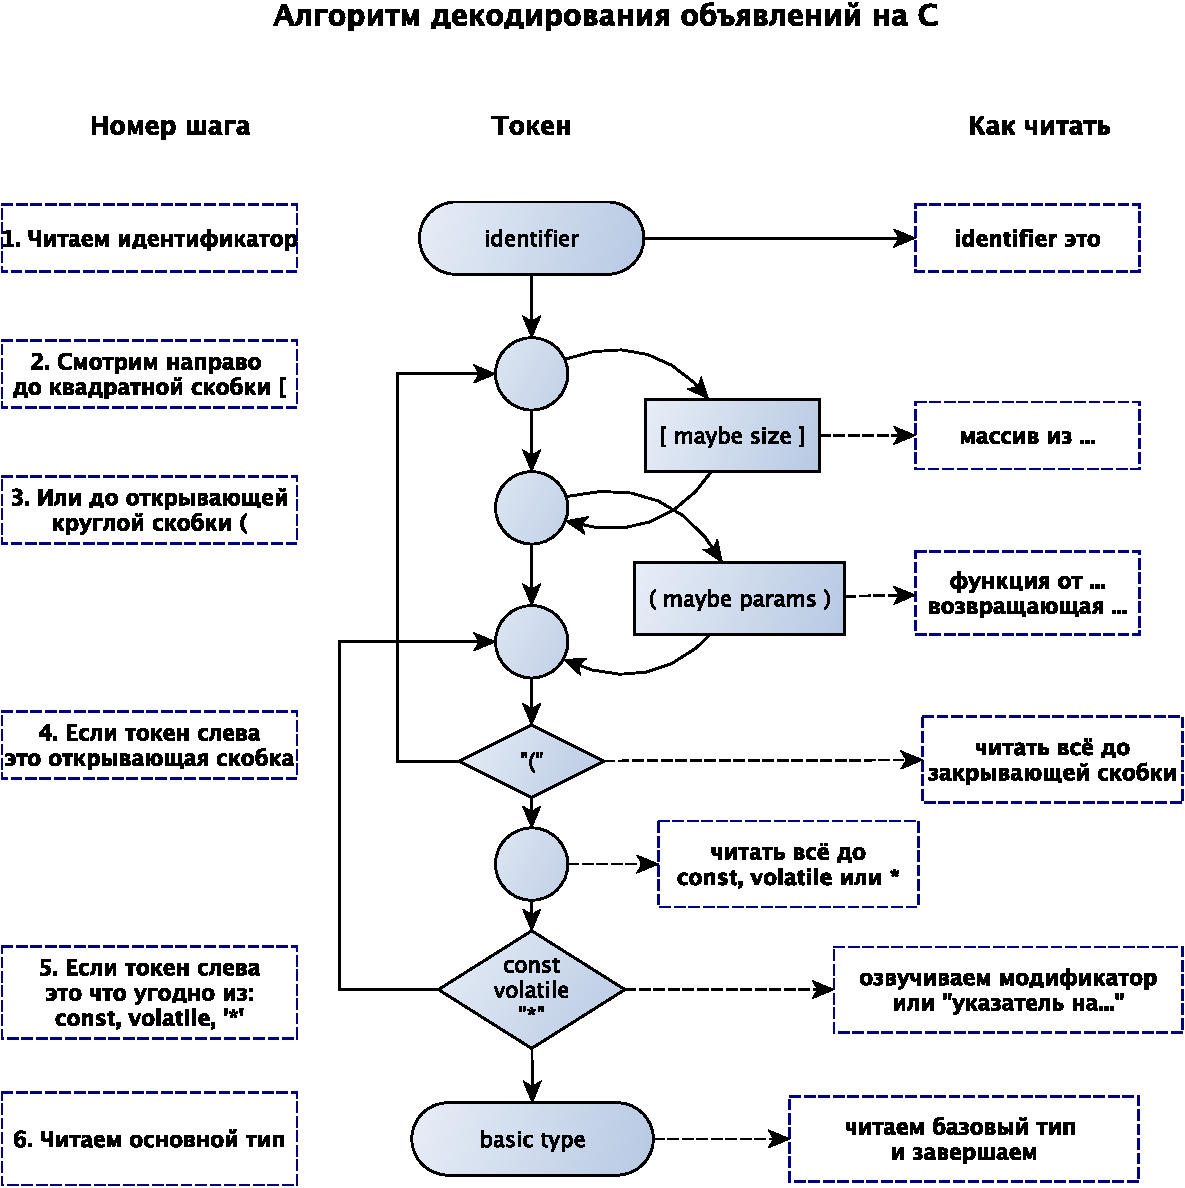
\includegraphics[width=1.0\textwidth]{illustrations/cdecls-crop.pdf}
\caption{Алгоритм разбора объявлений на C}
\label{fig:cdecl_parse}
\end{figure}

\textbf{Домашняя наработка:} по этому алгоритму написать программу, которая парсила бы произвольное объявление на C. Дополнительно: учесть возможность \lstinline!enum!, \lstinline!struct!, \lstinline!union!.

С учётом новых знаний попробуйте прочитать самостоятельно:

\lstinputlisting[firstline=13,lastline=13]{cpp_code/p1s1.cpp}

Ответ: c is array of 10 pointers to functions, accepting pointer to pointer to int and returning pointer to char.

\subsubsection{Ваш друг typedef\index{typedef}}

Рассмотрим прекрасное объявление типа:

\lstinputlisting[firstline=15,lastline=15]{cpp_code/p1s1.cpp}

С помощью \lstinline!typedef! его можно переписать, доставив гораздо меньше боли глазам читающего (и без риска посадить случайную опечатку).

\lstinputlisting[firstline=16,lastline=17]{cpp_code/p1s1.cpp}

Умение читать запутанные объявление не означает необходимости их писать (если вы не участвуете в международном конкурсе по обфускации программ). Где возможно, пользуйтесь \lstinline!typedef!, это хороший стиль. Но ваш личный хороший стиль (с другой стороны) это не основание не иметь навыка чтения запутанных объявлений. Каждый программист в жизни имеет дело с тоннами унаследованного кода, где встречается всякое.

У \lstinline!typedef! есть некоторые опасности, которые часто ускользают от новичков. Так например \lstinline!typedef! может объявить сразу несколько синонимов типов:

\lstinputlisting[firstline=19,lastline=19]{cpp_code/p1s1.cpp}

Это считается дурным тоном, старайтесь этого избегать. Ещё более дурным тоном считается зарыть typedef вглубь объявления, что тоже позволяется синтаксисом.

\lstinputlisting[firstline=20,lastline=20]{cpp_code/p1s1.cpp}

Опытный программист на языке C часто чувствует себя свободнее с препроцессором, скажем вместо

\lstinputlisting[firstline=21,lastline=21]{cpp_code/p1s1.cpp}

Есть соблазн написать

\lstinputlisting[firstline=22,lastline=22]{cpp_code/p1s1.cpp}

Но здесь есть тонкая ловушка:

\lstinputlisting[firstline=21,lastline=25]{cpp_code/p1s1.cpp}

Здесь переменные \lstinline!x! и \lstinline!y! будут разных типов, а \lstinline!w! и \lstinline!v! – одного типа.

\subsection{Знакомство с \lstinline!const!, \lstinline!enum! и \lstinline!inline!}\label{ConstVsDef}

Пример с \lstinline!typedef! показывает нам, что использование возможностей языка лучше, чем использование препроцессора. Есть такие возможности C++, которые кардинально отличают программирование на C-подмножестве C++ и использование которых является хорошим тоном. Например всегда следует предпочитать введение символьных констант препроцессорным объявлениям.

\begin{lstlisting}
#ifdef USE_PREPROC
#define MADELUNGNACL 1.747558
#define PI 3.1415926
#else
const double MADELUNGNACL = 1.747558;
const double PI 3.1415926
#endif

double 
ENaCl (double z, double e, double epsilon, double r)
{
  return (z * e * e * MADELUNGNACL) / (4 * PI * epsilon * r);
}
\end{lstlisting}

Постоянная Маделунга (для определения энергии электростатического взаимодействия одного иона Ei в ионном кристалле) та же самая. Разумеется и $\pi$ то же самое. В чём разница? В первом случае препроцессор сделает текстовую подстановку \lstinline!1.747558! везде, где вы использовали \lstinline!MADELUNGNACL!, во втором случае компилятор объявит (и поместит в таблицу символов для отладочной информации) символьную константу. 

Ещё в большей степени это касается работы с перечислениями (строго говоря, она и в C была введена в C99).

\lstinputlisting[firstline=30,lastline=35]{cpp_code/p1s1.cpp}

Здесь кроме очевидной экономии места, вводится тип keyword, который может принимать только определённые в enum значения, что также является преимуществом.

Ещё сильнее C++ выигрывает для определения небольших функций, где в C были выгодны макросы:

\lstinputlisting[firstline=37,lastline=44]{cpp_code/p1s1.cpp}

Давайте рассмотрим контекст использования

\lstinputlisting[firstline=48,lastline=50]{cpp_code/p1s1.cpp}

Вопрос: что будет содержаться в \lstinline!c! и в \lstinline!d!? А что если подставить вызов функции \lstinline!max!? Ещё лучше объявление функции max будет себя вести при использовании ссылок (мы познакомимся с ними далее).

Кстати, поскольку шаблон раскроется на этапе компиляции, а вызов max почти всегда будет проинлайнен, эффективность C++ метода как минимум не страдает.

Более того, почти всегда, когда в C использовался \lstinline!void*! для передачи параметров неопределённого типа, в C++ можно написать более эффективный код, используя шаблоны. Мы вернемся к этому далее (\ref{CppBetterC}).

\subsection{Различие объявлений и определений\index{declaration}\index{definition}}

До сих пор действия с объявлениями и определениями выполнялись интуитивно, без полного понимания того, что это такое. Давайте теперь посмотрим на детали.

В языке C это довольно просто и это надо просто знать.

Объявление это введение идентификатора и описание типа.

\begin{lstlisting}
extern int bar;
extern int g(int, int);
double f(int, double); /* extern can be omitted for function declarations */
class foo; /* no extern allowed for class declarations */
\end{lstlisting}

Объявление достаточно компилятору, чтобы разрешить ссылки на данный идентификатор.

Определение это реализация типа или выделение памяти объекту.

\begin{lstlisting}
int bar;
int g(int lhs, int rhs) {return lhs*rhs;}
double f(int i, double d) {return i+d;}
class foo {};
\end{lstlisting}

Определение достаточно линкеру, чтобы реализовать идентификатор в объектном коде. 

Объявление может встречаться сколько угодно раз. Определение встречается лишь один раз во всех единицах трансляции на каждую определяемую переменную. Это называется One Definition Rule (ODR\index{ODR}) и оно должно чётко соблюдаться. Нарушение ODR -- UB. При этом определение может заменять собой объявление (т.е. объявление может и не встретится вообще).

Можно запомнить мнемоническое правило чтобы не путать объявление с определением, а в англоязычной литературе declaration и definition, нужно смотреть на словарное упорядочение.  Буква ``б'' расположена раньше, чем ``п''. Значит в словаре слово ``объявление'' будет раньше, чем ``определение'' и так же declaration в английском словаре идёт раньше, чем definition. И так же в программе – объявление всегда должно идти раньше определения.

Важные термины здесь – полный и неполный тип. Если тип (структура, класс, массив) только объявлен, но не определен то этот тип считается неполным. Полным тип  становится только в точке, в которой встречается его определение. Рассмотрим на примере структур.

\lstinputlisting[firstline=57,lastline=65]{cpp_code/p1s1.cpp}

Функция \lstinline!foo! может брать аргументом указатель на \lstinline!t!, но не может брать аргументом сам \lstinline!t! пока тип \lstinline!t! неполный.

Интересно, что строчка одного и того же вида может служит определением или обявлением в зависимости от контекста:

\begin{lstlisting}
typedef void T();
T t; /* declaration of function "t" */

struct X 
{ 
  T t; /* declaration of function "t" */
};

typedef int T;
T t; /* definition of object "t" */
\end{lstlisting}

При рассмотрении шаблонов, станет очевидно, что определения и объявления имеют больше подводных камней, чем описано здесь.

\subsection{Lvalue и rvalue\index{lvalue}\index{rvalue}}

Разговор о C++ невозможен без введения таких фундаментальных понятий, как lvalue и rvalue. Для начала можно рассмотреть пример, который многим из вас может показаться простым.

\begin{lstlisting}
x = y;
\end{lstlisting}

Что здесь написано? Здесь написано – взять адрес переменной x и записать по этому адресу значение переменной y. В этом выражении присваивания, переменная x находится слева, а y справа и стандарт C++98 вводит специальные термины rvalue (right-hand-side value) и lvalue (left-hand-side value) интуитивно понимаемые как ``нечто, что может быть справа (слева) в выражении присваивания''. 

Итак, какие ограничения этот пример накладывает на \lstinline!x!? Похоже, что \lstinline!x! должен быть полного типа, не константым, и иметь определённое местоположение в памяти (быть адресуемым). Есть ли ограничения на \lstinline!y!? Да есть. Он должен быть полного типа и этот тип должен быть совместим с типом \lstinline!x! по присваиванию.  

Это типичный пример того, как компилятор может решить из контекста (в данном случае из положения справа или слева от присваивания) будет ли он использовать адрес переменной или её значение в своих фактических вычислениях. Такая возможность у компилятора есть, потому что адрес переменной полного типа всегда известен во время компиляции и нет необходимости заставлять программиста его специально получать.

\begin{lstlisting}
*(&x) = y;
\end{lstlisting}

Возможно, кстати, писать так было бы честнее. Интересные вещи начинаются, когда дело доходит до массивов и указателей.

\pagebreak
\subsection{Массивы и указатели}

Многие программисты заучивают правило для новичка: массивы в C это указатели и наоборот. Это правило, пожалуй, действительно полезно для новичка. Но в общем случае это не так. Ниже будут проведены чёткие разграничения. Начать следует с указателей. Итак, что можно сделать с указателем (базовые вещи):

\begin{enumerate}
\item Объявить и инициализировать константой
\begin{lstlisting}
int *x = 0;
\end{lstlisting}
\item Объявить и инициализировать адресом переменной или функции
\begin{lstlisting}
struct str_t {int x; int y;};
int foo (int x);
int c = 2;
str_t s = {1, 2};
int *p = &c;
int (*pfoo) (int) = &foo;
str_t *ps = &s;
\end{lstlisting}
\item Присвоить иное значение
\begin{lstlisting}
int bar (int x);
p = x;
x = &c;
pfoo = &bar
\end{lstlisting}
\item Разыменовать и получить или изменить значение
\begin{lstlisting}
c = *x;
*p = 5;
c = (*ps).x;
c = ps->x;
ps->x = *p;
\end{lstlisting}
\item Использовать индексацию, похожую на массив
\begin{lstlisting}
p[0] = c;
*(p+0) = c;
\end{lstlisting}
\item Возвращать из функций
\begin{lstlisting}
int *foo (int x) { return &x; }
\end{lstlisting}
\end{enumerate}

Важно понять: указатели (неконстантные) являются lvalue. В принципе вы можете записать:

\lstinputlisting[firstline=26,lastline=28]{cpp_code/p1s2.cpp}

Этот код является дурным тоном, он будет плохо переносим и совершенно точно тут указатель используется не по назначению, но важно, что это можно сделать. Указатель это честная ячейка памяти. Он хранит то, что туда положил программист.

\begin{figure}[h!]
\centering
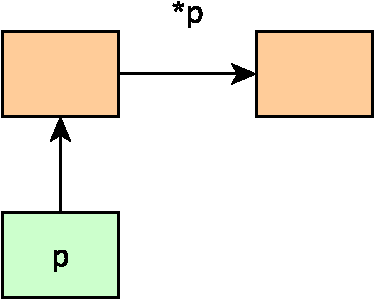
\includegraphics[width=0.3\textwidth]{illustrations/pointers-crop.pdf}
\caption{Визуальное представление указателей}
\label{fig:pointers-crop}
\end{figure}

По аналогии, что можно сделать с массивом

\begin{enumerate}
\item Объявить и инициализировать списком данных (все пропущенные инициализаторы -- нулевые)
\begin{lstlisting}
int a = 5;
int x[10] = {6, a};
\end{lstlisting}
Обратите внимание: неинициализированным может быть только локальный массив. Глобальные массивы всегда инициализированы нулями.
Также обратите внимание. Определение вида:
\begin{lstlisting}
int wrong[]; /* boom! */
\end{lstlisting}
Это ошибка (поскольку компилятор не знает сколько памяти выделять на этот массив). Но мы можем использовать такой синтаксис в объявлениях
\begin{lstlisting}
extern int wrong[]; /* ok */
\end{lstlisting}
\item Прочитать или записать значение
\begin{lstlisting}
int t = x[0];
x[1] = t;
x[0] = x[1];
\end{lstlisting}
\item Деградировать (decay) к указателю если он используется как rvalue
\begin{lstlisting}
int foo (int *t);
int *p = &x[0];
*p = x; /* decay */
a = *(x + 3); /* decay */
a = foo (x + 5); /* decay */
\end{lstlisting}
\end{enumerate}

\begin{figure}[h!]
\centering
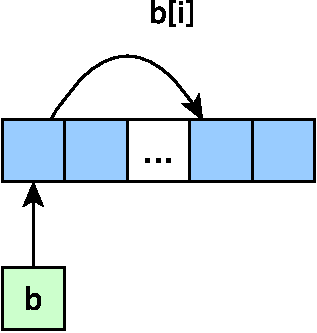
\includegraphics[width=0.3\textwidth]{illustrations/arrays-crop.pdf}
\caption{Визуальное представление массивов}
\label{fig:arrays-crop}
\end{figure}

Но массивы \textbf{никогда} не употребляются вместо указателей там, где указатель это lvalue.

\begin{lstlisting}
int v = 5;
int *p = &v;
int a[1] = {v};
p = a; /* ok */
a = p; /* never */
\end{lstlisting}

По той же причине мы никогда не можем вернуть массив из функции:

\begin{lstlisting}
typedef int arr_t[10];

arr_t foo (void); /* Error! */
\end{lstlisting}

Массивы хранят сами данные, а не указатели на них. То, что они синтаксически могут вырождаться к указателям -- не более, чем причудливый исторический факт, связанный с ранней историей массивов в языке C. Массив содержит lvalue-ячейки данных, но сам как целое он не является lvalue-ячейкой данных.

Кроме того, инициализация массивов и указателей выглядит похоже, но означает разные вещи:

\lstinputlisting[firstline=35,lastline=37]{cpp_code/p1s2.cpp}

Вопрос: есть ли разница между этими двумя записями и какую вы предпочтёте? Почему?

Верный ответ: строчка 1 предпочтительней, чем (устаревшая, с Wall + Werror выдаст ``error: deprecated conversion from string constant to \lstinline!char*!'') строчка 2 и они имеют разную семантику. Память под массивы выделяется автоматически (и строчка 1 подразумевает неявный memset) но память никогда автоматически не выделяется под указатели, поэтому для построения динамических структур данных (например, связных списков) используются указатели, а не массивы.

Между прочим, строковые литералы в инициализации указателей это счастливое (и опять таки исторически сложившееся) исключение. Строчка 2 в примере ниже:

\lstinputlisting[firstline=43,lastline=44]{cpp_code/p1s2.cpp}

Не будет скомпилирована.

Вопрос: есть ли разница между

\begin{lstlisting}
int foo (int x[]);
int foo (int *x);
\end{lstlisting}

Ответ: из-за decaying разницы нет.

Вопрос: означает ли эта запись:

\begin{lstlisting}
int foo (int x[16]);
\end{lstlisting}

Что \lstinline!foo! принимает массив из 16 символов?

Ответ: нет, здесь \lstinline!foo! принимает любой указатель.

Но это всё были одномерные случаи. Что же с многомерными массивами?

\subsubsection{Многомерные массивы\index{multidimensional arrays}}

Язык C и C-подмножество языка C++ не поддерживают семантику ``настоящего'' многомерного массива на уровне языка.  То, что поддерживается, является по факту ``массивом массивов ... массивов''. 

К ним применяются те же правила, что к обычным массивам, например

\lstinputlisting[firstline=60,lastline=60]{cpp_code/p1s2.cpp}

Причём последние индексы идут последними. Так же и с инициализацией:

\lstinputlisting[firstline=63,lastline=63]{cpp_code/p1s2.cpp}

Причём наиболее вложенные скобки относятся к последним индексам. Первый индекс ясен из контекста и его можно опускать в инициализаторе.

Если часть вложенных инициализаторов пропущена, они считаются нулевыми, поэтому, например двумерные массивы символов могут быть проинициализированы последовательностями строковых литералов.

При передаче многомерных массивов в функции может быть опущен только первый индекс в прототипе (и он может быть любым). Остальные индексы у формального и фактического аргументов должны совпадать.

Вот такой прототип функции не может быть скомпилирован

\begin{lstlisting}
int func(int a[][], int n);
\end{lstlisting}

Это происходит потому, что массивы в памяти должны занимать непрерывную память. Для многомерных массивов раскладка в памяти идёт построчно

\begin{lstlisting}
int a[2][3];
/* TODO: картинка */
/* a[0][0], a[0][1], a[0][2], a[1][0], ... */
\end{lstlisting}

Дальше когда встречается индексирование \lstinline!a[i][j]!, компилятор генерирует код \lstinline!*(a + i*3 + j)!
Но, чтобы сгенерировать такой код, компилятор должен знать все измерения, кроме первого. Именно поэтому чтобы передать многомерный массив, программист должен так или иначе сообщить эту информацию компилятору.

\begin{lstlisting}
int func(int a[][3], int n);
int func(int (*a)[3], int n);
\end{lstlisting}

Некоторые думают, что можно обойтись двойным указателем.

\begin{lstlisting}
int func(int **a, int n, int m);
int a[2][3];
func (a, 2, 3); /* wrong! */
\end{lstlisting}

Но это не работает. Двумерный массив уже не может деградировать к указателю на указатель, а только к указателю на массив. Забавный хак в этом отношении -- обойтись одинарным указателем:

\begin{lstlisting}
int func(int *a, int n, int m);
int a[2][3];
func (&a[0][0], 2, 3); /* ok */
\end{lstlisting}

Но внутри функции это потребует ручного обслуживания такого "развернутого" массива.

Точно так же нельзя, даже указав нужные инициализаторы, определить двумерный массив, для которого компилятор дедуцирует оба размера

\begin{lstlisting}
int a[][] = {{1, 2}, {3, 4}}; /* Error! */
\end{lstlisting}

Увы, но здесь, как и в прототипах функций, должны быть указаны все размеры, кроме, может быть, первого.

\subsection{От указателей к ссылкам\index{references}}

Очень важной особенностью C++ является введение довольно низкоуровневой, но принципиально новой конструкции – ссылок. Ссылка это альтернативное имя переменной.

\lstinputlisting[firstline=67,lastline=70]{cpp_code/p1s2.cpp}

Каждая ссылка обязательно должна быть инициализирована в точке определения. ``Ссылка сама по себе'' так же как ``нулевая ссылка'' не могут существовать. Указатель сам по себе является местом для хранения данных, ссылка – это просто имя. Поэтому ссылки не нуждаются в явном разыменовании – каждое обращение к ним это уже разыменование. Поэтому различия существенны:

\lstinputlisting[firstline=76,lastline=81]{cpp_code/p1s2.cpp}

\subsubsection{Когда ссылки уступают указателям}

В целом при программировании на C++ следует повсюду предпочитать использование ссылок использованию указателей.

Но есть нюансы. Ссылки иммутабельны -- назначив ссылку ``другим именем'' чего-то, её нельзя перевязать на что-то другое

\begin{lstlisting}
int a = 2;
int b = 3;

int *pa = &a; /* ok */
pa = &b; /* ok, now *pa == 3 */

int &ra = a; /* ok */
ra = b; /* ok, now a == 3 */
\end{lstlisting}

Вторая строчка в случае ссылок -- не перевязывает ссылку, а присваивает значение тому lvalue на которое она ссылается. Поэтому ссылки нельзя использовать для создания динамических структур данных (см. ниже про динамическую память) таких как стеки, очереди, деревья.

Кроме того, у ссылок нет аналога \lstinline!(void *)! для передачи идиомы ``ссылки на неопределённый тип''. Появившиеся в новом стандарте \lstinline!auto&! всё таки должны быть разрешены на этапе компиляции, что бывает невозможно:

\begin{lstlisting}
void *read (void);

void 
use (void)
{
  int a = *(int *) read(); /* read int */
  double d = *(double *) read(); /* next read double */
  /* ... */
}
\end{lstlisting}

Итак, использование ссылок должно происходить где это возможно, но нужно хорошо понимать места, в которых их использование невозможно или нецелесообразно.

\subsection{От malloc и free к new и delete\index{new}\index{delete}\label{newdelete}}

Для управления динамической памятью в языке C использовались библиотечные функции malloc и free. Они остались в C++, но их использование не рекомендовано и считается дурным тоном, поскольку C++ предоставляет гораздо более гибкие возможности с помощью ключевых слов \lstinline!new!, \lstinline!delete! и \lstinline!delete[]!.

\lstinputlisting[firstline=87,lastline=90]{cpp_code/p1s2.cpp}

Следует оговориться, что для C-подмножества эти возможности пожалуй менее гибкие и более ограничивающие. Нужно помнить о парности \lstinline!new!/\lstinline!delete! и \lstinline!new a[]!/\lstinline!delete[] a! и нет возможности сделать \lstinline!realloc!. Вся сила новых ключевых слов раскроется позже, когда будут рассматриваться элементы ООП. Пока что вы можете просто запомнить их и начинать применять. Впрочем и в C-подмножестве можно найти плюсы.

Например \lstinline!new! существенно упрощает выделение в памяти многомерных массивов, что было не так то просто в случае языка C. Для C++ можно просто записать:

\begin{lstlisting}
typedef int dimensions[3][4];

dimensions * dim = new dimensions[10];
dim[/* from 0 to 9 */][/* from 0 to 2 */][/* from 0 to 3 */] = 42;
delete [] dim;
\end{lstlisting}

Это не требует убогих трюков когда массив выделяется как одномерный, а потом обслуживается как двумерный -- всё прозрачно и типизировано.

\subsection{От приведения в стиле C к приведению в стиле C++\index{cast}}

Язык C, поскольку он разрабатывался с интенцией отображения один в один на машинные типы, имеет слабую типизацию. Кусок памяти, который хранит int или указатель на int или механическую структуру из чего-нибудь, легко приводится к другому такому же куску памяти.

\lstinputlisting[firstline=95,lastline=100]{cpp_code/p1s2.cpp}

Язык C++ содержит гораздо более развитую систему типов и позволяет определять типы, обладающие состоянием и поведением, о которых пойдёт речь в следующих лекциях. Поэтому, несмотря на то, что формально C++ унаследовал от C способ непосредственного приведения C-style cast, применять его считается крайне плохим тоном. Вместо этого следует применять \lstinline!static_cast!\index{static\_cast}, \lstinline!reinterpret_cast!\index{reinterpret\_cast} или \lstinline!const_cast!\index{const\_cast}. Чаще всего вы будете применять \lstinline!static_cast!. Он записывается так:

\lstinputlisting[firstline=106,lastline=107]{cpp_code/p1s2.cpp}

В принципе это ничем не отличается от C-стиля, рассмотренного выше. Запись чуть более уродлива, зато чуть лучше бросается в глаза в коде программы. Разница в том к чему можно применять \lstinline!static_cast!, а к чему C-cast. Последний применяется к чему угодно. \lstinline!static_cast! применяется только к переменным, совместимым по статическим типам. Его можно использовать в преобразовании \lstinline!int*! к \lstinline!float*! (и то и другое – указатели). 

Гораздо более редкий \lstinline!const_cast! нужен для снятия константности и волатильности. С его помощью можно привести \lstinline!const int *! к \lstinline!int *!. 

\lstinputlisting[firstline=113,lastline=114]{cpp_code/p1s2.cpp}

Вы конечно понимаете опасность этих игр – в памяти, выделенной для \lstinline!const int*!, компилятор размещает данные, изменения которых не ожидает. В тот момент, когда вы принудительно снимаете константность и изменяете (пытаетесь изменить) нечто объявленное ранее константным, вы стреляете себе в ногу.

И самый редкий \lstinline!reinterpret_cast! существует для непереносимых низкоуровневых приведений, которые, тем не менее, иногда нужны.

\lstinputlisting[firstline=120,lastline=121]{cpp_code/p1s2.cpp}

Любое использование \lstinline!reinterpret_cast! (как и C-cast) компрометирует вашу программу. Но случаи использования \lstinline!reinterpret_cast! читающему ваш код будет куда проще найти и вычистить.

Выучить и использовать эти три оператора не намного сложнее, чем использовать обычные преобразования в стиле C, но в дальнейшем они сослужат вам отличную службу, упрощая поддержку кода и не давая посадить тяжело обнаружимых ошибок приведения.

\subsection{Перегрузка функций, аргументы по умолчанию и искажение имён\index{Function Overloading}\index{Name Mangling}}\label{NameResolution}

Вопрос к слушателям сколько функций вычисления квадратного корня вы можете назвать из стандартной библиотеки языка C?

Правильный ответ: три (7.12.7.5) \lstinline!sqrtf!, \lstinline!sqrt! и \lstinline!sqrtl!. Три функции с разными именами понадобилось вводить потому, что они принимают аргументы разных типов, а язык C предоставляет достаточно сильную гарантию того, что любое имя, использованное в вашей программе будет отображено в ассемблер вашей целевой машины один к одному, без искажения.

Язык C++ такой гарантии не даёт. Вместо этого он согласен сделать эту (и многую другую) работу за вас посредством встроенного искажения (манглирования) имён. Используя C++ вы можете написать три функции с одинаковыми именами, но различными типами:

\lstinputlisting[firstline=125,lastline=127]{cpp_code/p1s2.cpp}

Посмотрим во что они были откомпилированы в ассемблер:

\begin{lstlisting}[language=make]
_Z3fooc:
...
_Z3fooi:
...
_Z3foox:
...
\end{lstlisting}

Конвенции манглирования не документированы и являются implementation-defined, закладываться на них не надо. Но грамотно использовать механизм перегрузки функций в C++ бывает очень выгодно для облегчения читаемости вашей программы.

Иногда требуется из кода на C++ сделать некую функцию или переменную (обычно входящую в интерфейс модуля) ``линкуемой в C стиле'' -- т.е. отображаемой в ассемблер один в один. Для этого используется \lstinline!extern "C"!

\begin{lstlisting}
extern "C" void 
foo(int);

extern "C"
{
   void g(char);
   int i;
}
\end{lstlisting}

Так слинкованы могут быть функции и переменные, но не члены классов. Две функции с такой линковкой с одинаковым именем -- нарушение ODR.

\textbf{Домашняя наработка:} посмотрите как работает манглирование в вашем любимом компиляторе. Можете ли вы установить некие закономерности?

Также удобная концепция (и снова проистекающая от отсутствия обязательств C++ быть близким к машине) это аргументы по умолчанию. Посмотрим как они могут быть заданы:

\lstinputlisting[firstline=1,lastline=5]{cpp_code/p1s2.cpp}

Функция не может быть перегружена по значению аргумента по умолчанию. Для перегрузки вы можете использовать только сигнатуру – возвращаемый тип функции и типы её аргументов.

Перегрузка функций и аргументы по умолчанию сильно упрощают работу с именами функций в C++, перенося всю её тяжесть на плечи компилятора и вам следует научиться использовать эти возможности правильно.

\subsubsection{Правила разрешения перегрузки\index{overloading resolution}}

Многие считают, что разрешение перегрузки в C++ неочевидно и подчиняется странным правилам. На самом деле это так и есть. Но вдумчивое чтение стандарта (вся 13 глава посвящена перегрузке) позволяет вывести некоторые закономерности. 

Можно запомнить или записать:

Если среди вариантов перегрузки присутствует функция, точно совпадающая с вызываемой по типам аргументов, будет вызвана она. Далее применяются преобразования аргументов в следующем порядке:

\begin{enumerate}
\item Стандартные преобразования
\item Пользовательские преобразования
\item Троеточия
\item Ссылочное связывание
\item (новый стандарт) Списочная инициализация
\end{enumerate}

После каждого типа преобразований сверху-вниз, получается множество возможных функций. Если это множество состоит из одной функции, будет вызвана она. Если это множество состоит из нескольких функций, будет выдана ошибка компиляции. Если это множество пусто, будет попробован следующий тип преобразований аргументов.

Пока можно оставить за бортом третий и пятый типы преобразований, до них дойдёт дело в своё время. Простой пример на всё остальное:

\begin{lstlisting}
#include <cstdio>

int foo (char x) { return 0;}  /* step 1 */
int foo (short x) { return 1;} /* step 1 */
int foo (int x) { return 2;}   /* step 0 */
int foo (...) { return 3;}     /* step 3 */
int foo (int &x) { return 4;}  /* step 4 */

int
main (void)
{
  std::printf ("result: %d\n", foo (10));
  return 0;
}
\end{lstlisting}

Здесь никаких конфликтов нет. Для вызова \lstinline!foo (10)! точно подходит \lstinline!foo (int)!, программа возвращает 2.
Если стереть её, то будет ошибка компиляции:

\begin{lstlisting}
#include <cstdio>

int foo (char x) { return 0;}  /* step 1 */
int foo (short x) { return 1;} /* step 1 */
int foo (...) { return 3;}     /* step 3 */
int foo (int &x) { return 4;}  /* step 4 */

int
main (void)
{
  std::printf ("result: %d\n", foo (10));
  return 0;
}
\end{lstlisting}

Конфликт между двумя равноправными функциями \lstinline!step 1!. Если далее стереть одну из них:

\begin{lstlisting}
#include <cstdio>

int foo (char x) { return 0;}  /* step 1 */
int foo (...) { return 3;}     /* step 3 */
int foo (int &x) { return 4;}  /* step 4 */

int
main (void)
{
  std::printf ("result: %d\n", foo (10));
  return 0;
}
\end{lstlisting}

Снова всё норм, программа вернёт 0. Если стереть оставшуюся.

\begin{lstlisting}
#include <cstdio>

int foo (...) { return 3;}     /* step 3 */
int foo (int &x) { return 4;}  /* step 4 */

int
main (void)
{
  std::printf ("result: %d\n", foo (10));
  return 0;
}
\end{lstlisting}

Программа вернёт 3. И, наконец, если стереть все варианты кроме ссылочного связывания, программа вернёт 4.

Если вдуматься в эти правила они уже не выглядят столь марсианскими, правда? Хех. Это от того, что я рассказал вам их \textbf{не все}. Тема разрешения перегрузок ещё будет затронута в разговоре про ООП и далее, в разговоре про новый стандарт. Но на уровне C подмножества, всё выглядит довольно логично.

\subsection{Пространства имён, using и поиск Кёнига\index{namespaces}}

Каждое объявление в C++ принадлежит некоторому пространству имён. Глобальное пространство имён это префикс через два двоеточия, а все стандартные функции принадлежат пространству имён std. Напишем hello world с явным указанием пространств имён.

\lstinputlisting[firstline=1,lastline=7]{cpp_code/p1s3.cpp}

Обратите внимание на включение \lstinline!<cstdio>! вместо привычного \lstinline!<stdio.h>! хедера. Все заголовочные файлы к которым вы привыкли в C, сохранены в C++. Но хорошим тоном считается писать унаследованные заголовочные файлы в C++ conforming виде, то есть \lstinline!<cXXX>! вместо \lstinline!<XXX.h>!.

Засорять собственными именами, такими как \lstinline!::helloworld!, глобальное пространство имён это на самом деле крайне плохая идея. Несколько лучше объявить своё пространство имён, включив туда всё, что специфично именно для вашей программы.

\lstinputlisting[firstline=1,lastline=9]{cpp_code/p1s4.cpp}

Допустимо объявлять вложенные пространства имён с произвольным количеством уровней вложенности. При помещении в пространство имён функции с большим телом, вполне достаточно поместить в пространство имён явно только объявление (например в заголовочном файле), указав пространство имён при определении (например в файле реализации).

\lstinputlisting[firstline=1,lastline=6]{cpp_code/p1s5.cpp}

Пространства имён являются областями видимости (как блоки из фигурных скобок) и подчиняются тем же правилам – если имя указано в охватывающем пространстве имён оно может быть использовано без квалификации. Но в отличии от блоков скобок они могут быть поименованы и тогда переменная или функция с квалификацией может быть использована где угодно

\lstinputlisting[firstline=8,lastline=17]{cpp_code/p1s5.cpp}

Здесь приведён пример неименованного пространства имён (по русски это звучит странно, мы будем часто говорить ``анонимное пространство имён''). В пространстве имён buz у нас нет доступа к y, объявленному в анонимном пространстве имён, зато есть доступ к \lstinline!foo::y!. Также можно избежать необходимости постоянно ставить некий префикс (скажем std) если включить это пространство имён в текущее с помощью директивы using. Этой директивой можно включить и одно имя и целое пространство.

Когда компилятор видит, например, вызов функции, имя этой функции он будет искать:
\begin{itemize}
\item
сначала в области видимости вызова и текущем пространстве имён
\item
далее в пространствах имён аргументов, включая их классы и все базовые классы
\end{itemize}

Этот трюк называется ``поиск Кёнига''\index{Kenig search} по имени человека, который его придумал и ввёл в стандарт C++98.

\lstinputlisting[firstline=19,lastline=28]{cpp_code/p1s5.cpp}

Впрочем, если компилятор встречает вызов фукции из функции-члена некоего класса, то иные члены этого класса и его родительских имеют приоритет над функциями, найденными на основании информации о типах аргументов.

Любая стандартная функция в C++ принадлежит пространству имён std. Каждый раз писать \lstinline!std::printf! или \lstinline!std::memcpy! бывает накладно. Чтобы этого избежать, добавьте строчку \lstinline!using namespace std!\index{using} после включения хедеров. Директива \lstinline!using some_name! также может применяться чтобы внести из произвольного пространства имён только одно имя.

\lstinputlisting[firstline=1,lastline=10]{cpp_code/p1s6.cpp}

Все правила для пространств имён нужно хорошо знать и ещё раз освежить в стандарте по мере того, как вы забудете то, о чём я говорил здесь.

\subsection{Мелкие отличия C-подмножества C++ от ANSI C}

\begin{itemize}
\item
Функция \lstinline!main()! в C++ не может быть вызвана из пользовательского кода. В языке C это разрешено, хотя и несколько необычно.
\item
Прототипы функций обязательны в C++, но опциональны в C.
\item
Сложная и развитая система инициализации в C обычно не работает в C++

\begin{lstlisting}
struct T {
    union {
        struct {
            int x, y, z;
        };
        int xyz[3];
    };
    int a;
};

struct T v = { { .x = 1, .y = 2, .z = 3}, 4 };
struct T w = { { .xyz[0] = 1, .xyz[1] = 2, .xyz[2] = 3}, 4 };
struct T x[] = { [0].a = 1, [1].a = 2 };
\end{lstlisting}

Такой код инициализации легален в C и совершенно нелегален в C++
\item
Имена, определяемые через \lstinline!typedef! не могут совпадать с существующими именами структур в C++, но могут в C (последний требует явной квалификации \lstinline!struct!).
\item
При присвоении к \lstinline!void *! указателю указателя на иной тип, C++ требует приведения (C не требует, но оно считается хорошим тоном).
\item
C++ вводит более десяти новых ключевых слов. Они могут быть использованы как идентификаторы в программе на C, но компилятор C++ выдаст ошибку.
\item
В языке C++ объявление переменной может появится везде, где может быть выражение; в C, объявления должны быть в начале блока.
\item
Имя структуры или объединения во внутренней области видимости скроет такое же имя любой переменной во внешней области видимости в C++, но не в C.
\item
У символьных литералов тип char в C++, но тип int в C. То есть \lstinline!sizeof('a')! даёт 1 в C++, но может дать большее значение в C.
\end{itemize}

\pagebreak
\subsection{Домашняя наработка по второй части}
\begin{enumerate}
\item
Дана структура данных, воплощающая простой односвязный список

\begin{lstlisting}
typedef struct list_tag
{
  void *data;
  struct list_tag *next;
} list_t, *list_p;
\end{lstlisting}

У последнего элемента \lstinline!next = 0!

Необходимо написать на языке C++ функцию, берущую на вход указатель на голову списка и переворачивающую список в памяти, так, что первый элемент становится последним, второй предпоследним и так далее.

\item
Дана программа на языке C с комментариями вида \lstinline!/* comment */!

Необходимо написать на языке C++ программу, выкидывающую все комментарии из текста данной.

\item
Дана структура данных, соответствующая n-арному дереву

\begin{lstlisting}
typedef struct tree_tag
{
  void *data;
  struct tree_tag *top;
  struct tree_tag **childs;
} tree_t, *tree_p;
\end{lstlisting}

Реализуйте на языке C++ функцию, берущую на вход пару указателей на произвольные элементы дерева, и подсчитывающую расстояние между ними (минимальный путь в дереве). Как вы будете тестировать эту функцию?

\item
Реализуйте на языке C++ алгоритм из (\ref{AlgDecl}) и протестируйте на нескольких сотнях сгенерированных определений

\item
Реализуйте на языке C++ транспонирование двумерной матрицы

\item
Реализуйте на языке C++ операцию получения двумерной матрицы обратной данной

\item
Реализуйте на языке C++ операцию умножения вектора на матрицу

\item
Реализуйте на языке C++ калькулятор считающий в обратной польской нотации. Например \lstinline!1 2 3 4 + * + =! должно выдавать 25 в качестве результата.

\item
Известны год, месяц и день рождения человека. Реализуйте на языке C++ программу, определяющую его возраст в днях на текущую дату.

\item
Реализуйте на языке C++ программу, подсчитывающую количество лет в 20-м веке у которых первым днём было воскресенье

\item
На вход дана строка из \lstinline!N*N! символов. Реализуйте на языке C++ функцию, выделяющую в памяти двумерную матрицу \lstinline!N*N! и заполняющую её последовательными данными из входной строки.

\item
На вход даны завершающаяся нулём строка \lstinline!haystack! и завершающаяся нулём строка \lstinline!needle!. Реализуйте на языке C++ функцию, определяющую, является ли \lstinline!needle! подстрокой \lstinline!haystack!

\item
В условиях предыдущей задачи необходимо доработать функцию, чтобы она выкидывала из \lstinline!haystack! все вхождения \lstinline!needle! и возвращала измененную строку.

\item
Напишите на C++ программу, которая будет возвращать номер в последовательности Фибоначчи первого числа имеющего 1000 разрядов в десятичном представлении.

\end{enumerate}

\pagebreak
\section{Объектно-ориентированное счастье}

Как известно самой целью создания C++ Бьёрном Строструпом было добавление ОО-возможностей к C, поэтому изначально язык назывался ``C с классами''. Известно что Строструп вдохновлялся языком Simula, но сейчас уже нельзя оценить насколько это была удачная идея, поскольку этот язык канул в лету. С другой стороны, известному гуру ООП, Кенту Беку, приписывается высказывание: ``Это я придумал термин \textit{объектно-ориентированный} и я не имел в виду C++''. Так или иначе, но C++ действительно обладает уникальной среди современных ОО-языков моделью объявления и инстанциирования классов. Многим нравится богатство и гибкость её возможностей, многие в ужасе отползают. Впрочем, давайте начнём с основ.

\subsection{Структуры в C и в C++, POD и NPOD\index{POD}\index{NPOD}}

В языке C структура являлась способом ввести пользовательский тип, являющийся механическим объединением разнородных данных:

\lstinputlisting[firstline=1,lastline=12]{cpp_code/p2s1.cpp}

Такие типы возможны и в C++ и они называются POD-типами (от английского Plain Old Data). Но в C++ была также добавлена принципиально новая возможность группировать данные с методами их обработки внутри структуры:

\lstinputlisting[firstline=1,lastline=13]{cpp_code/p2s2.cpp}

Получившийся тип (собственно ``not POD-тип'' или ``NPOD-тип'') несколько удобнее в работе. Но при этом теряются гарантии по расположению в памяти и размерам (которые с учётом выравнивания и в C в общем-то были довольно призрачными). Обратите внимание что в C++ была исключена необходимость добавлять struct к символьному имени структуры, что делает ненужным оставшийся в C-style коде typedef тэга структуры на её имя.

Кстати имя метода \lstinline!transpose_pair! структуры \lstinline!pair_t! в C++ также будет манглировано (вспоминаем прошлую лекцию) и в ассемблере встретится, например в виде:

\begin{lstlisting}[language=make]
_Z14transpose_pair4pair:
\end{lstlisting}

Определённая так функция называется методом. Объявление метода происходит внутри определения структуры, определение метода имеет явную квалификацию того к чему метод относится. Обратите внимание, что символ сдвоенных двоеточий такой же, как и в случае пространств имён. Он дословно означает пространство имён, задаваемое структурой.

Использование \lstinline!this! внутри метода позволяет получить данные той структуры, для которой метод был вызван, так что нам не надо специфицировать исходную структуру как параметр. Его использование можно опустить.

\subsection{Инкапсуляция и игра в мячик}

Представим, что вас попросили разработать тип данных, который будет использован для моделирования полёта материальной точки в двумерном мире (высота, длина). Мяч может лететь свободно, для чего у него вызывается метод \lstinline!fly(double t)! или его можно толкнуть, придав ему определённую скорость под определённым углом (после чего например опять отправить в полёт и так далее). Вы напишете нечто вроде:

\lstinputlisting[firstline=14,lastline=23]{cpp_code/p2s1.cpp}

Представляет ли эта структура данных абстракцию мяча, о которой вас просили? Нет, не представляет. Каждый пользователь вашего ``мяча'' может произвольно менять его координаты. Это означает, что в плохо отлаженной программе симуляции, ваш мяч сможет свободно ``телепортироваться'', а это явно не то, чего ждут от законченной модели. 

\lstinputlisting[firstline=29,lastline=36]{cpp_code/p2s1.cpp}

Хуже того, время может быть свободно переставлено вперёд или назад. Но пусть даже никто не ошибся и всё написано правильно. А потом... возникла необходимость ``запустить'' ваш мяч в многопользовательской среде. Всё пропало – для того, чтобы вставить синхронизацию, переписывать придётся каждый участок кода где ссылались на эти поля.

\subsubsection{Конкретные классы}

Для разграничения состояния модели от её поведения и более гибкого управления поведением, в C++ были введены классы. Простые классы, без использования полиморфизма и без иерархий наследования, называются ``конкретными классами''. Конкретные классы -- мощный и полезный инструмент для поддержания консистентности абстракции. Перепишем модель мяча, создав его класс

\lstinputlisting[firstline=43,lastline=54]{cpp_code/p2s1.cpp}

Модификатор \lstinline!public! означает, что любой пользователь типа \lstinline!ball_t! имеет доступ к этим методам или данным. 

Модификатор \lstinline!private! означает, что доступ к соответствующим методам и данным имеют только методы этого класса.

\lstinputlisting[firstline=58,lastline=74]{cpp_code/p2s1.cpp}

Хорошим тоном считается закрывать данные, составляющие состояние объекта и открывать функции, составляющие его поведение.

Обратите внимание на опущенный \lstinline!this! в коде \lstinline!ball_t::push!, это допустимо.

\subsubsection{Инициализация и уничтожение\index{constructor}\index{destructor}}

Отсутствие доступа к состоянию означает, что при создании объекта он должен уметь сам установить своё состояние, а при уничтожении – освободить свои ресурсы. Для этого в класс вводятся конструктор и деструктор – специальные функции, вызывающиеся при создании и уничтожении объекта. Например у класса мяча, конструктор может устанавливать начальное положение, деструктор же может быть тривиальным.

\lstinputlisting[firstline=18,lastline=21]{cpp_code/p2s2.cpp}

Обратите внимание на список инициализации у конструктора в этом примере кода. Можно, конечно, написать инициализацию в теле конструктора, но использование списков инициализации является лучшей идеей. По умолчанию, удовлетворяющий стандарту языка C++ компилятор позаботится о вас, сгенерировав вам конструктор и деструктор по умолчанию (позднее мы поговорим о степени этой заботы и её оборотных сторонах). Конструктор по умолчанию вызывает конструкторы всех членов класса, у которых они есть, деструктор -- их деструкторы.

Важная тема в конструкторах это их использование для задания неявного преобразования типа\index{implicit type cast}. Неявные преобразования есть и в C, там они называются type promotions, некоторые из них (действуют и в C++) сведены в таблицу ниже (здесь anytype это любой встроенный тип, совместимый по операции но не перечисленный выше):

\begin{lstlisting}
anytype `op` long double => long double `op` long double
anytype `op` double => double `op` double
anytype `op` float => float `op` float
anytype `op` unsigned long long => unsigned long long `op` unsigned long long
anytype `op` long long => long long `op` long long
anytype `op` unsigned long => unsigned long `op` unsigned long
anytype `op` long => long `op` long
anytype `op` unsigned int => unsigned int `op` unsigned int
anytype `op` int => int `op` int
\end{lstlisting}

Но в C++ неявные преобразования также пробуются компилятором для пользовательских типов. Определение в пользовательском типе конструктора, который может быть истрактован как конструктор с одним аргументом (считая аргументы по умолчанию частично подставленными всюду кроме первого аргумента), считается определением неявного преобразование из аргумента конструктора к этому типу. Это может иметь неприятные последствия:

\lstinputlisting[firstline=26,lastline=31]{cpp_code/p2s2.cpp}

Верный способ определить конструктор, чтобы явно заявить компилятору, что он не поддерживает неявного преобразования это определить его с ключевым словом explicit

\lstinputlisting[firstline=12,lastline=13]{cpp_code/p2s3.cpp}

Это важное решение при проектировании и его надо принимать осознанно. Лепить explicit куда ни попадя -- дурной тон (скажем это ключевое слово возможно но совершенно не нужно на конструкторе более чем с одним аргументом и без аргументов по умолчанию). Но иногда он очень нужен.

\subsubsection{Селекторы}

Отражает ли созданная до сих пор абстракция физический мяч? Всё ещё нет. Мяч в физическом мире обычно виден пользователю, у которого есть возможность считать его координаты. То есть нам нужны некоторые методы, которые будут, сохраняя состояние мяча, давать возможность прочитать его. Такие методы традиционно называются селекторами.

\lstinputlisting[firstline=16,lastline=18]{cpp_code/p2s3.cpp}

Обратите внимание на const в их объявлении. Внутри объявленного таким образом метода изменить любое поле класса это ошибка компиляции. Исключение составляют поля, объявленные с mutable.

Хорошим тоном является делать селектором любой метод, который теоретически может быть селектором и по логике не должен менять внутреннего состояния объекта.

\subsubsection{Статические константы в классе\index{static members}}

Задумаемся над реализацией метода fly. Очевидно, нам понадобится ускорение свободного падения. Логично сделать его константой общей для каждого экземпляра класса \lstinline!ball_t!, но при этом закрытой, так как это его деталь реализации.

Пишем объявление:

\lstinputlisting[firstline=9,lastline=9]{cpp_code/p2s3.cpp}

Определяем вне определения класса:

\lstinputlisting[firstline=26,lastline=26]{cpp_code/p2s3.cpp}

И теперь можно написать код полёта:

\lstinputlisting[firstline=35,lastline=42]{cpp_code/p2s3.cpp}

И мяч полетит. 

Вообще спецификатор \lstinline!static! в классах используется для объявления статических членов, то есть таких атрибутов и методов, которые являются методами и атрибутами класса, а не объекта. Подобно константе \textbf{g}, все статические члены которые нуждаются в инициализации должны быть определены вне определения класса.

\subsubsection{Объявления и определения классов}

Это важный момент, перекликающийся с затронутой на прошлой лекции темой объявлений и определений. Объявление класса как неполного типа выглядит так:

\begin{lstlisting}
class ball_t;
\end{lstlisting}

С этого момента тип \lstinline!ball_t! можно использовать по правилам, прописанным в стандарте для неполных типов. Определение класса это объявление всех его методов и полей.

Но внутри определения класса, каждое объявление поля, статического поля или метода это его объявление. Определением нестатического члена считается конструктор класса (поэтому если членом класса является ссылка она должна быть инициализирована в списке инициализации конструктора). Определение метода может как встречаться внутри класса, так и быть вынесено вне его. Определение статического объекта всегда должно быть вне класса.

Давайте сведём всё воедино.

\subsubsection{Игра в мячик (код)}\label{BallGame}

\lstinputlisting{cpp_code/p2s3.cpp}

\subsection{Классы для управления ресурсами, идиома RAII\index{RAII}}\label{RAII}

При программировании на языке C часто возникает проблема освобождения занятых ресурсов. Ресурс это нечто, что ваша программа может использовать, но при этом должна вернуть системе, иначе могут возникнуть неприятности. Самым частым примером ресурса является динамическая память.

Вопрос студентам: какие ещё вы знаете ресурсы.

Ожидаемые ответы: файловые дескрипторы, мьютексы, шрифты и кисти, объекты гуя, соединения с бд, сокеты.

Рассмотрим пример файлового дескриптора.

\lstinputlisting[firstline=11,lastline=39]{cpp_code/p2s4.cpp}

Этот код существенно подвержен ошибкам и вызов fclose() неприятное количество раз дублируется. Конечно, его можно переписать с использованием goto.

\lstinputlisting[firstline=41,lastline=70]{cpp_code/p2s4.cpp}

Но я придерживаюсь мнения, что goto всё таки следует считать вредным. 

Ещё один метод это использовать обёрточную функцию:

\lstinputlisting[firstline=72,lastline=101]{cpp_code/p2s4.cpp}

Но этот метод имеет свои недостатки – он как минимум создаёт лишний вызов функции и запутывает код. ``Всего лишь ещё одна'' обёрточная функция прощённая себе десять раз это плюс десять уровней косвенности при отладке.
Поэтому в C++ при программировании (а в C++ исключения добавляют огня, но об этом на одной из следующих лекций) используют важную идиому – идиому обёрточного класса \textbf{Resource Aquistion Is Initialization} сокращённо RAII (выделение ресурса это инициализация), создавая для каждого ресурса обёрточный объект, в котором ресурс будет захвачен в конструкторе и освобождён в деструкторе.

\lstinputlisting[firstline=103,lastline=135]{cpp_code/p2s4.cpp}

Использованный здесь \lstinline!CFile! имеет ряд собственных недостатков и его можно заменить на более безопасную обёртку, но об этом будет идти речь на следующих лекциях. Часто класс для управления ресурсами программист решает написать сам, с квадратными колёсами (как это и было сейчас сделано в целях обучения). В промышленном коде это почти всегда неверно. Дважды подумайте, прежде чем садиться это делать, часто такой класс уже написан.

\textbf{Домашняя наработка:} поищите замену для нашего \lstinline!CFile!.

\subsection{Наследование и сбор урожая\index{Inheritance}}

Предположим, вы пишете программу, в которой важной абстракцией является абстракция фрукта. Каждый из ваших конкретных объектов должен обладать своим состоянием и поведением, но все их без исключения можно взвесить (узнать массу) и каждый из них должен обладать массой как частью своего состояния. Вы конечно можете реализовать метод у каждого:

\lstinputlisting[firstline=33,lastline=55]{cpp_code/p2s2.cpp}

Но как тогда написать цикл по всем фруктам в вашей программе или сохранить их все в массив? Гораздо лучше использовать механизм наследования. Для этого нужно сделать базовый класс и наследуем прочие от него.

\lstinputlisting[firstline=1,lastline=39]{cpp_code/p2s5.cpp}

Обратите внимание на модификатор protected. Отмеченные таким образом данные доступны только методам класса и его производным классам. Тут, кстати, есть вопрос терминологии. В некоторой литературе для обозначения базового класса используется ``суперкласс'', а для производного ``подкласс''. Мне это не нравится, потому что реально в подклассе обычно содержится больше кода, чем в суперклассе и их названия вводят в заблуждение, тогда как ``базовый'' и ``производный'' – вполне логичны.

Модификаторы доступа могут применятся при определении наследования.

\subsubsection{Открытое наследование}

Открытое наследование моделирует отношение ``является''.

\begin{lstlisting}
class Apple: public Fruit {};
\end{lstlisting}

Яблоко является фруктом. Это означает, что в любой контекст, где был использован фрукт может быть подставлено яблоко (принцип подстановки Лисков).

Проверим? Попросить студентов поискать  такие истинные высказывания о фруктах, куда нельзя подставить яблоко. Очевидно они найдут нечто типа ``Некоторые фрукты являются грушами''. Объяснить что это не общее, а частное высказывание. Спросить видят ли разницу между общеутвердительными и частноутвердительными высказываниями. Попросить поискать общеутвердительное.

Свойства открытого наследования:
\begin{itemize}
\item
компилятор автоматически преобразует объект производного класса к его открытой базе
\item
открытые члены остаются открытыми
\end{itemize}

Чаще всего вам придётся использовать именно открытое наследование, но это конечно не повод не знать иные его виды.

\subsubsection{Закрытое наследование}

Моделирует отношение ``является частью реализации''.

\begin{lstlisting}
class Car: private Wheel {};
\end{lstlisting}

Колесо есть часть реализации автомобиля. Есть ряд отличий между закрытым и открытым наследованием: 

\begin{itemize}
\item
компилятор не преобразует по умолчанию значение к закрытой базе
\item
все члены базы становятся в производном классе закрытыми
\end{itemize}

Отношение ``являться частью реализации'' можно также смоделировать композицией, когда один класс включается в закрытую часть другого

\begin{lstlisting}
class Car {
private:
  Wheel a_wheel;
public:
/* */
};
\end{lstlisting}

Выбор между закрытым наследование и композицией – предмет бесконечного холивара в статьях и книгах по ООП. С моей точки зрения разница не так велика, как считают все эти люди и всё определяется личным опытом и сиюминутным удобством, но решать вам.

\subsubsection{Защищённое наследование}

\begin{lstlisting}
class Apple: protected Fruit
\end{lstlisting}

\textbf{Домашняя наработка:} посмотреть отличия защищённого наследования от закрытого, составить пример когда использование одного вместо другого может привести к проблемам.

\subsubsection{Конструкторы базовых классов}

При конструировании каждого класса будут неявно вызваны конструкторы его базовых классов по умолчанию, если они не вызваны явно в списке инициализации. Но в последнем случае, необходимо понимать, что время жизни объекта начинается после того, как отработал его конструктор. Это означает, что следующий код (хотя и корректен с точки зреняи языка) не верен:

\lstinputlisting[firstline=1,lastline=12]{cpp_code/p2s7.cpp}

Здесь сразу две ошибки. Во-первых попытка вызвать метод \lstinline!f()! базового подобъекта, который ещё не сконструирован в этой точке (поскольку только вызывается его конструктор). Это может прокатить, может нет, но это в любом случае некорректно. Во-вторых попытка инициализировать и потом использовать ещё не существующий член производного класса (до конструирования которого там пока вообще далеко).

Не следует допускать таких ошибок в своём коде.

\subsubsection{Наследование интерфейса и наследование реализации}

Обратим внимание что теперь код, вычисляющий сумму масс двух фруктов у нас не зависит более от их природы:

\lstinputlisting[firstline=41,lastline=51]{cpp_code/p2s5.cpp}

Такая запись возможна потому что и в груше и в яблоке есть общая базовая часть ``фрукта'' и ссылка или указатель на яблоко или грушу могут быть автоматически преобразованы в ссылку или указатель на фрукт.

\begin{figure}[h!]
\centering
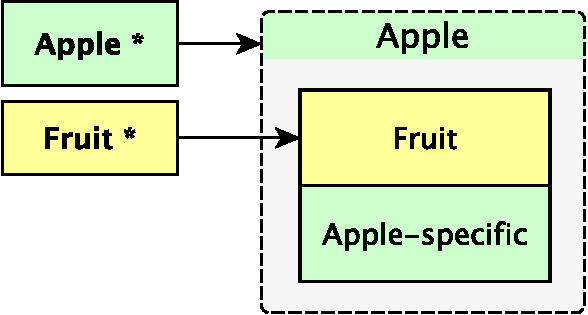
\includegraphics[width=0.6\textwidth]{illustrations/fruitptr-crop.pdf}
\caption{Преобразование указателя к базе}
\label{fig:fruitptr-crop}
\end{figure}

Мы использовали наследование в двух разных его ипостасях – унаследовав интерфейс базового класса и его код. В принципе наследование кода это почти всегда очень плохая идея. Старайтесь по мере возможности избегать наделять абстрактные классы состоянием и поведением. Для того, чтобы разработать хороший интерфейс фрукта, необходимо сделать его абстрактным, то есть оставить все методы без реализации, предоставив реализацию в производных классах. Давайте поговорим об этом подробнее.

\subsection{Полиморфизм}

При наследовании интерфейса \lstinline!get_mass!, наследовалась так же его реализация в общем предке. Но есть вещи, которые предок не знает как сделать за потомка. В этом случае логично предоставить потомку интерфейс, который во время выполнения вызовет нужный метод динамического типа. Простой и расхожий пример -- абстрактный класс фигуры совершенно точно не знает как рисуется ``фигура вообще'', зато это прекрасно знают его конкретные потомки -- квадрат, круг, овал -- каждый разумеется только о себе.

Рассмотрим как можно реализовать такой механизм без поддержки в языке, чтобы было понятно что делает для нас компилятор, обеспечивая нам поддержку. Изменим метод 

\lstinputlisting[firstline=14,lastline=24]{cpp_code/p2s7.cpp}

Разумеется в С++ нет необходимости ударяться в такой хардкор и язык предоставляет достаточно сахара чтобы спрятать под капотом практически все эти детали. Но пример поучителен. Во-первых для каждого метода, вызываемого через потомка необходимо иметь указатель на него (как \lstinline!m_entry! в примере выше). Вся совокупность таких указателей называется таблицей виртуальных методов. Важно понимать что таблица виртуальных методов это оверхед по памяти на каждый объект класса. Во-вторых, обратите внимание на то, что метод \lstinline!get_mass! очень прост и по сути сводится лишь к делегированию вызова по таблице виртуальных методов.

\subsubsection{Как подружить Дарта Вейдера\index{Dart Veider} с Пикачу\index{Pickachu}}\label{VirtualPolymorph}

Первое, что предоставляет язык С++ это возможность иметь в классе абстрактный, или чисто виртуальный метод, который обязан быть реализован по своему в каждом объекте (и компилятор проверит, что это действительно так). Таким образом мы как бы говорим компилятору что этот метод предназначен только для диспетчеризации вызова к методам произвольных классов. Второе -- это убранная под капот таблица виртуальных методов, от которой осталось только слово \lstinline!virtual! которое мы должны предпослать названию метода в базовом классе, не заботясь ни о заполнении элемента таблицы ни о конструкторе. Простой пример показывает мощь и гибкость этих средств.

\lstinputlisting[firstline=30,lastline=43]{cpp_code/p2s7.cpp}

Теперь можно писать довольно абстрактный код, полагающийся только на общий интерфейс объектов (способность сказать имя) и отдающий им на откуп детали реализации:

\lstinputlisting[firstline=45,lastline=59]{cpp_code/p2s7.cpp}

Это прекрасное свойство называется полиморфизм. Часто говорят, что полиморфизм является единственным оправданием для существования наследования, и что если в вашем классе нет ни одной виртуальной функции, наследование от него – дурной тон. 

\subsubsection{Статический и динамический тип\index{Dynamic type}}

Пока мы не стёрли с доски, ещё раз поглядим на функцию \lstinline!friendship!. Что можно сказать об аргументе \lstinline!n1!? Всего лишь, что его тип, объявленный в списке аргументов (иначе говоря статический тип) это константная ссылка на \lstinline!NamedObject!. Это всё, что компилятор может сказать об этом типе статически, без контекста исполнения.

Но динамически при вызове из \lstinline!main!, функция \lstinline!friendship! вызывается с двумя параметрами, один из которых имеет тип \lstinline!Pickachu!, другой – тип \lstinline!DartVeider!, оба являются производными классами от \lstinline!namedObject!, то есть, согласно принципу подстановки Лисков действительно могут быть использованы вместо него в любых контекстах.

То, что любая переменная может иметь разные статический и динамический типы в конкретной точке исполнения, это крайне важно, потому что при вызове виртуальной функции (как в примере выше) вызывается виртуальная функция, определённая в классе, соответствующем динамическому типу объекта, а при вызове невиртуальной функции – функция его статического типа.

Вызов функции статического типа также называется ранним или статическим связыванием, а вызов функции динамического типа называется поздним или динамическим связыванием (имеется в виду связывание функции с именем типа).

\subsubsection{Проблема срезки\index{Cutting}}\label{Cutting}

Мы всё ещё не стираем с доски и глядим на \lstinline!friendship!. Аргументы \lstinline!n1! и \lstinline!n2! переданы в неё по ссылке. В принципе, они могли бы быть переданы и по указателю:

\begin{lstlisting}
void friendship(const NamedObject *n1, const NamedObject *n2) /* still ok */
\end{lstlisting}

Но крайне дурным тоном является передача аргументов по значению.

\begin{lstlisting}
void friendship(const NamedObject n1, const NamedObject n2) /* error! */
\end{lstlisting}

Это происходит от того, что формальные аргументы конструируются при входе в функцию. Для указателей и ссылок всё нормально. Но попытка сконструировать объект абстрактного класса (то есть класса, содержащего хотя бы один чисто виртуальный метод) сама по себе ошибочна.

Хорошо, пусть даже это удалось. В этом случае новосконструированные объекты \lstinline!n1! и \lstinline!n2! уже не будут содержать частей от Дарта Вейдера и Пикачу, а станут безликими ``Именоваными объектами''. Этот срез информации при передаче по значению называется ``проблемой срезки''. Срезка часто возникает в практических контекстах и важно о ней помнить и избегать передавать параметры по значению.

\subsubsection{Параметры по умолчанию\index{default arguments} и виртуальные функции\index{virtual}}

Тонкий вопрос, который многие программисты на C++ часто упускают из виду это то, как ведут себя виртуальные функции с параметрами по умолчанию. Представим следующий код:

\lstinputlisting[firstline=1,lastline=21]{cpp_code/p2s7a.cpp}

Программист, читающий этот код, возможно, ожидает, что в этом случае будет нарисован зелёный прямоугольник. Но это не так. Прямоугольник будет нарисован красным цветом. Дело в том, что функции в C++ связываются динамически, а аргументы по умолчанию – статически. Таким образом для вызова draw компилятором будет сгенерирован вызов виртуальной функции с аргументом по умолчанию, объявленном в классе \lstinline!Shape!. Именно поэтому виртуальные функции с аргументами по умолчанию считаются крайне плохим тоном

\textbf{Домашняя наработка:} исследуйте самостоятельно поведение виртуальных функций с переменным числом аргументов.

\textbf{Домашняя наработка:} также самостоятельно исследуйте случай вызова виртуальной функции из конструктора или деструктора и чем это чревато.

\subsection{Перегрузка\index{overload} операторов\index{operator}}\label{OperatorOverloading}

Очень важным частным случаем полиморфизма в C++ и частой причиной ненависти разработчиков к чтению кода на этом языке является возможность перегружать для пользовательских типов такие операторы как ``+'', ``-'', ``*'' и т. п.

Рассмотрим классический пример – реализацию некоего пользовательского класса, оперирующего комплексными числами.

\lstinputlisting[firstline=8,lastline=20]{cpp_code/p2s8.cpp}

Благодаря такому определению, арифметику с комплексными выражениями можно записывать в форме, близкой к общепринятой.

\lstinputlisting[firstline=22,lastline=32]{cpp_code/p2s8.cpp}

Главная проблема здесь в том, что вы действительно вольны написать любой код в определении оператора сложения. Ваше сложение комплексных чисел не обязано удовлетворять даже каким-то базовым инвариантам сложения:

\begin{lstlisting}
assert (a + b == b + a); /* ORLY? */
\end{lstlisting}

Вместо этого ваша операция сложения может осуществлять вычитание, лезть в базу данных или форматировать диск. Почти всегда, когда вы читаете код на C++, вы обязаны иметь в виду, что не можете быть уверены что значит операция ``+'' этим утром. Ночью кто-нибудь мог вкоммитить в неё чудовищные изменения – из лучших побуждений, разумеется.

Всё усугубляется тем, что общий список операторов, которые можно переопределить, крайне внушающ. Его всегда можно посмотреть в стандарте, но кроме основных арифметических и логических операций, определение которых довольно таки прямолинейно, перегрузке могут подвергаться совершенно экзотические вещи – сравнение, присваивание, приведение к типу (любому, включая встроенные), обращение по указателю и даже выделение памяти с помощью new и её освобождение. Давайте побеседуем об нескольких специальных и проблематичных случаях переопределённых операторов.

\textbf{Домашняя наработка:} кстати а как бы вы определили оператор \lstinline!==! для комплексных чисел? Только помните, что определять сравнение чисел типа \lstinline!double! через \lstinline!==! это вообще не лучшая идея...

\subsubsection{Переопределение симметричных бинарных операций}\label{SymmBinary}

Для того, чтобы абстракция комплексных чисел была завершённой, должна быть возможность неявного преобразования double в complex, ведь по сути число \lstinline!2.0! это \lstinline!2.0 + 0.0 * i!. Эта возможность заложена в конструкторе класса (вспоминаем, что конструктор с одним аргументом это неявное преобразование типа).

\lstinputlisting[firstline=36,lastline=37]{cpp_code/p2s8.cpp}

Но здесь таится и опасность, потому что сложение перестаёт быть коммутативным и простая запись, вида:

\lstinputlisting[firstline=39,lastline=40]{cpp_code/p2s8.cpp}

Выдаст ошибку компиляции. Ошибка связана с тем, что неявные преобразования применяются только к параметрам, перечисленным в списке параметров. Поэтому \lstinline!a.operator+(2.0)! преобразует \lstinline!double! к \lstinline!Complex!, но для \lstinline!(2.0).operator+(a)! неявный параметр \lstinline!this! -- указатель на объект для которого вызывается метод, не подвергается, согласно стандарту, никаким неявным преобразованиям.

Правильный метод: определить операторы сложения и умножения вне класса как отдельные функции:

\lstinputlisting[firstline=8,lastline=29]{cpp_code/p2s8c.cpp}

Точно так же необходимо поступать со всеми функциями, которые по определению должны быть коммутативными. Тогда коммутативность будет сохранена.

\subsubsection{Переопределение выделения и освобождения памяти}

Переопределение \lstinline!new! и \lstinline!delete! в классах это всегда отдельная и крайне скользкая тема. Они уже были коротко рассмотрены выше, но теперь настало время уточнить подробности. Основным отличием \lstinline!new! от \lstinline!malloc! является то, что malloc выделяет просто кусок памяти, в то время как new конструирует объект -- в частности вызывает его конструктор, но не только. Например конструируется и заполняется таблица виртуальных методов. И опять-таки не только это. Во многом из-за всех этих ``не только'', детали которых следует пока оставить за кадром и может быть позже вернуться, напрямую вызвать конструктор в C++ нельзя, так что обойтись без new для этого не удастся. Но, использовав \lstinline!malloc()! для выделения буфера, вместе с так называемым размещающим new (placement new) можно обойтись без \lstinline!delete! (поскольку деструктор может быть явно вызван).

\lstinputlisting{cpp_code/p2s9.cpp}

В этом листинге наверное сейчас всё непонятно. Сделаем шаг назад и рассмотрим типичное выделение памяти:

\begin{lstlisting}
class Widget {};
...
Widget *w = new Widget;
\end{lstlisting}

Что здесь происходит? Неожиданно много всего.

\begin{enumerate}
\item
Сначала, по форме оператора new, компилятор определяет какой именно new имеется в виду. Существуют три нормальные формы new:
\begin{itemize}
\item
new в куче с возбуждением исключений при исчерпании памяти. Именно он использован в рассматриваемом примере.
\item
new в куче с возвратом нуля при исчерпании памяти
\item
размещающий new\index{placement new} (с размещением в заданном месте). Именно он и был использован в листинге выше. Его синтаксис похож на выделяющий new из этого примера, но буфер, в котором размещается сконструированный объект, не выделяется, а передаётся как параметр в скобках.
\end{itemize}

Кроме нормальных существуют ещё и специальные формы new, когда пользователь некоего типа переопределяет размещающий new этого типа передавая ему не область памяти, а нечто иное -- скажем область памяти и поток для записи лога и т.п. В следующем листинге показано использование разных форм new.

\begin{lstlisting}
class Widget {};
...
Widget *w = new Widget;
Widget *w = new (std::nothrow) Widget;
Widget *w = new (WidgetPool) Widget;
Widget *w = new (WidgetPool, WidgetLogStream) Widget;
\end{lstlisting}

Здесь первая строчка это \lstinline!malloc!+вызов контруктора с возбуждением исключения при ошибке выделения, вторая строчка это \lstinline!malloc!+вызов контруктора без возбуждения исключения при ошибки выделения (тогда в \lstinline!w! просто запишется \lstinline!NULL!), третья строчка это просто вызов конструктора на уже выделенную память (при этом неудачи выделения быть, разумеется, уже не может). И четвёртая строчка иллюстрирует специальную пользовательскую форму оператора \lstinline!new! и не будет у вас скомпилирована, без специальных объявлений внутри класса \lstinline!Widget!.

\item
Далее компилятор выделяет память в куче (строго при необходимости, размещающие и специальные формы пропускают этот пункт) и в случае нехватки памяти вызывает пользовательский обработчик, который можно поставить и на стандартное выделение с помощью \lstinline!set_new_handler!.
\item
Далее в случае если вызвана нормальная форма неразмещающего new, компилятор вызывает конструктор размещённого в куче объекта или все конструкторы, если был размещён массив.
\item
Разрушение происходит в обратном порядке.
\end{enumerate}

Давайте напишем класс для которого объявлены переопределения всех нормальных форм \lstinline!new!/\lstinline!delete! как это сделано в \cite{effcpp3d}.

\begin{lstlisting}
class StandardNewDeleteForms {
public:
static void *operator new(std::size_t size);
static void operator delete(void * memory);
static void *operator new(std::size_t size, const std::nothrow_t &nt);
static void *operator new(std::size_t size, void *ptr);
};
\end{lstlisting}

\textbf{Домашняя наработка:} 
Напишите и протестируйте код для каждого из переопределений.

C++ предоставляет достаточно тонкий инструментарий для работы с памятью, который необходимо использовать с осторожностью. Переопределяя каждый оператор не забывайте о возможном пользовательском вызове \lstinline!set_new_handler!. Переопределяя \lstinline!new! не забывайте переопределять соответсвующий \lstinline!delete!. Работайте с памятью осторожно и внимательно. И главное -- трижды подумайте нужно ли вам это вообще.

\subsubsection{Переопределение копирования и присваивания}

Представим пустой, сферический класс в вакууме.

\lstinputlisting[firstline=3,lastline=3]{cpp_code/p2s10.cpp}

Так ли он пуст, как это кажется на первый взгляд? Совершенно очевидно, что даже объект такого совершенно пустого класса в программе на C++ может быть создан, создан по образцу, скопирован и разрушен. Всю эту обвязку, если её не предоставляете вы, предоставляет компилятор C++. То есть написанное определение эквивалентно следующему:

\lstinputlisting[firstline=7,lastline=14]{cpp_code/p2s10.cpp}

Конструктор и деструктор должны быть к этому моменту уже понятны. Но мы видим, что C++ генерирует ещё две функции специального вида – копирующий конструктор\index{copy constructor}, отвечающий за создание объекта по образцу такого же и оператор присваивания\index{assignment operator}, который будет вызван при присваивании объекта в выражениях вида \lstinline!a=b!.

\lstinputlisting[firstline=20,lastline=22]{cpp_code/p2s10.cpp}

По умолчанию сгенерированные компилятором конструктор копирования и оператор присваивания просто побитово копируют код аргумента в целевой объект. Разумеется, это не пройдёт если в классе есть член-ссылка, тогда вы должны писать оператор присваивания самостоятельно.

\textbf{Домашняя наработка:} объяснить почему присваивание по умолчанию не годится при членах класса, являющихся ссылками.

Иногда такое умолчательное поведение приводит к мрачным проблемам, тяжёлым в отладке. Предположим, вы написали некий класс, управляющий внутренним буфером, который выделяется в конструкторе и освобождается в деструкторе.

\lstinputlisting[firstline=30,lastline=38]{cpp_code/p2s10.cpp}

А потом кто-то по незнанию скопировал его внутри какой-то функции.

\lstinputlisting[firstline=40,lastline=44]{cpp_code/p2s10.cpp}

Что при этом произойдёт? Выделенный вами буфер доступен по указателю. Указатель будет побитово скопирован. Это значит что теперь на буфер есть два указателя. При выходе за границы блока оба будут освобождены. Это крайне неприятная ошибка двойного освобождения и проблемы.

\begin{figure}[h!]
\centering
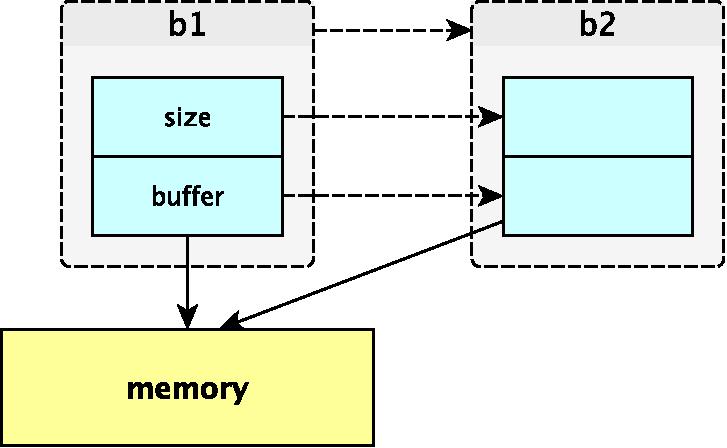
\includegraphics[width=0.6\textwidth]{illustrations/copying-crop.pdf}
\caption{Ошибка двойного освобождения}
\label{fig:copying-crop}
\end{figure}

Говорят, что по умолчанию C++ реализует поверхностное копирование (shallow copy\index{shallow copy}). Копирование с выделением нового буфера и копированием в него содержимого старого (ещё и с проверкой на присваивание самому себе) это глубокое копирование (deep copy\index{deep copy}) которое пользователь всегда должен реализовать самостоятельно.

\lstinputlisting[firstline=46,lastline=65]{cpp_code/p2s10.cpp}

Так всё будет работать. Но иногда копирование не нужно и его проще запретить, объявив собственные конструктор копирования и оператор присваивания в закрытой части класса.

\lstinputlisting[firstline=67,lastline=77]{cpp_code/p2s10.cpp}

Теперь компилятор не сгенерирует за вас неправильные варианты и копирование просто не будет скомпилировано.

\subsubsection{Оптимизации возвращаемого значения\index{RVO}}

RVO или оптимизация возвращаемого значения, прописана в стандарт C++ (например 12.3.2.15 для С++98) и она гласит, если коротко, что компилятор имеет право не вызывать копирующие конструкторы если он может статически доказать, что объекты эквивалентны.

Пример:

\begin{lstlisting}
#include <cstdio>

using namespace std;

class foo {
public:
  foo () { printf ("foo::foo()\n"); }
  foo (const foo&) { printf ("foo::foo( const foo& )\n"); }
  ~foo () { printf ("foo::~foo()\n"); }
};

foo
bar()
{
  foo local_foo;
  return local_foo;
}

int
main()
{
  foo f = bar();
  return 0;
}
\end{lstlisting}

В случае если GCC компилирует этот код без RVO (опция \lstinline!-fno-elide-constructors!), вывод на экран выглядит как:

\begin{lstlisting}
foo::foo()
foo::foo( const foo& )
foo::~foo()
foo::foo( const foo& )
foo::~foo()
foo::~foo()
\end{lstlisting}

Последовательность очевидна: создаётся локальный \lstinline!local_foo!, создаётся его копия -- возвращаемое значение, уничтожается \lstinline!local_foo!, возвращаемое значение копируется в \lstinline!f!, уничтожается возвращаемое значение, уничтожается \lstinline!f!.

В случае же обычной компиляции с RVO, вывод выглядит гораздо проще:

\begin{lstlisting}
foo::foo()
foo::~foo()
\end{lstlisting}

Эта экономия разрешена стандартом и поэтому программист не должен закладываться на то, что его конструктор копирования всегда будет вызван в контексте копирования.

\subsection{Динамическое приведение\index{dynamic\_cast} и RTTI\index{RTTI}}

Кроме всех операторов приведения, рассмотренных в предыдущей лекции, существует ещё один, разработаный специально, чтобы приводить статический тип к динамическому типу. Он называется \lstinline!dynamic_cast!. Его интересной особенностью является то, что он по-разному работает для указателей и для ссылок. Сначала разберём \lstinline!dynamic_cast! для указателей

\begin{lstlisting}
Derived* temp = dynamic_cast<Derived*>(base);
\end{lstlisting}

Пытается привести p, типа \lstinline!Base*! к типу \lstinline!Derived*!, где \lstinline!Base! и \lstinline!Derived! принадлежат одной и той же иерархии. Если \lstinline!Derived! является базовым классом для \lstinline!Base!, то это ничем не отличается от \lstinline!static_cast!. Но \lstinline!dynamic_cast! работает также если Base является полиморфным базовым классом для \lstinline!Derived!, то есть является базовым классом для \lstinline!Derived! и содержит виртуальные функции. Звучит запутано? Давайте посмотрим пример.

\lstinputlisting{cpp_code/p2s13.cpp}

Что будет на выдаче? Ответ:

\begin{lstlisting}[language=make]
You are Dart Veider!
You are not Dart Veider, you are Pokemon
\end{lstlisting}

Коротко говоря, \lstinline!dynamic_cast!, использованый для указателя даёт возможность ``спросить'' такой ли у этой переменной динамический тип, как он полагает. Он приводит к этому типу если ответ ``да'' или возвращает \lstinline!NULL!, если ответ ``нет''.

При использовании \lstinline!dynamic_cast! для ссылок, вопрос превращается в утверждение. Если это утверждение нарушается, кидается исключение, но о них мы поговорим в другой раз.

Для \lstinline!dynamic_cast! очень важно, чтобы в базовом классе была хотя бы одна виртуальная функция. Очень часто отличным кандидатом на роль такой функции является виртуальный деструктор, о котором мы сейчас поговорим.

\subsection{Виртуальные деструкторы}\label{virtdestr}

Для программиста на C++ важно знать один очень специальный случай полиморфизма, относящийся к семантике освобождения, а именно виртуальные деструкторы. Рассмотрим пример – пусть у нас есть некий класс измерителя времени и фабричная функция, которая в зависимости от точности, с которой пользователю необходимо измерять время, возвращает ему какие-нибудь часы от солнечных до атомных.

\lstinputlisting{cpp_code/p2s14.cpp}

Что произойдёт при уничтожении, если деструктор будет не виртуальным? Будет освобождена базовая часть, но не будет освобождена производная часть, что неминуемо приведёт к утечкам памяти и проблемам. Если же сделать деструктор виртуальным, то будет автоматически правильно вызван деструктор производного класса по указателю на базовый.

Наличие в классе невиртуального деструктора является в мире промышленного программирования достаточным основанием никогда ничего не наследовать от этого класса. Обратное – плохой тон. 

\subsection{Проблемы, возникающие при проектировании открытого наследования}

Принцип подстановки Лисков требует навыка при работе с ним. Предположим, вы проектируете иерархию геометрических объектов и столкнулись с необходимостью расположить в ней такие абстракции как ``квадрат'' и ``прямоугольник''. Первой мыслью может быть унаследовать прямоугольник от квадрата – в конце концов прямоугольник вводит ещё одно поле и может быть какие-нибудь дополнительные методы

\lstinputlisting[firstline=3,lastline=20]{cpp_code/p2s11.cpp}

Но такой подход создаёт проблемы, связанные с тем, что прямоугольник не является частным случаем квадрата и здесь нарушается принцип подстановки. 

Вопрос к студентам: опишите проблемы которые может вызвать такое проектирование. Например рассмотрите реализованную в \lstinline!Square! (и даже виртуальную) функцию \lstinline!void increase(int times)!, в times раз увеличивающую площадь квадрата. Как вы реализуете её для прямоугольника?

\textbf{Домашняя наработка:} рассмотрите вариант наследования квадрата от прямоугольника. К чему это приводит?

Подсказка: совсем ничего хорошего, как вы догадываетесь.

\subsection{Иерархии}

Продолжим разговор о наследовании. До сих пор рассматривалось только одиночное одноуровневое наследование, но C++ даёт в этом отношении гораздо больше свободы. Один класс может наследовать многим классам, которые сами кому-то наследуют и так далее. Для этого базовые классы с их модификаторами доступа перечисляются через запятую

\begin{lstlisting}
class Man: public AnimalsWithTwoLegs, public OnesWithoutWings {};
\end{lstlisting}

Это позволяет строить иерархии взаимодействующих классов и объектов при проектировании сложных программных систем.

\begin{figure}[h!]
\centering
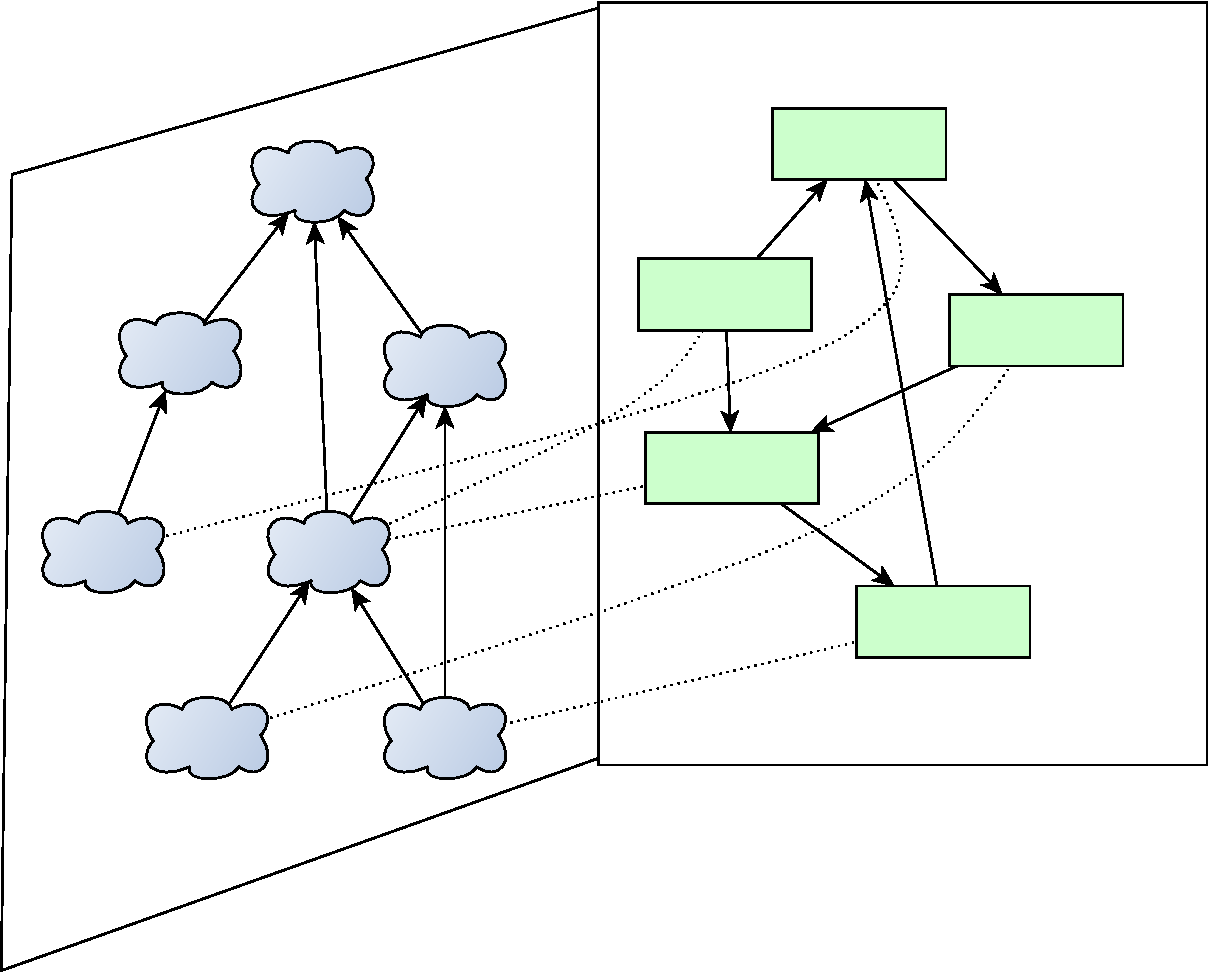
\includegraphics[width=0.8\textwidth]{illustrations/hierarchies-crop.pdf}
\caption{Иерархии классов и объектов}
\label{fig:hierarchies-crop}
\end{figure}

Проектирование хорошей иерархии это всегда сложный инженерный процесс, выходящий за рамки этого курса. Зато можно на игрушечных примерах рассмотреть основные проблемы, ожидающие разработчика на этом пути.

\subsubsection{Ромбовидные схемы и виртуальные базовые классы}

Предположим, вы проектируете систему, поддерживающую абстракции файлов ввода и вывода. Рано или поздно вы пришли к чему-то вроде такого

\begin{lstlisting}
class File {};
class InputFile : public File {};
class OutputFile : public File {};
class IOFile : public InputFile, public OutputFile {};
\end{lstlisting}

Графически это может быть выражено ромбовидной схемой

\begin{figure}[h!]
\centering
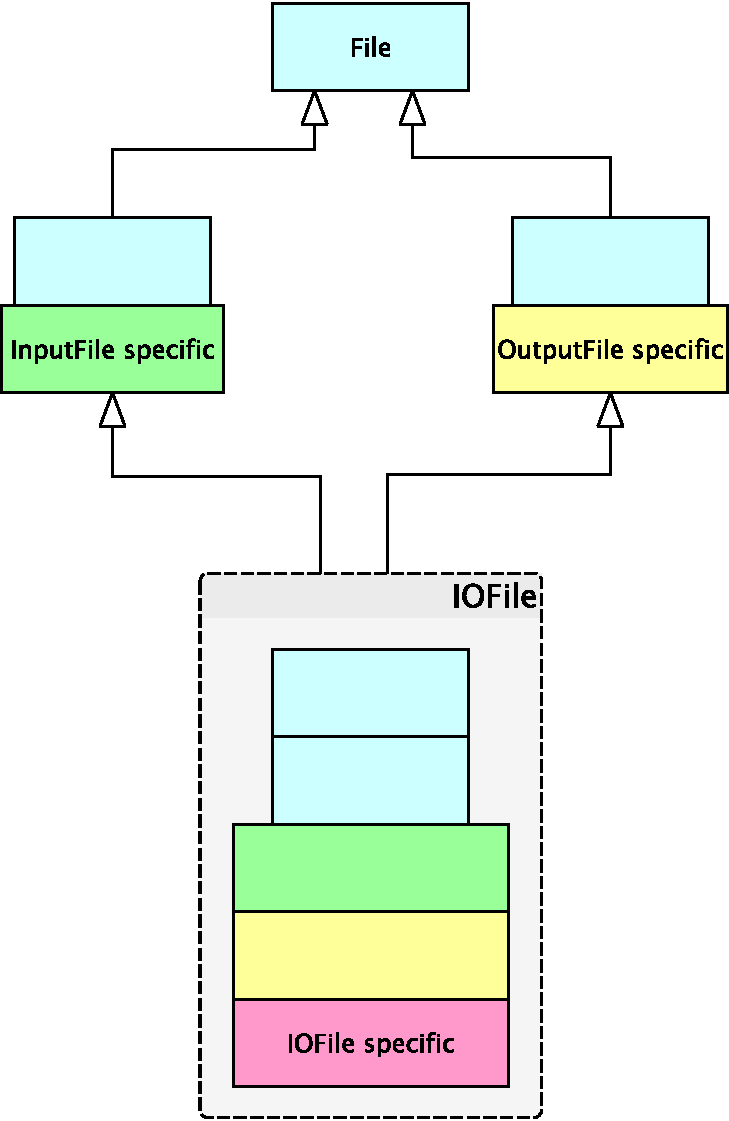
\includegraphics[width=0.5\textwidth]{illustrations/romb-crop.pdf}
\caption{Ромбовидная схема}
\label{fig:romb-crop}
\end{figure}

Предположим, что в классе \lstinline!File! есть поле \lstinline!File::filename!. По умолчанию, в классе \lstinline!IOFile! у вас получится два члена: \lstinline!InputFile::File::filename! и \lstinline!OutputFile::File::filename!, но файл у которого два имени это абсурд. Чтобы избежать такой ситуации, базовый класс в наследовании может быть объявлен виртуальным (ещё можно вообще никогда ничего не писать на C++, а использовать C, это предпочтительный вариант).

\begin{lstlisting}
class File {};
class InputFile : virtual public File {};
class OutputFile : virtual public File {};
class IOFile : public InputFile, public OutputFile {};
\end{lstlisting}

Теперь всё хорошо и в ромбовидной схеме у самого нижнего производного класса есть только одна копия базового.

\subsubsection{Порядок инициализации в сложных диаграммах}

Важно очень хорошо представлять себе порядок конструирования сложных диаграмм классов. Представим несколько синтетический (но на самом деле гораздо менее сложный, чем многие практически важные иерархии) пример.

\lstinputlisting[firstline=3,lastline=15]{cpp_code/p2s12.cpp}

Для простоты можно изобразить эту иерархию на листочке:

\begin{figure}[h!]
\centering
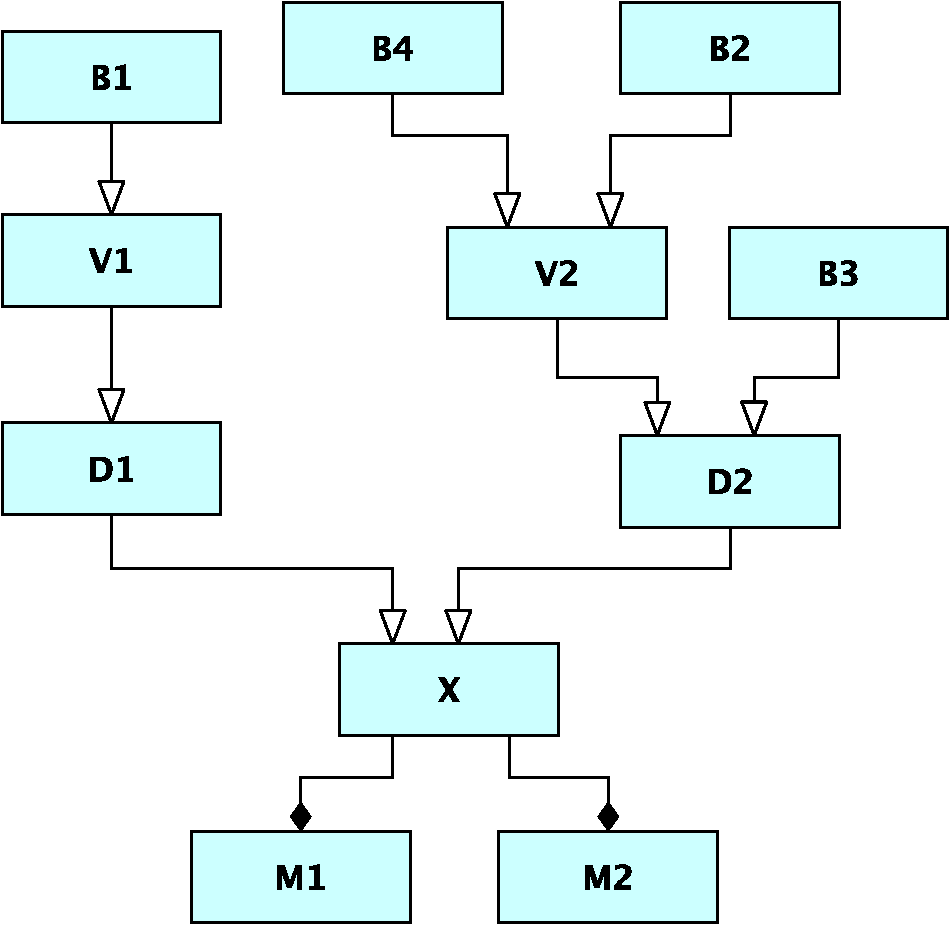
\includegraphics[width=0.5\textwidth]{illustrations/complexhier-crop.pdf}
\caption{Сложная иерархия}
\label{fig:complexhier-crop}
\end{figure}

Порядок инициализации объекта класса \lstinline!X! для изображённой иерархии следующий:

\begin{itemize}
\item Сначала конструируются виртуальные базовые классы
  \begin{enumerate}
  \item Конструирование \lstinline!V1!: \lstinline!B1::B1()!, \lstinline!V1::V1()!
  \item Конструирование \lstinline!V2!: \lstinline!B1::B1()!, \lstinline!B2::B2()!, \lstinline!V2::V2()!
  \end{enumerate}
\item Затем конструируются невиртуальные базовые классы
  \begin{enumerate}
  \item Конструирование \lstinline!D1!: \lstinline!D1::D1()!
  \item Конструирование \lstinline!D2!: \lstinline!B3::B3()!, \lstinline!D2::D2()!
  \end{enumerate}
\item Затем конструируются члены \lstinline!M1::M1()!, \lstinline!M2::M2()!
\item И в последнюю очередь выполняется конструктор \lstinline!X::X()!
\end{itemize}

Вид наследования (открытое, закрытое или защищённое) не влияет на порядок инициализации.

\subsubsection{Вложенные классы и снова о пространствах имён}

Вложенные функции в C++ невозможны так же как и в C (что кстати не вполне логично, так как вложенные лямбда-функции в новом стандарте возможны и будут рассмотрены на следующих лекциях, так что казалось бы гулять так гулять). Зато C++ позволяет вкладывать классы. Синтаксис очевиден, но, если необходимо, чтобы вложенный класс ``знал'' о своём окружении, об этом надо позаботиться отдельно:

\lstinputlisting{cpp_code/p2s15.cpp}

Каждый вложенный класс определяет область видимости своих имён. Таким образом, можно создать отдельный объект типа \lstinline!DeathStar::DartVeider!, но можно и запретить это, поместив его в private. Собственно обычные пространства имён имеют всего одно отличие от классов со всеми открытыми статическими членами. В случае обычных пространств имён вы можете писать много их объявлений и все они будут объединены компилятором. Таким образом, даже зная как можно сэмулировать их классами, есть смысл всё же использовать пространства имён.

\subsection{Скажи мне кто твой друг}

Модель инкапсуляции C++ логична и стройна (общий смех). В общем случае закрытые члены класса формируют его состояние и недоступны извне, иначе, чем через его методы, отражающие поведение -- это хорошо и правильно. Но в некоторых случаях, разработчик хотел бы дать некоему классу эксклюзивный доступ к закрытым членам другого класса. Например для того, чтобы не писать кучу геттеров и в то же время сохранить консистентность абстракции. Для этого язык C++ предусматривает механизм друзей (\lstinline!friend!) класса.

\lstinputlisting[firstline=8,lastline=16]{cpp_code/p2s16.cpp}

Класс \lstinline!Node!, назначив себе друга \lstinline!BinaryTree!, открыл ему всё свое закрытое состояние, но, при этом, сам не получил никакого доступа к \lstinline!BinaryTree!. Теперь внутри BinaryTree можно написать код вида:

\lstinputlisting[firstline=32,lastline=49]{cpp_code/p2s16.cpp}

Класс может открывать своё состояние не только классам, но и функциям. Скажем, не открывая доступ всему \lstinline!BinaryTree!, можно открыть его только методу \lstinline!find!:

\lstinputlisting[firstline=20,lastline=28]{cpp_code/p2s16.cpp}

Дружба не наследуется, но друг статического родительского типа достаточен, чтобы делать дружественные вызовы полиморфных наследников.

\lstinputlisting[firstline=51,lastline=80]{cpp_code/p2s16.cpp}

В общем случае, дружба статических типов вредна для инкапсуляции. Но дружба, позволяющая полиморфные вызовы по большой и закрытой иерархии это полезно и иногда необходимо. Также, дружба может быть полезна во многих неожиданных контекстах при работе с шаблонами, которые будут рассмотрены ниже.

\subsection{Мелкие детали, касающиеся объектной модели C++}

\begin{enumerate}
\item
Указатель на статическую функцию-член ничем не отличается от указателя на функцию
\item
Указатель на нестатическую функцию-член \lstinline!int (Complex::*)(double,double)! содержит имя класса, содержащего данный метод
\item
Вызов функции-члена объекта \lstinline!complnum! через указатель на функцию-член \lstinline!p! выглядит как \lstinline!(complnum.*p)(1.0, 3.14);!
\end{enumerate}

\pagebreak
\subsection{Домашняя наработка по части 3}

\begin{enumerate}
\item
Расширьте приведённый в (\ref{BallGame}) код до трёхмерной игры в мяч

\item
Введите в приведённый в (\ref{BallGame}) код примитивы синхронизации чтобы его можно было запускать в многопоточном окружении

\item
Расширьте приведённый в (\ref{BallGame}) код до игры в мяч со смещающимся центром тяжести (допустим мяч наполовину заполнен водой или песком)

\item
Разработайте конкретный класс \lstinline!CTime!, предназначенный для хранения текущего времени и вычисления временных интервалов. Не ограничивайтесь unix time, сделайте возможным, например, подсчёт количества часов от Куликовской битвы до Бородинского сражения

\item
Как можно улучшить рассмотренный в (\ref{RAII}) класс CFile? Реализуйте и протестируйте обёртку.

\item
Разработайте и реализуйте иерархию классов, для управления сетевым соединением. Предусмотрите как минимум классы для TCP и UDP сокетов, наследующие от общего предка

\item
Реализуйте абстрактный интерфейс материальной точки и унаследуйте от него разные варианты мяча -- идеальный, с сопротивлением воздуха, со смещённым центром тяжести, etc. На основе общего интерфейса, реализуйте игрока в мяч, которому всё равно каким мячом играть

\item
Перегрузите для класса комплексных чисел, приведённых в (\ref{OperatorOverloading}) инкремент, логические операции, вычитание

\item
Разработайте класс кватернионов со всеми перегруженными арифметическими операциями. Исследуйте есть ли смысл наследовать его от комплексных чисел.

\item
Разработайте класс для операций над матрицами. Проиллюстрируйте к каким проблемам может привести ставшее некоммутативным умножение.

\item
Для вашего класса операций над матрицами перегрузите выделение и освобождение памяти. Разработайте стратегию выделения памяти для разреженных матриц. Проиллюстрируйте умножение двух разреженных матриц 10000x10000 в каждой из которых значимыми являются всего 2-3 элемента (остальные нули).

\end{enumerate}

\pagebreak
\section{Особая шаблонная магия}

Шаблоны, введённые в C++ были в своё время введены туда экспериментально. Их не было ни в одном другом языке и никто по настоящему не знал, что из этого получится. Поэтому большинство интересных и важных свойств шаблонов не были разработаны. Они были открыты. На этой лекции нас тоже ожидают открытия.

\subsection{Шаблоны функций\index{function template}}

Ранее, в разделе (\ref{ConstVsDef}) уже приводился пример преимущества C++ в объявлении обобщённых функций без использования макросов. Теперь самое время снова на него посмотреть и постараться достичь понимания сути происходящего.

\lstinputlisting[firstline=5,lastline=9]{cpp_code/p3s01.cpp}

Говорят, что здесь объявлен шаблон функции. Синтаксис шаблона ясен из определения: после слова \lstinline!template! в треугольных скобках через запятую перечисляются параметры шаблона. Подробности грамматики изложены в разделе 14 стандарта C++ \cite{stdcpp98}.

\begin{lstlisting}
template <typename T, class U, int x>
\end{lstlisting}

Здесь слово \lstinline!typename! означает параметр шаблона, задающий имя типа. По историческим причинам можно использовать \lstinline!class!, но новый стандарт поощряет использование \lstinline!typename!. Кроме того вы уже должны видеть в функции \lstinline!max()! существенный недостаток – параметры, передающиеся по значению, в случае увесистого \lstinline!T! будут неэффективны, лучше заменить их константными ссылками.

В расширенном и исправленном примере, заодно можно посмотреть как именно шаблоны функций ведут себя при перегрузке.

\lstinputlisting{cpp_code/p3s1.cpp}

Все эти правила довольно сложно выучить поэтому нужно просто осознавать что они есть и найти место в стандарте, откуда их можно вывести. Кроме того, полезно много экспериментировать, это создаёт ни с чем не сравнимое ``чувство'' языка, его возможностей и ограничений.

\textbf{Домашняя наработка:} рассмотрите случай, когда одновременно объявлены одновременно шаблоны для ссылки и константной ссылки

\begin{lstlisting}
template <typename T> inline T& max (T& a, T& b) { /* ... */ }
template <typename T> inline T const& max (T const& a, T const& b) { /* ... */ }
\end{lstlisting}

Как в этом случае будет разрешаться перегрузка? Приведите примеры. Аналогично для указателя, константного указателя, указателя на константные данные. Если добавить к перегрузке по ссылке перегрузку по значению, создав тем самым неоднозначность, компилятор должен отреагировать ошибкой. Проверьте как отработает эту ситуацию ваш компилятор.

\subsubsection{Когда C++ быстрее, чем C}\label{CppBetterC}

Простые шаблоны функций не так просты и их не стоит недооценивать. Вопрос к студентам: какую сигнатуру вы напишете, если хотите на C написать обобщённую функцию сортировки? Стандарт языка C99 регламентирует (пункт 7.20.5.2) следующую сигнатуру:

\begin{lstlisting}
void qsort(void *base, size_t nmemb, size_t size, int (*compar)(const void *, const void *));
\end{lstlisting}

Почему здесь использован \lstinline!void*!? Потому что в обобщённой функции мы не знаем какого типа элементы будут отсортированы. Кроме того требуется передавать размер элемента и их количество раздельно, что открывает возможности для человеческих ошибок. Но хуже всего то, что компаратор (вызываемый на каждое сравнение элементов) это указатель на функцию. Из-за этого:

\begin{itemize}
\item Каждый вызов компаратора имеет штраф на разыменование указателя на функцию -- лишний уровень косвенности
\item Исключена возможность inline-подстановки сравнения, которое обычно сводится к чему-то очень простому (скажем простому ``меньше, чем'')
\end{itemize}

Всех этих недостатков лишена реализация в стиле C++, которая может выглядеть примерно как:

\begin{lstlisting}
/* we suppose that Element class have meaningfull operator< () redefinition */
template <typename Element>
void qsortpp(Element *base, size_t nmemb);
\end{lstlisting}

Это лучше, проще, более безопасно относительно типов и это гораздо эффективнее. Платим мы за это объёмом кода, который компилятор теперь сгенерирует для каждой инстанциации \lstinline!qsort!, но это недорого.

На самом деле стандарт C++98 регламентирует (пункт 25.3.1.1) даже более изящную сигнатуру для стандартной сортировки:

\begin{lstlisting}
template<class RandomAccessIterator>
void sort(RandomAccessIterator first, RandomAccessIterator last);
\end{lstlisting}

Но вся её мощь, красота и обобщённость проявятся позже, когда речь пойдёт о стандартной библиотеке.

\textbf{Домашняя наработка:} Реализуйте \lstinline!qsort! в стиле C и в стиле C++

\subsection{Простые шаблоны классов\index{class template}}

Представьте, что перед вами стоит задача спроектировать стек – класс объектов любого типа (но однородных) которые будут туда помещаться и вытаскиваться. Как обычно синтаксис вполне понятен через пример (детали вы всегда сможете прочитать в стандарте).

\lstinputlisting[firstline=6,lastline=18]{cpp_code/p3s2.cpp}

Обратите внимание на то, что \lstinline!T!, помещённый в шаблон, используется внутри класса как совершенно обычный тип. Можно вернуть его из метода, передать в метод и даже использовать как деталь реализации скрытой подструктуры.

\lstinputlisting[firstline=20,lastline=37]{cpp_code/p3s2.cpp}

Вопрос к студентам: что мы забыли?

Ожидается хоровой ответ: деструктор, копирующий конструктор и оператор присваивания. Позвать кого-нибудь к доске разобрать как их писать.

Давайте посмотрим как применять разработанный шаблонный класс:

\lstinputlisting[firstline=39]{cpp_code/p3s2.cpp}

Из примера ясно, что с использованием шаблонов, поддержка двух разнородных контейнеров (трёх, десяти) это крайне легко. Скорость компиляции, правда, страдает, вместе с объёмом кода, но по современным реалиям это невысокая цена.

\subsubsection{Специализация\index{template specialization}}

В случае с функциями был использован механизм перегрузки функций чтобы получить специальное поведение для конкретного типа аргументов. Но нельзя ``перегрузить'' класс. Зато вы можете специализировать шаблон класса для конкретных шаблонных параметров. Синтаксис, опять же, прост:

\begin{lstlisting}
template <>
class Stack<int> { ... };
\end{lstlisting}

Такая запись создаёт отдельное поведение для стеков, инстанцированных целыми числами. Реализация и поведение такого шаблона могут не иметь вообще ничего общего с исходным. Это создаёт почти такую же радость при чтении кода на C++ как перегрузка операторов и неявные приведения.

\subsubsection{Частичная специализация\index{partial specialization}}

Суть частичной специализации в том, что вы пишете отдельный код для определённых обстоятельств инстанциирования, но часть параметров этого кода всё ещё задаёт шаблон. При исходном шаблоне

\begin{lstlisting}
template <typename T, typename U> class MyClass { ... };
\end{lstlisting}

Мы можем написать например такие специализации

\begin{lstlisting}
/* partial specialization: both template parameters have same type */ 
template <typename T> class MyClass<T,T> { ... }; 
/* partial specialization: second type is int template <typename T> */ 
class MyClass<T,int> { ... }; 
/* partial specialization: both template parameters are pointer types */
template <typename T1, typename T2> class MyClass<T1*,T2*> { ... };
\end{lstlisting}

И далее посмотрим как конкретные объявления будут раскрыты.

\begin{lstlisting}
MyClass<int,float> mif;    /* uses MyClass<T1,T2> */ 
MyClass<float,float> mff;  /* uses MyClass<T,T> */ 
MyClass<float,int> mfi;    /* uses MyClass<T,int> */ 
MyClass<int*,float*> mp;   /* uses MyClass<T1*,T2*> */
\end{lstlisting}

Учтите, что если под некое объявление подходят сразу два варианта частичной специализации, то это ошибка

\begin{lstlisting}
MyClass<int,int> m;        // ERROR: matches MyClass<T,T> 
                           //        and MyClass<T,int> 
MyClass<int*,int*> m;      // ERROR: matches MyClass<T,T> 
                           //        and MyClass<T1*,T2*>
\end{lstlisting}

Можно исправить ошибку сделав уникально подходящий шаблон

\begin{lstlisting}
template <typename T> 
class MyClass<T*,T*> { ... };
\end{lstlisting}

Правила частичной специализации также необходимо усвоить путём внимательного чтения стандарта и применять уместно.

\subsubsection{Разное о параметрах шаблонов}

Параметры шаблонов могут идти по умолчанию, в этом они похожи на параметры по умолчанию функций. Точно так же как параметры функций по умолчанию, параметры шаблонов по умолчанию связываются статически.

\begin{lstlisting}
template <typename T, typename U = int> class MyClass { ... };
MyClass<int> foo; /* MyClass <int, int> */
\end{lstlisting}

Применять их следует с осторожностью.

Очень часто возникает идея параметризовать некий шаблон неким шаблоном. Рассмотрим простой пример инстанцирования стека стеков, чтобы понять синтаксис:

\begin{lstlisting}
Stack < Stack<int> > stack;
\end{lstlisting}

Вложение таким образом можно осуществлять теоретически бесконечно. Реально больше трёх уровней уже крайне плохой тон (и чревато комбинаторными взрывами).

\subsection{Шаблоны членов и инкапсуляция}

До сих пор шаблоны классов и шаблоны функций рассматривались раздельно, но в принципе шаблонная функция тоже может быть членом класса. Это не вносит почти никаких изменений в рассмотренный материал -- для неё верно всё то же, что и для других шаблонных функций. Но использование шаблонных членов вносит серьёзные коррективы в инкапсуляцию. Коротко говоря, использование шаблонных членов отменяет инкапсуляцию. Рассмотрим класс:

\begin{lstlisting}
class X {
public:
  X() : private_(1) {}
  tempalte <typename T> void f(const T& t) { /* ... */ }
  int Value(void) const { return private_; }
private:
  int private_;  
};
\end{lstlisting}

За счёт наличия в этом классе шаблонного члена, человек, использующий его, может написать код:

\begin{lstlisting}
namespace {
  struct Y {};
}
template<>
void X::f(const Y&) {
  private_ = 2;
}
\end{lstlisting}

Этот код эксплуатирует оговорённую в стандарте возможность специализировать шаблон-член для любого типа. Это выглядит забавно -- специализацию шаблонов-функций заменяет перегрузка, но шаблон-член вы можете как перегрузить, так и специализировать. Эта ортогональность прекрасна, если ей не злоупотреблять.

То, что шаблоны-члены неявно нарушают инкапсуляцию -- последствие взаимодействия объектно-ориентированной и шаблонной подсистем языка, которые проектировались во многом ортогонально и имеют нюансы совместного использования. Ещё о некоторых нюансах пойдёт речь далее, но прежде мы остановимся на альтернативах объектно-ориентированной модели, которые предлагаю шаблоны. И главная из них это шаблонный полиморфизм как альтернатива ОО-полиморфизму.

\subsection{Два полиморфизма\index{Template Polymorphism}}

Что же, к этому моменту вы знаете о шаблонах уже достаточно, чтобы вернуться к серьёзным вещам, таким как Дарт Вейдер и покемоны. Идея наследовать их от общего предка, как мы это делали в (\ref{VirtualPolymorph}), действительно хороша, если вы программист на Java, где вообще всё наследуется от общего предка. Но на C++ вы можете написать два отдельных класса:

\lstinputlisting[firstline=5,lastline=13]{cpp_code/p3s3.cpp}

И тем не менее сохранить возможность писать довольно абстрактный код, полагающийся только на общий интерфейс объектов (способность сказать имя) и отдающий им на откуп детали реализации:

\lstinputlisting[firstline=15,lastline=29]{cpp_code/p3s3.cpp}

Это прекрасное свойство называется полиморфизм времени компиляции, или статический полиморфизм. Заметьте, никаких больше виртуальных функций, никаких таблиц виртуальных методов, никакого оверхеда времени выполнения (за счёт раздутия кода помещением туда 100500 экземпляров функции \lstinline!friendship!, разумеется).

Разница в том, что класс \lstinline!NamedObject! создавал нам явный интерфейс, в случае же статического полиморфизма, шаблонная функция накладывает неявные требования к обоим своим инстанциирующим типам, сформулированное точно так же ``поддерживать функцию-член \lstinline!whoareyou(void)!''. 

При рассмотрении нового стандарта, будут рассмотрены ``концепты'', которые наконец-то определяют способ задать неявный интерфейс явно.

\subsubsection{Когда шаблонный полиморфизм уступает динамическому}

Использование шаблонного полиморфизма снижает накладные расходы на исполнение и почти всегда предпочтительно. Но есть вещи, которые требуют динамического полиморфизма и оказываются неоправданно сложными если пытаться сделать их на этапе компиляции.

\begin{lstlisting}
class obj
{
public:
  virtual int foo (int) = 0;    
};

class A : public obj;
class B : public obj;

/* ... class C, D, etc ... */

/* returns A is config have 'a', B is 'b', and so on ... */
obj * getfromconfig (const char *filename);

int
entry (obj *x)
{
  return x->foo();
}

int
main (void)
{
  return entry (getfromconfig("my.xml"))
}
\end{lstlisting}

Этот код представляет собой идиому ``виртуального конструктора'' (так же известен как фабричный метод).

\textbf{Домашняя наработка:} попробуйте переписать его с использованием только статического полиморфизма.

\subsection{Ваш друг typename\index{typename}}

Это ваш второй воображаемый друг, первый был, как вы помните, \lstinline!typedef!. Изначально \lstinline!typename! был введен в C++ чтобы явно указывать компилятору на вложенные шаблонные типы. Рассмотрим код:

\begin{lstlisting}
template <typename T>
int foo (const T& x)
{
  T::subtype *y;
  /* ... */
}
\end{lstlisting}

Что здесь написано? Думаете объявление указателя на вложенный тип? Вы не поверите, но дословно здесь написано 
следующее: ``В классе \lstinline!T! должен быть статический член с именем \lstinline!T::subtype!. Необходимо \textbf{умножить} его на некую (очевидно глобальную) переменную \lstinline!y! и проигнорировать результат''. Печально, да? Давайте исправим код:

\begin{lstlisting}
template <typename T>
int foo (const T& x)
{
  typename T::subtype *y;
  /* ... */
}
\end{lstlisting}

Теперь всё хорошо, мы явно указали компилятору, что \lstinline!T::subtype! это тип. Именно так \lstinline!typename! и был запланирован. По английски устранение такой неоднозначности называется ``\textbf{disambiguation}'' \index{disambiguation} и именно так этот термин устоялся в англоязычной литературе (не встречал его в русскоязычной). То, что я перевожу disambiguation как ``устранение неоднозначности'' это некая вольность, скорее передающая смысл термина, чем его перевод.

В использовании \lstinline!typename! для вложенных шаблонных классов может встретится один небольшой трюк -- дополнительное использование слова \lstinline!template! для устранения неоднозначности при разборе шаблона. Представим у нас есть код:

\lstinputlisting[firstline=5,lastline=18]{cpp_code/p3s4.cpp}

И надо написать вызов для шаблонной функции вложенного класса (например из другого шаблонного класса, с достаточно простым определением)

\begin{lstlisting}
template <typename T1, typename T2>
class Usage
{
public:
  void caller( /* parameter type */ &obj )
    {
      /* obj.nested<int>(); */
    }
};
\end{lstlisting}

Можно написать простую проверочную программу, где использовать этот вызов как-то так:

\lstinputlisting[firstline=31]{cpp_code/p3s4.cpp}

Сам по себе этот пример представляет собой лишь изящную головоломку, но полезен для иллюстрации концепции. В реальных проектах эти проблемы могут всплыть в гораздо более сложном коде и нужно вдоволь натренироваться на простых примерах, чтобы уметь их угадывать. Правильный ответ выглядит несколько необычно:

\lstinputlisting[firstline=20,lastline=28]{cpp_code/p3s4.cpp}

Но что произойдёт если мы не упомянем ключевого слова \lstinline!template!? Примерно та же проблема, что и с \lstinline!typename! -- компилятор не будет в точности знать как ему трактовать треугольную скобку, открывающуюся после имени типа \lstinline!Inner! или после имени функции \lstinline!nested!. И в том и в другом случае, без явного указания ключевого слова template, он будет трактовать эту скобку как переопределённый оператор ``меньше'' (снова нечто невероятное). Это может привести вас к массе неявных но интересных ошибок.

\subsection{Наследование от шаблона и CRTP\index{CRTP}}

Шаблонный класс со всеми определёнными парамтерами это уже настоящий класс и значит от него можно наследоваться. На этой технике основана интересная и часто используемая идиома CRTP.

\textbf{CRTP – curiously reccuring template parameter} означает параметризацию шаблона, являющегося базовым классом, шаблонным параметром, являющимся самим классом-потомком. Предположим, вы проектируете класс, реализующий абстракцию лазерного меча. При попытке ударить лазерным мечом, он должен попросить своего владельца использовать Силу. Тогда ваш код может выглядеть как-то так:

\lstinputlisting{cpp_code/p3s5.cpp}

По сути, здесь CRTP это способ для класса DartVeider попросить себе лазерный меч, который понимает, что он лазерный меч Дарта Вейдера. Подобным образом стек может попросить себе аллокатор, который понимает что он аллокатор для стека и т.п.

Вы должны хорошо освоиться с этой идиомой, она нам пригодится при разговоре про STL.

\subsection{Правила инстанцирования и SFINAE\index{SFINAE}}

Выше уже несколько раз было употреблено слово ``инстанцирование''. Интуитивно оно понятно, но оно имеет разный смысл для обычных классов (там инстанцирование класса это создание его объекта) и для шаблонов. Настало время дать этому слову более точное определение.

\textbf{Шаблонным инстанцированием} называется процесс порождения типов и функций из обобщённых шаблонных определений.

В книгах по шаблонам, таких как \cite{vandervoord} традиционно много места отводится тому, что называется ``Separation model''\index{Separation model}. Это модель инстанцирования, когда код шаблона находится в одной единице трансляции, а инстанцирование происходит в другой. Начиная с C++11 \cite{stdcpp11} экспорт шаблонов был запрещён, а Separation model объявлена устаревшей. Поэтому мы далее будем полагать, что код шаблона и инстанцирование происходят в одной единице трансляции.

Самое важное, что нужно знать про инстанцирование -- оно по стандарту обязано работать лениво. Это означает, что проверены на корректность будут только те части шаблона, которые действительно были использованы. Давайте рассмотрим пример:

\lstinputlisting{cpp_code/p3s6.cpp}

Несмотря на то, что инстанцирование определяет \lstinline!typedef! с некорректным параметром размера массива, это не является ошибкой, поскольку реально этот зависимый тип нигде не был использован. Ленивость вынуждает компилятор откладывать инстанцирование любой части шаблона так долго, как это возможно.

Ещё более разрешающей идиомой в правилах инстанцирования является SFINAE, что означает \textbf{substitution failure is not an error}. Она означает, что некорректная подстановка шаблонных параметров сама по себе не является ошибкой. SFINAE является очень мощной техникой, позволяющей делать интересные вещи. Например определить на этапе компиляции имеет ли некий тип вложенный зависимый тип с определённым именем.

\lstinputlisting{cpp_code/p3s7.cpp}

Этот код выведет результат \lstinline!foo: 1, bar: 0!, верно определив наличие зависимого типа \lstinline!foo::foobar! в \lstinline!foo! и его отсутствие в \lstinline!bar!. Эта техника может казаться взрывающей мозг, но я рекомендую изучить идею, пока она не станет ясна.

\subsection{Разрешение имён с учётом шаблонов}

Вернёмся к рассмотренной ранее (\ref{NameResolution}) теме разрешения имён. Если бы всегда при работе с шаблонами возникала необходимость явно указывать шаблонные аргументы, код довольно скоро разрастался бы, обрастая ненужными подробностями. Скажем так ли нужно писать \lstinline!concat<std::string, int>(s, 3)! если компилятор достаточно умён, чтобы понять и более простую форму \lstinline!concat(s, 3)! из контекста.

При выводе параметров, компилятор строит вывод для каждого параметра и выдаёт ошибку, если вывод расходится. Пусть снова дана функция \lstinline!max! и написан неоднозначный вызов для неё:

\lstinputlisting[firstline=5,lastline=9]{cpp_code/p3s01.cpp}

\begin{lstlisting}
int g = max(1, 1.0);
\end{lstlisting}

Что произойдёт? Вывод типов для данного шаблона будет неоднозначен и подстановка провалится. Заметьте -- подстановка провалена не означает, что программа некорректна (снова SFINAE). Возможно где-то определён более подходящий шаблон, скажем 

\begin{lstlisting}
template <typename T, typename U> inline const T 
max (const T a, const U b) { ... }
\end{lstlisting}

и подстановка в него завершится успехом.

Если нет, то сообщение об ошибке будет выглядеть довольно очевидно:

\begin{verbatim}
error: no matching function for call to ‘max(int, double)’
note: candidate is:
note: template<class T> const T max(T, T)
note: template argument deduction/substitution failed:
note: deduced conflicting types for parameter 
     ‘T’ (‘int’ and ‘double’)
\end{verbatim}

Нужно быть крайне осторожным с символьными литералами как параметрами шаблона. На первый взгляд вызов \lstinline!max("Apple", "Pear")! будет приведен к \lstinline!const char*!, но это неверно. Статическими типами для этих двух строк будут \lstinline!char const[5]! и \lstinline!char const[6]!, и С++ посчитает их разными типами.

Подстановка также может провалиться, если результатом подстановки служит код, некорректный по стандарту C++. Например:

\lstinputlisting[firstline=11,lastline=22]{cpp_code/p3s01.cpp}

\begin{verbatim}
note: template argument deduction/substitution failed:
      In substitution of ‘template<class T> 
      typename T::ElementT at(const T&, int) [with T = int*]’:
      required from here
error: ‘int*’ is not a class, struct, or union type
\end{verbatim}

Здесь для p будет выведен тип \lstinline!int*!, который создаёт неверное присваивание в точке использования и такая подстановка также будет провалена.

\subsection{Немного истории (трюк Бартона-Накмана)\index{Barton-Nackman trick}}

В долгой истории шаблонов C++ встречаются примеры интересных обходных решений, изучение которых полезно не с практичекой а с общеразвивающей точки зрения. Одно из них, которое сейчас уже не актуально, решало интересную и важную проблему. Итак, перенесёмся в 1994-й и представим что у нас ещё нет перегрузки шаблонных функций и пространств имён.

Зато у нас есть некий шаблон Array, для которого необходимо переопределить оператор сравнения на равенство \lstinline!==!. Первый вариант -- определить его как член класса, но это действительно плохая идея, поскольку первый аргумент (указатель на \lstinline!this!) будет преобразоваться иначе чем второй. Мы уже разбирали такой пример в (\ref{SymmBinary}). Поэтому, конечно, его хочется определить вне класса:

\begin{lstlisting}
template<typename T> 
class Array { 
  public: 
  ...
}; 

template<typename T> 
bool operator == (Array<T> const& a, Array<T> const& b) 
{ 
  ... 
} 
\end{lstlisting}

Однако, если у нас нет перегрузки шаблонных функций, это создаёт проблему: ни одна больше функция с названием \lstinline!operator ==! не может быть объявлена в этом же пространстве имён. Тем не менее, вполне логично, что оператор сравнения может быть нужен в том же пространстве имён для других классов. Бартон и Накман предложили определить этот оператор в классе как функцию-друг.

\begin{lstlisting}
template<typename T> 
class Array { 
  public: 
    ... 
    friend bool operator == (Array<T> const& a, 
                             Array<T> const& b) { 
        return ArraysAreEqual(a, b); 
    } 
}; 
\end{lstlisting}

Пусть эта версия класса \lstinline!Array! инстанцирована для типа \lstinline!float!. Тогда оператор сравнения объявлен как результат этого инстанцирования, но сам по себе не является шаблоном функции и, таким образом, может быть перегружен как обычная функция.

В связи с тем, что \lstinline!operator == (Array<T> const&, Array<T> const&)! определён внутри определения класса, он неявно считается встраиваемой функцией. Поэтому там и заложена делегация к не-инлайновой ArraysAreEqual, которая уже вряд ли будет конфликтовать с другими именами.

\subsection{Шаблонные шаблонные параметры\index{template template parameters}}

Представьте, что вы используете CRTP для предоставления ``интерфейса'' к набору дочерних шаблонов, при этом как родитель, так и потомки параметризованы:

\begin{lstlisting}
template <typename DERIVED, typename VALUE> class interface {
    void do_something(VALUE v) {
        static_cast<DERIVED*>(this)->do_something(v);
    }
};

template <typename VALUE> class derived : public interface<DERIVED, VALUE> {
    void do_something(VALUE v) { ... }
};

typedef interface<derived<int>, int> derived_t;
\end{lstlisting}

Строчка, определяющая \lstinline!derived_t! содержит неприятное дублирование типа  \lstinline!int!, который на самом деле один и тот же и для потомка и для предка. Мало того это даёт возможность ошибки при опечатке. Чтобы явно отобразить, что шаблон параметризуется зависимым параметризованным типом:

\begin{lstlisting}
template <template <typename> class DERIVED, typename VALUE> class interface {
    void do_something(VALUE v) {
        static_cast<DERIVED<VALUE>*>(this)->do_something(v);
    }
};

template <typename VALUE> class derived : public interface<DERIVED, VALUE> {
    void do_something(VALUE v) { ... }
};

typedef interface<derived, int> derived_t;
\end{lstlisting}

Обратите внимание на \lstinline!template <typename> class DERIVED! -- именно такой синтаксис внутри списка аргументов показывает, что \lstinline!DERIVED! это шаблонный тип, специфицированный неким зависимым. Александреску\cite{mcpp} использует шаблонные шаблонные параметры для реализации policy-классов

\begin{lstlisting}
template <template <typename> class CreationPolicy>
class WidgetManager : public CreationPolicy<Widget>
{
   ...
};
\end{lstlisting}

Считается, что \lstinline!WidgetManager! ``знает'' о том, что ему нужна \lstinline!CreationPolicy! именно для \lstinline!Widget!. При этом нужно понимать, что если шаблонный шаблонный класс параметризован более чем одним зависимым аргументом, это должно быть явно указано:

\begin{lstlisting}
template <template <typename, typename> class CreationPolicyEx>
class WidgetManager : public CreationPolicyEx<Widget, WidgetPattern>
{
   ...
};
\end{lstlisting}

Разумеется, явно может быть указано сколько угодно зависимых типов.

\subsubsection{CRTP с закрытой базой}

При использовании CRTP с закрытой базой (являющейся специализацией шаблонного шаблонного параметра), бывает полезно объявить закрытую базу другом, чтобы дать ей доступ к своей закрытой части.

\begin{lstlisting}
/* Transport<service> is implementation detail */
template<template<typename> class Transport>
class service : private Transport<service> {

    /* since we derive privately, make the transport layer a friend of us, 
       so that it can cast its this pointer down to us */
    friend class Transport<service>;

public:
    typedef Transport<service> transport_type;

    /* common code */
    void do_something() { 
        this->send(....);
    }
};

template<typename Service>
class tcp {
public:
    void send(....) {

    }
};

template<typename Service>
class udp {
public:
    void send(....) {

    }
};

typedef service<tcp> service_tcp;
typedef service<udp> service_udp;
\end{lstlisting}

И вот теперь, когда разминка с шаблонами закончена, можно переходить к серьёзным вещам.

\subsection{Метапрограммы\index{Metaprogramming}}

Шаблонное метапрограммирование было открыто в 1994-м году. Эрвин Анрух (Erwin Unruh) на заседании комитета по стандартизации сделал доклад, из которого следовало, что шаблоны могут быть использованы для вычисления на этапе компиляции и продемонстрировал генератор простых чисел, который на этапе компиляции выводил в виде сообщений об ошибках простые числа от 2 до заранее заданного настраиваемого предела. Но этот генератор довольно сложен. На простом примере можно показать как работает метапрограммирование в целом:

\begin{lstlisting}
/* primary template to compute 3 to the Nth */
template<int N> 
class Pow3 { 
  public: 
    enum { result=3*Pow3<N-1>::result }; 
}; 

/* full specialization to end the recursion */
template<> 
class Pow3<0> { 
  public: 
    enum { result = 1 }; 
}; 

int main() 
{ 
    std::cout << "Pow3<7>::result = " << Pow3<7>::result 
              << '\n'; 
} 
\end{lstlisting}

Здесь значение \lstinline!Pow3<7>::result! будет вычислено до выполнения программы на этапе компиляции и впечатано в генерированный ассемблер как число. Давайте посмотрим по пунктам как это работает.

\begin{enumerate}
\item
\lstinline!Pow3<7>::result! раскрывается как \lstinline!3*Pow3<6>::result! и так далее до \lstinline!3*3*3*3*3*3*3*Pow3<0>::result!
\item
Для \lstinline!Pow3<0>::result! срабатывает частичная специализация и он превращается в \lstinline!1!
\item
Итого, в код будет после раскрытия шаблонов записано:
\begin{lstlisting}
int main() 
{ 
    std::cout << "Pow3<7>::result = " << 3*3*3*3*3*3*3*1                                         
              << '\n'; 
} 
\end{lstlisting}
\end{enumerate}

Это и выведет тривиально правильный результат. Пример специально подобран так, что написать в коде \lstinline!Pow3<7>::result! занимает столько же символов, сколько итоговая строчка. Выгода здесь в читабельности кода (общий смех). 

В метапрограммах можно делать также ветвления if-then-else\index{if-then-else template}. Напишем простой шаблон:

\begin{lstlisting}
// primary template: yield second or third argument depending on first argument 
template<bool C, typename Ta, typename Tb> 
class IfThenElse; 

// partial specialization: true yields second argument 
template<typename Ta, typename Tb> 
class IfThenElse<true, Ta, Tb> { 

  public: 
    typedef Ta ResultT; 
}; 

// partial specialization: false yields third argument 
template<typename Ta, typename Tb> 
class IfThenElse<false, Ta, Tb> { 
  public: 
    typedef Tb ResultT; 
}; 
\end{lstlisting}

С помощью этого шаблона теперь можно легко написать, например, вычисление целочисленного квадратного корня во время компиляции:

\begin{lstlisting}
// primary template for main recursive step 
template<int N, int LO=1, int HI=N> 
class Sqrt { 
  public: 
    // compute the midpoint, rounded up 
    enum { mid = (LO+HI+1)/2 }; 

    // search a not too large value in a halved interval 
    typedef typename IfThenElse<(N<mid*mid), 
                                Sqrt<N,LO,mid-1>, 
                                Sqrt<N,mid,HI> >::ResultT 
            SubT; 
    enum { result = SubT::result }; 
}; 

// partial specialization for end of recursion criterion 
template<int N, int S> 
class Sqrt<N, S, S> { 
  public: 
    enum { result = S }; 
}; 
\end{lstlisting}

Рассмотренные примеры показывают, что мы можем делать в метапрограммах ветвления и циклы (через рекурсию), хранить промежуточные данные и нам доступна целочисленная арифметика. Всего этого достаточно для того, чтобы доказать Тьюринг-полноту шаблонов C++\index{Turing completeness of templates}.

\subsection{Мелкие детали шаблонов C++}

\begin{enumerate}
\item
Трюк с прокси-данными позволяет динамически выбрать зависимый тип для вложенных в шаблон данных

\begin{lstlisting}
template<typename T, template<typename> class C>
struct A {
  typename C<T>::type data;  /* trick to use a proxy */
};
\end{lstlisting}
\end{enumerate}

\pagebreak
\subsection{Домашняя наработка по шаблонам}

\begin{enumerate}

\item
Реализовать поиск подпоследовательности в последовательности (алгоритм Кнута-Морриса-Прата) как обобщённую функцию

\item
В разделе (\ref{ConstVsDef}) был приведен совет (исходно принадлежащий Скотту Майерсу) использовать где возможно \lstinline!const! вместо \lstinline!#define!. Нам могут возразить, что в этом случае простая проверка времени компиляции по значениям констант становится невозможной:
\begin{lstlisting}
#define T1 2
#define T2 3

/* compile-time check here */
#if T1!=T2
#error "T1 and T2 are inequal"
#endif
\end{lstlisting}

Как реализовать такую же проверку, определив T1 и T2 как статические константы, а не как макроопределения?

\item
Реализовать обобщённый класс \lstinline!Stack<T>! с конструктором копирования, оператором присваивания и функцией \lstinline!splice!

\item
Реализовать обобщённый класс \lstinline!BinaryTree<T>! с конструктором копирования и оператором присваивания

\item
Реализовать обобщённый класс \lstinline!Vector<T>! для хранения произвольных элементов и его специализацию \lstinline!Vector<bool>! для более компактного (суб-байтного) хранения нулей и единиц.

\item
Частично специализировать класс \lstinline!Stack<T*>! для указателей. Какие изменения это вызовет в дизайне класса.

\item
Написать аллокатор \lstinline!Allocator<T>! для произвольного класса и унаследовать от него через CRTP классы \lstinline!Stack!, \lstinline!Vector!, \lstinline!BinaryTree!

\item
Сделать иерархию обёрток сокетов (как минимум TCP и UDP) имеющей общий полиморфный шаблонный интерфейс. Продемонстрировать использование неким сервисом.

\item
Доработать обёрточный класс \lstinline!CFile! сделав его шаблонным

\item
Написать на шаблонах метапрограмму, генерирующую простые числа

\item
Написать на шаблонах метапрограмму, генерирующую числа Каталана

\item
Написать на шаблонах метапрограмму, генерирующую числа Бернулли 

\item
Написать на шаблонах метапрограмму, генерирующую числа Фибоначчи

\end{enumerate}

\pagebreak
\section{Правила для исключений\index{exceptions}}

Управляющие конструкции в программе делятся на local flow\index{local flow} -- обычные управляющие конструкции, такие как \lstinline!if!, \lstinline!for!, etc и non-local flow\index{non-local flow}. Последние пока не рассматривались, поскольку использование их в C-подмножестве C++ или даже при чистом объектно-ориентированном программировании, в том числе и с шаблонами, обычно не нужно и ведёт к проблемам. Но на этой лекции будет идти речь в основном о нелокальных техниках, таких как исключения C++. Давайте прежде перечислим некоторые типы нелокальной передачи управления:

\begin{itemize}
\item
Нелокальный GOTO (для C и для C++ это \lstinline!setjmp! и \lstinline!longjmp!)
\item
Continuations (более структурная форма GOTO, в C и C++ можно имитировать передачей указателя на функцию-continuation), 
\item
Исключения (для C++ это C++ exceptions)
\item
Coroutines, сопрограммы (популярны в Lua, но и в C++ после выхода нового стандарта есть экспериментальная библиотека Boost.Coroutine о которой мы возможно в будущем поговорим)
\item
Генераторы в стиле Python (являющиеся на самом деле подвидом coroutines, в C++ реализуемы через input iterators, о них мы тоже поговорим позднее)
\item
Экзотические вещи, такие как нотификации (обобщение исключений, реализованное в Lisp, не встречается в C++, но в принципе реализуемо через rethrow exceptions)
\item
Возможности операционной системы, такие как fibers (кооперативные легковесные нити исполнения)
\end{itemize}

Среди всех нелокальных управляющих конструкций, исключения выделяются своей особой ролью при обработке исключительных ситуаций, возникающих во время работы программы. Собственно от этого они и получили своё имя. Важно понимать, что является и что не является исключительной ситуацией чтобы не использовать исключения там где их не нужно использовать и наоборот не отказываться от использования исключений там, где они упрощают жизнь.

\begin{itemize}
\item
Исключительной ситуацией не является ошибка пользователя, такая как ввод неверно форматированного числа в ячейку электронной таблицы или попытка открыть файл неверного формата. Это нормальная ошибочная ситуация, которая может быть обработана локально.
\item
Исключительной ситуацией не является ошибка времени выполнения, такая как деление на ноль или assertion failure в программе. Лучшее что можно сделать с такой ошибкой это завершить выполнение и сбросить трассу.
\item
Исключительные ситуации характеризуются тем, что после них консистентное состояние программы восстановимо. Всегда лучше завершить программу, чем оставить её и её данные неконсистентными, но если у нас произошло переполнение стека, исчерпание памяти, не хватает прав на создание временного файла -- всё это обрабатываемые и потенциально устранимые проблемы.
\item
Исключительную ситуацию как правило нельзя обработать на том уровне, где она возникла. Глупо ожидать, что программа сортировки массива, столкнувшаяся с нехваткой памяти, обработает эту нехватку где-то между разбиением массива и рекурсивным вызовом на каждую из получившихся частей. Скорее всего она должна будет вернуть (возможно через неопределённое число уровней рекурсивного возврата) управление программе-драйверу, которая знает что делать (может быть захочет отсортировать тот же массив менее оптимальным алгоритмом но без использования дополнительной памяти).
\end{itemize}

Верный навык отличать где и как использовать исключения требует времени и внимания к деталям.

\subsection{Исключения под капотом\index{setjmp}\index{longjmp}}

Для того, чтобы лучше понимать исключения, бывает полезно попробовать реализовать их руками (как это было сделано с виртуальными функциями ранее). Пример заменяет тысячу слов. Допустим функция \lstinline!allocate! вызывает \lstinline!malloc! чтобы выделить n байт, и возвращает указатель, который вернул \lstinline!malloc!. Если же \lstinline!malloc! возвращает нулевой указатель, что индицирует нехватку памяти, \lstinline!allocate! делает нечто похожее на возбуждение исключения \lstinline!Allocate_Failed! (без размотки стека и вызова деструкторов пока что). Исключение само по себе имеет тип \lstinline!jmp_buf!, который определён в стандартном хедере \lstinline!setjmp.h!:

\begin{lstlisting}
#include <setjmp.h>

int Allocation_handled = 0;
jmp_buf Allocate_Failed;
\end{lstlisting}

\lstinline!Allocation_handled! ноль, пока обработчик не инстанциирован и \lstinline!allocate! проверяет \lstinline!Allocation_handled! прежде чем возбуждать исключение:

\begin{lstlisting}
void *allocate(unsigned n) {
  void *new = malloc(n);
  if (new)
    return new;
  if (Allocation_handled)
    longjmp(Allocate_Failed, 1);
  assert(0);
}
\end{lstlisting}

И теперь можно сделать практически \lstinline!try! и \lstinline!catch!:

\begin{lstlisting}
/* try { */
Allocation_handled = 1;
if (setjmp(Allocate_Failed)) {
  goto alloc_except_label;
}

/* ... here some code, calling somewhere allocate() */

/* } */
/* catch (...) { */
alloc_except_label:
/* ... here processing exception */
Allocation_handled = 0;
/* } */
\end{lstlisting}

Язык C++ в отличие от C предоставляет достаточное количество синтаксического сахара для организации исключений.

\subsection{Исключения в C++\index{C++ exceptions}}

Поддержка исключений в C++ средствами языка проста и интуитивна. Код, обнаруживший исключение, генерирует объект исключения инструкцией \lstinline!throw!. Объект исключения может быть объектом некоего класса или любой другой переменной, или даже константой или литералом -- язык ничем здесь не ограничивает пользователя (и это уникально, поскольку большинство других языков требуют чтобы объект исключения входил в некую иерархию). Разумеется хороший тон это генерировать потомка \lstinline!std::exception! или одного из его потомков в иерархии стандартной библиотеки, но это совершенно не обязательно.

Фрагмент кода выражает своё желание обрабатывать исключение с помощью конструкции \lstinline!catch!. Результатом \lstinline!throw! является раскрутка стека до тех пор, пока не будет найден подходящий \lstinline!catch!, которому и передаётся управление.

\begin{lstlisting}
class MathErr {};
class Overflow : public MathErr {};

void foo()
{
  try {
    /* ... dangerous code here ... */
  }
  catch (Overflow) {
    /* ... dealing with overflow ... */
  }
  catch (MathErr) {
    /* ... dealing with other guys ... */
  }
}

\end{lstlisting}

В приведённом примере исключения перехватываются по значению. Это очень плохо и ведёт к проблеме срезки, рассмотренной в (\ref{Cutting}). Хорошо написанный код перехватывает исключения по константной ссылке или по указателю (если это конечно не исключения POD-типов, которые вы также имеете право возбуждать, их можно перехватывать по значению).

Важно понимать, что обработчики проверяются по порядку перечисления. Поэтому ставить обработчик \lstinline!MathErr! выше чем \lstinline!Overflow!, означает сделать последний чуть более чем бесполезным.

Опасной и неприятной конструкцией является перехват всех возможных исключений:

\begin{lstlisting}
void foo()
{
  try {
    /* ... dangerous code here ... */
  }
  catch (...) {
    /* ... dealing with everything??? ... */
  }
}
\end{lstlisting}

Если в вашем коде вы вынуждены использовать такую конструкцию, значит у вас проблемы с проектированием. Единственное исключение -- если вы используете внутри \lstinline!catch (...)! конструкцию перевыброса исключения

\begin{lstlisting}
void foo()
{
  try {
    /* ... critical resource usage here ... */
  }
  catch (...) {
    /* ... cleaning up critical resource ... */
    throw; /* and rethrow */
  }
}
\end{lstlisting}

Перевыброшенное исключение продолжит размотку стека пока не будет поймано кем-то, кто знает как его обработать. Если выброшенное исключение не нашло своего обработчика, оно инициирует вызов функции \lstinline!terminate! и аварийный выход из программы. Кроме перевыброса того же исключения (\lstinline!throw! без параметра, которое может встретиться только внутри \lstinline!catch!-блока) вы можете в любом месте использовать \lstinline!throw! с параметром, для того чтобы бросить произвольное исключение. 

Вообще освобождение ресурсов с помощью деструкторов предпочтительней использования для этой цели \lstinline!try!-блоков с перехватом всех исключений.

\subsection{Гарантии безопасности исключений\index{Exception Safety Guarantees}}

Исключения, являясь частным случаем нелокальной управляющей конструкции, добавляют строчки в неявный контракт на каждый метод и добавляют неожиданные дуги возможного выхода в каждом месте вызова небезопасной с точки зрения генерации исключений функции. Поэтому при проектировании кода, серьёзно использующего исключения, программист несёт дополнительную интеллектуальную нагрузку. Он должен следить за тем, что называется безопасностью кода относительно исключений.

Существует три гарантии безопасности, которые может предоставлять код:

\begin{itemize}
\item
\textbf{Базовая гарантия} заключается в том, что сбой при выполнении операции может изменить состояние программы, но не вызывает утечек и оставляет все объекты в согласованном (но не обязательно предсказуемом) состоянии, т.е. пригодными к дальнейшему использованию.
\item
\textbf{Строгая гарантия} обеспечивает транзакционную семантику: при сбое операции гарантируется неизменность состояния программы относительно задействованных в операции объектов.
\item
\textbf{Гарантия бессбойности} означает, что функция не генерирует исключений.
\end{itemize}

При написании кода на C++ следует придерживаться хотя бы одной из этих гарантий и предпочитать RAII. Также исключения не должны генерироваться деструкторами, функциями, освобождающими ресурсы и функциями обмена.

\subsection{Безопасное копирование и присваивание}

Вернемся к шаблонному классу стека и теперь попытаемся сделать его безопасным относительно исключений, в целом следуя изложению в \cite{exceptionalcpp}. На первый взгляд, интерфейс стека может выглядеть как-то вот таким образом:

\begin{lstlisting}
template <typename T> 
class Stack
{
public:
  Stack(): m_v(new T[10]), m_vsize(10), m_vused(10) {}
  ~Stack() { delete [] v; }
  Stack(const Stack&);
  Stack& operator= (const Stack&);
  void Push(const T&);
  T Pop();
private:
  T* m_v;
  size_t m_vsize;
  size_t m_vused;
};
\end{lstlisting}

Конструктор и деструктор уже тривиально безопасны (если исключения не выходят за \lstinline!delete[]!, но они и не должны за него выходить). Сложнее с копированием и копирующим присваиванием. Проще всего сделать их безопасными, определив шаблон общей вспомогательной функции \lstinline!safe_copy!, копирующей буфер в заданный с перехватом всех возможных исключений и освобождением ресурсов.

\begin{lstlisting}
template <typename T>
T *safe_copy(const T* src, size_t srcsize, size_t destsize)
{
  size_t idx;
  T * dest;
  assert (destsize >= srcsize);
  dest = new T[destsize];
  try 
    {
       for (idx = 0; idx != srcsize, ++idx)
         dest[idx] = src[idx];
    }
  catch (...)
    {
       delete [] dest;
       throw;
    }
  return dest;
}
\end{lstlisting}

Внутри этой функции исключения могут быть сгенерированы:

\begin{itemize}
\item
В функции \lstinline!new!, переопределённым для \lstinline!T! оператором \lstinline!operator new! или конструктором  \lstinline!T! -- в этом случае никакой памяти выделено не будет и утечки не произойдёт, а исключения покинут  \lstinline!safe_copy!
\item
В функции  \lstinline!operator=! или  \lstinline!operator[]! типа  \lstinline!T! при копировании. В этом случае исключения будут перехвачены, ресурсы освобождены и исключения отпущены дальше.
\end{itemize}

Имея эту функцию, мы уже можем разработать симпатичный конструктор копирования

\begin{lstlisting}
template <typename T>
Stack<T>::Stack(const Stack& rhs) : m_v(safe_copy(rhs.m_v, rhs.m_vsize, rhs.m_vsize)), 
                                 m_vsize(rhs.m_vsize), 
                                 m_vused(rhs.m_vused) 
{
}
\end{lstlisting}

Единственный источник исключений здесь -- \lstinline!safe_copy!, в которой никакой утечки быть не может. Теперь присваивание:

\begin{lstlisting}
template <typename T>
Stack<T>& Stack<T>::Stack(const Stack<T>& rhs)
{
  T *v_new;

  if (this == &rhs)
    return *this;

  v_new = safe_copy(rhs.m_v, rhs.m_vsize, rhs.m_vsize);
  delete [] m_v;
  m_v = v_new;
  m_vsize = rhs.m_vsize); 
  m_vused = rhs.m_vused);
  return *this;
}
\end{lstlisting}

Таким образом состояние остаётся неизменным и даже при генерации исключения, оно выходит наружу не нарушая консистентности объекта.

Подобные же средства обеспечения безопасности можно предложить для помещения элемента в стек:

\begin{lstlisting}
template <typename T>
void Stack<T>::Push(const T& t)
{
  size_t vsize_new;
  T *v_new;

  if (m_vused < m_vsize)
    {
      m_vused = t;
      m_vused += 1;
      return;
    }

  vsize_new = m_vsize*2 + 1;
  v_new = safe_copy(m_v, m_vsize, vsize_new);
  delete [] v;
  m_v = v_new;
  m_vsize = vsize_new;
}
\end{lstlisting}

Общий урок раздела заключается в том, что все места, где может быть сгенерировано исключение полезно собрать в одну вспомогательную функцию для использования безопасным образом.

\subsection{Неявное копирование и безопасность исключений}

Но проблемы как обычно подстерегают там, где их не ждали. Давайте рассмотрим метод \lstinline!Pop()!, который пока что остался не реализованным. К сожалению, его реализация только кажется простой.

\begin{lstlisting}
template <typename T>
T Stack<T>::Pop(void)
{
  T result;

  assert(m_vused > 0);
  result = m_v[m_vused - 1];
  m_vused -= 1;
  return result;
}
\end{lstlisting}

Вся проблема с этим кодом заключается в его возможном использовании:

\begin{lstlisting}
Stack<Sometype> s;
SomeType s2;
/* .. some code .. */
s2 = s.Pop();
\end{lstlisting}

В последней строчке происходит копирование возвращаемого \lstinline!SomeType! в место назначения. Если в этот момент возникнет исключение, то все побочные эффекты со стеком уже окажутся учтены -- элемент будет снят с верхушки, но он пропадёт безвозвратно. Именно поэтому в коде стандартной библиотеки и в любом безопасном относительно исключений коде, эти операции разделены:

\begin{lstlisting}
template <typename T> 
class Stack
{
public:
  Stack(): m_v(new T[10]), m_vsize(10), m_vused(10) {}
  ~Stack() { delete [] v; }
  Stack(const Stack&);
  Stack& operator= (const Stack&);
  void Push(const T&);
  T& Top();
  void Pop();
private:
  T* m_v;
  size_t m_vsize;
  size_t m_vused;
};
\end{lstlisting}

Метод \lstinline!Top()! даёт верхний элемент но не модифицирует стек, метод \lstinline!Pop()! модифицирует стек но не возвращает никакого значения, безопасность исключений соблюдена. Основной урок здесь состоит в том, что безопасность исключений действительно влияет на проектирование класса и думать о ней необходимо уже на этапе проектирования.

\subsection{Идиома PImpl\index{PImpl} для безопасного кода}

В \cite{exceptionalcpp} предложена элегантная идиома для написания безопасного относительно исключений кода -- \textbf{Pointer to Implementation} или сокращённо PImpl. Поскольку проблемы утечки ресурсов вызваны работой с ресурсами (в данном случае -- с памятью), эту работу можно инкапсулировать в специальный класс с изящным интерфейсом. Сначала необходимо написать две вспомогательные функции. Первая \lstinline!destroy! уничтожает содержимое обобщённого forward-итерируемого контейнера:

\begin{lstlisting}
template <typename FwdIter>
void destroy( FwdIter first, FwdIter last )
{
  while ( first != last )
    {
      destroy( &*first ); /* calls *first desructor */
      ++first;
    }
}
\end{lstlisting}

Вторая это ``классическая'' обобщённая функция swap, которая меняет значениями два объекта одного типа (с требованиями определённости для них копирующего конструктора и оператора присваивания:

\begin{lstlisting}
template <typename T>
void swap(T& a, T& b)
{
  T temp(a);
  a = b;
  b = temp;
}
\end{lstlisting}

Теперь код, прячущий за своим фасадом работу с ресурсами типа T, может быть реализован в терминах этих обобщённых функций:

\begin{lstlisting}
template <typename T>
class StackImpl
{
public: /* protected if StackImpl is protected base class */
  StackImpl(size_t size = 0): m_v(size == 0 ? 0 : operator new ( sizeof(T) * size)), m_vsize(size), m_vused {}
  ~StackImpl() { destroy(m_v, m_v + m_vused); operator delete(m_v); }
  void Swap(StackImpl<T> &other) 
  {
    swap( m_v, other.m_v );
    swap( m_vsize, other.m_vsize );
    swap( m_vused, other.m_vused );
  }
private:
  T *m_v;
  size_t m_vsize, m_vused;
  StackImpl(const StackImpl &);
  StackImpl& operator= (const StackImpl &);
};
\end{lstlisting}

Он удовлетворяет гарантии бессбойности -- самой строгой из трёх гарантий Абрамса -- ни одна из его функций не генерирует исключений и безопасна.

\subsection{Что нельзя деструкторам и можно нам}

В предыдущем разделе функция \lstinline!destroy! могла вызвать обоснованную критику: она очевидно не защищена от ситуации когда деструктор уничтожаемого объекта выбрасывает исключение. Программист мог бы попробовать переписать её в защищённом стиле:

\begin{lstlisting}
template <typename FwdIter>
void destroy( FwdIter first, FwdIter last )
{
  while ( first != last )
    {
      try 
        {
          destroy( &*first ); 
        }
      catch (...)
        {
          /* what to do here? */
        }
      ++first;
    }
}
\end{lstlisting}

Основная проблема -- что делать в обработчике. Есть три идеи и все три очень плохи.
\begin{enumerate}
\item
Можно снова генерировать в обработчике перехваченное исключение. Тогда функция удовлетворяет гарантии нейтральности... и, пожалуй, всё. При этом destroy не сможет сообщить о количестве корректно уничтоженных объектов и не уничтоженные останутся не уничтоженными, что вызовет утечку ресурсов
\item
Можно, перехватывая исключение, генерировать некое другое исключение. Тогда функция не удовлетворяет гарантии нейтральности и всё равно может вызвать утечку
\item
Можно, перехватывая исключения, как-то гасить их (может быть с некоторой обработкой). Но тогда функция не удовлетворяет гарантии нейтральности и, с точки зрения вызывающей функции, скрывает ошибки
\end{enumerate}

Итак, если деструктор \lstinline!T! может генерировать исключения, всё сведётся к написанию в лучшем случае небезопасного кода. Этой проблеме также подвержены невинно выглядящие \lstinline!new[]! и \lstinline!delete[]!, о которых шла речь в (\ref{newdelete}).

\begin{lstlisting}
T *arr = new T[10];
delete [] arr;
\end{lstlisting}

Вопрос к аудитории: как будет вести себя этот код, если предположить, что деструктор \lstinline!T! может генерировать исключения?

Вывод из этого довольно прост: никогда не пишите типы, деструкторы которых, могут сгенерировать исключения. Гораздо сложнее тема с генерацией исключений конструкторами, но её я склонен оставить на самостоятельное изучение по \cite{exceptionalcpp}

\pagebreak
\subsection{Домашняя наработка по части 5}

\begin{enumerate}

\item Разработайте безопасный относительно исключений шаблон \lstinline!Vector<T>! на основе идиомы PImpl. Функция \lstinline!push_back! или её аналог должна сообщать о нехватке памяти, выбрасывая исключение.

\item Предложите и реализуйте набор тестов для шаблона \lstinline!Stack<T>! для того, чтобы убедиться, что он поддерживает строгую транзакционную семантику.

\item Оцените где могут возникнуть исключения в следующем коде? Является ли он безопасным относительно исключений?

\begin{lstlisting}
std::vector <T>
bitvise_or (std::vector <T> a, std::vector <T> b)
{
  if ((a.size () == 0) || (b.size () == 0))
    std::cout << "Nothing to or with" << std::endl;
  else if (a.size () != b.size ())
    std::cout << "Can not process arrays of inequal size" << std::endl;
  else if (a.size () > 10)
    std::cout << "Arrays too large" << std::endl;
  else
    {
      std::vector <T> ret (a.size ());
      for (std::vector <T>::iterator i = a.begin (), j = b.begin (), k = ret.begin (); 
           i != a.end (); 
           i++, j++, k++)
        *k = *i | *j;
      return ret;
    }
}
\end{lstlisting}

Предложите как его улучшить.

\end{enumerate}

\pagebreak
\section{Два лица стандартной библиотеки}

Стандартная библиотека языка C++ имеет долгую и интересную историю. Идея стандартизировать библиотеку в языке C (из которой позже выросла стандартная библиотека C++) возникла не сразу. Первая стандартизация библиотеки языка C это стандарт ANSI C 1989-го и последовавший за ним ISO/IEC 9899-1990 \cite{stdc90}. Эта библиотека известна под названиями libc или crt (от C run-time support) и часто модифицировалась и подвергалась изменениям и расширениям. Стандартная библиотека C++-98, включает стандартную библиотеку C по нормативной ссылке, добавляя к ней свои части, известные ранее под общим названием STL и расширенные (и постоянно расширяемые в новых стандартах) комитетом по стандартизации.

Идея что включать и что не включать в стандартную библиотеку языка программирования не так тривиальна, как может показаться: 
\begin{itemize}
\item
Некоторые языки поставляются с библиотеками включающими всё, что может понадобиться когда бы то ни было, включая крайне высокоуровневые функции работы с XML, базами данных, сетевыми протоколами. Это философия таких языков как Python, Java, C\#, которые идут ``с батарейками внутри''.
\item
Стандартная библиотека языка С (и некоторых других) придерживается, наоборот, философии минимальной поддержки, включая только те функции, которые могут пригодиться каждому разработчику (и некоторые функции, которые вызвали слезы няшного умиления у комитета стандартизации и оставлены, хотя не нужны, пожалуй, вообще никому, например strcspn).
\item
Язык C++ занимает промежуточную позицию. По своей задумке его библиотека придерживается второго подхода, но по факту от стандарта к стандарту асимптотически сходится к первому.
\end{itemize}

Этот раздел посвящен рассмотрению стандартной библиотеки C++ как составного, ``двуединого'' целого из унаследованной стандартной библиотеки C и добавленных к ней средств, таких, как шаблонные контейнеры, итераторы, алгоритмы, потоковый ввод и вывод и так далее. При этом две её части находятся в диалектическом конфликте (знакомом каждому, кто хоть раз пробовал смешивать их средства), но и в диалектическом единстве взаимной поддержки. Начать, впрочем, следует с некоторого обновления предыдущего материала.

\subsection{Перегрузка операции вызова}

В разделе (\ref{OperatorOverloading}) уже рассматривались несколько интересных частных случаев переопределения операторов. Но к этому разделу остался один из наиболее важных и удивительных случаев перегрузки -- перегрузка вызова. Эта перегрузка позволяет объекту быть вызванным как функция (с круглыми скобками и передачей аргументов).

\begin{lstlisting}
class LessThan
{
public:
  explicit LessThan(int x = 0) : m_x(x) {}
  bool operator()(int y) const { return y < m_x; }
private:
  int m_x;
}
\end{lstlisting}

Определённый таким образом класс, позволяет иметь сразу несколько функцие-подобных объектов (также они называются \textbf{функторы}\index{Functor}, выражающих предикаты ``меньше x'' для разных \lstinline!x!.

\begin{lstlisting}
LessThan ltthree(3), ltfour(4), ltfive(5);

assert(ltthree(2));
assert(!ltthree(4));
\end{lstlisting}

И вызывать их по необходимости (необходимость станет очевидной ниже).

К сожалению, функторы \textbf{не являются} взаимозаменяемыми с указателями на функции. Если некая функция ждёт указатель, передать ей функтор даже с той же сигнатурой -- нельзя. К счастью, при работе с неявными шаблонными интерфейсами, требование к типу быть выполнимым-как-функция позволяет прозрачно передавать и функторы и указатели на функции в качестве такого типа.
 
\begin{lstlisting}
template <typename FuncType>
int filtered_sum(int numbers[], int len, FuncType pred)
{
  int i, a = 0;

  for (i = 0; i != len; ++i)
    if (pred(numbers[i]) { a += numbers[i]; }

  return a;
}
\end{lstlisting}

Суть и сердце библиотеки C++ это абстрактные алгоритмы над обобщёнными контейнерами. Переопределение вызова и создание функцие-подобных объектов позволяет писать обобщённый код, прекрасным примером которого является алгоритм \lstinline!for_each!, определённый примерно так:

\begin{lstlisting}
template <typename Iterator, typename Operation>
Operation for_each(Iterator act, Iterator end, Operation op)
{
  while(act != end)
    {
       op(*act);
       ++act;
    }
  return op;
}
\end{lstlisting}

Если третий параметр является обычной функцией, она будет вызвана для каждого разыменованного \lstinline!act!. Операторы разыменования и инкремента, разумеется, тоже могут быть переопределены (причём пред и постинкремент могут быть переопределены отдельно).

\textbf{Домашняя наработка:} проработайте самостоятельно переопределение операций размыенования и разыменования по указателю. Возникли ли у вас какие-нибудь вопросы?

\subsection{Контейнеры}

Контейнеры STL отражают абстракцию структур данных. Все практически важные структуры уже представлены или могут быть представлены контейнерами. Наиболее известны следующие контейнеры:

\begin{itemize}
\item \textbf{vector} -- массив с гарантиями непрерывной области памяти и динамическим ростом с одной стороны
\item \textbf{deque} -- массив со странично организованной памятью и ростом с двух сторон.
\item \textbf{list} -- связный список с быстрой вставкой и удалением элементов
\item \textbf{map} -- ассоциативный массив (обычно сделанный в виде красно-чёрного дерева)
\end{itemize}

Все контейнеры STL поддерживают общие операции: \lstinline!size()!, \lstinline!empty()!, \lstinline!max_size()!, операторы сравнения, \lstinline!swap()!, \lstinline!begin()!, \lstinline!end()!, \lstinline!rbegin()!, \lstinline!rend()!, \lstinline!insert()!, \lstinline!erase()!, \lstinline!clear()! и некоторые другие, которые в совокупности можно считать шаблонным интерфейсом, имплементируя который любой класс так же может называться контейнером STL.

Любой контейнер содержит конструктор по умолчанию, копирующий конструктор и открытый невиртуальный деструктор. Последнее крайне важно. Стандарт, нормы коммьюнити, а иногда даже и сообщения компилятора прямо и недвусмысленно \textbf{запрещают} наследование от шаблонных контейнеров стандартной библиотеки. Как мы помним из \ref{virtdestr}, наличие невиртуального деструктора в классе -- достаточное основание никогда ничего от него не наследовать.

\subsubsection{Требования к элементам контейнеров STL}

Контейнеры STL являются шаблонами, а все шаблонные интерфейсы являются неявными. Поэтому программист должен хорошо знать неявные требования, предъявляемые к элементам контейнеров, как к чему-то, что может быть помещено в данный контейнер.

\begin{itemize}
\item \textbf{Копируемость} -- у объекта должен быть определён стандартный или пользовательский копирующий конструктор, который должен действительно копировать объект.
\item \textbf{Изменяемость} -- объект должен быть lvalue с действительным оператором присваивания
\item \textbf{Конструируемость} -- хотя бы один из деструкторов объекта должен быть открытым
\end{itemize}

Некоторые контейнеры определяют дополнительные неявные требования, такие как наличие критерия сортировки (для упорядоченных конструкций) или конструктора по умолчанию.

\subsubsection{От массивов к \lstinline!std::vector!}\label{vectorarrs}

Одной из главных проблем, которые красной нитью проходили через все лекции была проблема управления памятью. Правильно спаривать new и delete, использовать RAII для управления ресурсами, управлять памятью в безопасном для исключений стиле -- всё это важные и нужные навыки. Но внутри стандартной библиотеки содержится контейнер, который для большинства практических случаев позволяет в принципе избегать явного использования динамического памяти. Это класс \lstinline!vector!. Он определён в заголовке \lstinline!<vector>! стандартной библиотеки как:

\begin{lstlisting}
template <typename T, typename Allocator = allocator<T> >
class vector;
\end{lstlisting}

Таким образом вместо

\begin{lstlisting}
int *n = new int[10];
n[5] = 5;
\end{lstlisting}

Можно писать

\begin{lstlisting}
std::vector<int> n(10);
n[5] = 5;
\end{lstlisting}

Для достижения такого эффекта, вектор использует переопределение оператора квадратных скобок. Это похоже на переопределение оператора круглых скобок, рассмотренное ранее.

Вектора в C++ также поддерживают операцию \lstinline!push_back!, для динамического роста. К сожалению, это убивает детерминированность в работе вектора с памятью, поэтому аккуратный программист всегда использует резервирование памяти для того, чтобы исключить перераспределение при добавлении пары элементов

\begin{lstlisting}
std::vector<int> n;
n.reserve(80); /* place for 80 ints */
\end{lstlisting}

Но зарезервированное место ещё не распределено, поэтому вызывать квадратные скобки можно только с реальным индексом -- не превосходящим \lstinline!n.size()!.

Использовать вектор всегда предпочтительней, чем работать с массивами напрямую. Например, представьте код:

\begin{lstlisting}
template <typename T>
T foo (int n)
{
  T *t = new T[n], ret = 0;

  init_t (t, n); /* <--- exception here inside init */
  
  for (int i = 0; i < n; ++i)
    {
      if (!check_legal(t[i])
        {
          delete [] t; /* <--- dont forget to free memory here */
          throw std::runtime_error("Illegal element");
        }

      ret += t[i]; /* <--- exception here in operator += for T */
    }

  delete [] t;

  return ret;
}
\end{lstlisting}

Он изобилует проблемами и местами, где возможна утечка. К тому же его элементарно сложно читать. Давайте посмотрим как этот код магически трансформируется в нечто гораздо более прозрачное и безопасное.

\begin{lstlisting}
template <typename T>
T foo (int n)
{
  std::vector<T> t(n);
  typedef std::vector<T>::iterator iter_t;

  T ret = 0;

  init_t (&t[0], n); /* legal! vector in memory laid out continously */

  for (iter_t a = t.begin(); a != t.end(); ++a)
    {
      if (!check_legal(*a))
        throw std::runtime_error("Illegal element");

      ret += t[i];
    }

  return ret;  
}
\end{lstlisting}

При выбросе исключения, память под вектором будет корректно освобождена. Явный цикл теперь не подвержен ошибкам индексов и по сути является циклом \lstinline!for_each!. И главное, программа стала невероятно C++-стильной и сразу выдаёт в вас чуть более крутого разработчика, чем раньше. Впрочем, тут ещё есть, что улучшать. Когда разговор зайдёт про алгоритмы, это будет сделано и вы увидите космос.

\subsubsection{От обработки строк в стиле C к \lstinline!std::string!}

Стандартная библиотека языка C и все её возможности по ссылке включены в стандарт C++ и могут использоваться, как обычно. Но добавленный также класс \lstinline!basic_string! и его специализации \lstinline!string! и \lstinline!wstring! позволяют делать то же самое гораздо безопаснее и во многом проще (иногда ценой производительности).

Пример: TODO красивый код чтобы переписать его с указателей на \lstinline!std::string! с ощутимой выгодой.

\subsubsection{Ассоциативные контейнеры}

Ассоциативные контейнеры включают в себя множества (set) отображения (map), мультимножества (multiset) и мультиотображения (multimap).

\subsection{Итераторы}

\subsubsection{От указателей к итераторам}

\subsection{Алгоритмы}

\subsubsection{Жизнь без явных циклов}

Алгоритмы позволяют ``в один вызов'' делать многие вещи, для которых в противном случае пришлось бы писать явные циклы. В разделе (\ref{vectorarrs}) рассматривался листинг невероятно полезной функции foo, которая выделяет вектор, инициализирует его и подсчитывает сумму его элементов. Подсчёт суммы элементов осуществлялся циклом. А как же иначе, спросите вы? Листинг ниже может показаться написанным очень непривычно:

\begin{lstlisting}
template <typename T>
T accum_op (T init, T elem)
{
  if (!check_legal(elem))
    throw std::runtime_error("Illegal element");
  return init + elem;
}

template <typename T>
T foo (int n)
{
  std::vector<T> t(n);
  init_t (&t[0], n);
  return std::accumulate (t.begin(), t.end(), 0, accum_op);
}
\end{lstlisting}

Собственно, если приглядеться к функции \lstinline!foo()!, можно заметить в ней старую добрую функцию \lstinline!init()!, которая, скорее всего, внутри себя использует некий старый добрый цикл. Пусть она в ваших руках. Тогда переписав её на генератор \lstinline!init_elem!, который делает то же что и \lstinline!init()!, но для каждого элемента наособицу, можно переписать функцию \lstinline!foo()!, сделав явной генерацию элементов вектора. Поскольку её смысл становится совершенно явным, можно даже прекратить называть её \lstinline!foo()!, приведя крутизну её имени в соответствие с крутизной содержания. Итак встречайте обобщённый алгоритм \lstinline!generate_and_accumulate!.

\begin{lstlisting}
template <typename T, typename Acc, typename Gen>
T generate_and_accumulate (int n, T init_val, Acc accum_op, Gen init_op)
{
  std::vector<T> t(n);
  std::generate (t.begin(), t.end(), init_op);
  return std::accumulate (t.begin(), t.end(), init_val, accum_op);
}
\end{lstlisting}

Вот теперь это выглядит действительно круто.

Очевидно, что старая \lstinline!foo()! лишь её малозначащий частный случай:

\begin{lstlisting}
template <typename T> T init_op (void) { /* ... */ };
template <typename T> T accum_op (T init, T elem) { /* ... */ };

template <typename T> 
T foo (int n)
{
  return generate_and_accumulate (n, 0, accum_op, init_op);
}
\end{lstlisting}

Никаких явных циклов, никаких проблем с выделением и освобождением памяти и безопасностью исключений. Всё скрыто за средствами стандартной библиотеки и вы можете почувствовать себя прогораммистом на Java.

Впрочем, ненадолго. Теперь, когда вы почувствовали вкус к алгоритмам, пора углубиться в детали, которые, как обычно, вовсе не розы и песни.

\subsubsection{Идиома erase-remove}

Удаление элементов из контейнера имеет свои контринтуитивные особенности

\subsection{Блеск и нищета обобщения}

Майерс \cite{effectivestl} предостерегает от излишне обобщённого кода. Есть смысл повторить здесь его рассуждения, потому что они до сих пор не потеряли актуальность. 

\subsection{Потоки ввода/вывода}

Потоки ввода-вывода -- довольно спорная тема и именно поэтому они оставлены ``напоследок'' среди всех тем стандартной библиотеки. Их обзорное знание -- хороший тон, но стоит ли реально ими пользоваться -- большой вопрос (особенно учитывая, что стандарт C++11 предоставляет возможность соорудить безопасный относительно типов printf на variadic templates). В большинстве языков, спроектированных \textbf{позже} C++, ввод и вывод больше похожи на printf и scanf, чем на cin и cout. Например в предельно объектно ориентированном C\# это выглядит так

TODO: пример

Это произошло от того, что в целом коммьюнити разочаровалось в потоках ввода-вывода и поэтому эти лекции не разделяют общего апологетического тона книг по C++ на эту тему. Но сначала -- общий обзор.

\pagebreak
\section{Новые горизонты}

Новый стандарт C++ предлагает много нововведений. Часть из них относится к тому, чего все давно ждали и успели освоить, что перекочевало из библиотеки boost или из technical reports к C++98. Но есть и такие, при работе с которыми требуется оперировать совершенно новыми понятиями и заставлять себя мыслить иначе, мыслить в духе действительно новых возможностей.

\subsection{Type inference}

Вывод типов это базовое и очень впечатляющее усовершенствование, которое легко понять и легко использовать. Поэтому с него имеет смысл начать.

\subsubsection{Auto и Decltype}

При работе со стандартной библиотекой C++, каждому программисту знакомы невероятные обозначения типов, как в левой части следующего выражения:

\begin{lstlisting}
map<int,list<string>>::iterator i = m.begin(); 
map<int,list<string>>::iterator j = i++; 
\end{lstlisting}

Самое обидное, что компилятор и так знает всё о статическом типе правой части (по крайней мере, грубая ошибка в левой части вызовет ошибку компиляции), так что необходимость писать столько букв выглядит напрасной. Новый стандарт позволяет мягко хлопнуть компилятор по плечу и сказать ему, чтобы он попробовал догадаться о типе сам:

\begin{lstlisting}
auto i = m.begin(); 
auto j = i++;
\end{lstlisting}

Если компилятор может взять тип выражения, логично, что это должен уметь и пользователь. Предыдущий кусок кода может быть переписан так:

\begin{lstlisting}
auto i = m.begin(); 
decltype(i) j = i++;
\end{lstlisting}

Здесь на второй строчке объявлено "сделать j такого же типа, как i". Иногда decltype может быть сопряжен с некоторыми концептуальными проблемами:

\begin{lstlisting}
struct Point { int x, y; }
/* ... */
const Point &p;
decltype(p.x) x; /* int or const int? */
\end{lstlisting}

Для их разрешения, стандарт вводит (5.1.2.18) форму decltype с двумя круглыми скобками:

\begin{lstlisting}
decltype(p.x) x; /* const int */
decltype((p.x)) x; /* int */
\end{lstlisting}

Это кажется некоторым переусложнением, но это на самом деле единственный разумный выход из ситуации.

Вывод типов в C++ работает гораздо более приблизительно, чем их прямая аннотация, поэтому auto часто выводит первый попавшийся тип, а вот decltype всегда старается сохранить даже cv-квалификацию

\begin{lstlisting}
const int i;
auto j = i; /* typeof(j) == int */
decltype (i) k = i; /* typeof (k) == const int */
\end{lstlisting}

Разумное применение этих средств позволяет существенно улучшить читаемость вашего кода и сделать гораздо меньше тонких ошибок и опечаток в сложных именах типов.

\subsection{Rvalue references}

Ссылки (references) это то, что наиболее сложно воспринимается при переходе с C на C++. Человеку с опытом программирования на C, может быть непонятно, зачем они нужны, когда уже есть такие удобные и привычные указатели, которые позволяют делать всё то же самое только лучше... Подлинное осознание того, каким именно инструментом являются ссылки и как ими оперируют, приходит с опытом C++. При переходе на новый стандарт C++11, идея о том, что теперь есть ещё один вид ссылок -- ссылки на rvalue (rvalue references) кажется новаторской и неочевидной (особенно неочевидна её полезность). Скорее всего, многим придётся преодолеть внутреннее сопротивление, прежде чем rvalue references станут удобным и привычным инструментом. Но прежде, чем переходить к их описанию, есть смысл немного вспомнить о том, что такое rvalue и lvalue.

\subsubsection{Ещё раз rvalue и lvalue}

Термин lvalue был, прежде чем перейти в C++, документально зафиксирован в стандарте языка C, поэтому логично начать изложение с него. Для языка C, lvalue (от left hand side value) -- то, что может появиться слева в выражении присваивания. Формально (6.3.2.1 стандарта C99), ``An lvalue is an expression with an object type or an incomplete type other than void'' (под object type в стандарте понимаются все типы, не являющиеся function type или incomplete type).

\begin{lstlisting}
int c = a * b;
a * b = 42;
foo() = 42;
\end{lstlisting}

Собственно, в стандарте языка C90 и последовавшем за ним C99 нет термина rvalue. В C99 есть оговорка ``What is sometimes called ``rvalue'' is in this International Standard described as the ``value of an expression'''', позволяющая предположить, что к этому времени этот термин существовал и использовался, но фиксировать его строго в случае языка C было не нужно.

Всё изменилось с приходом языка C++, который принёс с собой references. Выражение из прошлого примера:

\begin{lstlisting}
foo() = 42;
\end{lstlisting}

может быть ошибкой если foo возвращает значение, но совершенно корректно, если foo возвращает ссылку. Чтобы разрешить эту неоднозначность, стандарт C++ 98 объявляет (3.10.1) два термина -- lvalue и rvalue, причём каждое выражение языка C++98 является либо тем, либо другим. При этом определение в (3.10.2) гласило ``An lvalue refers to an object or function''.

То есть lvalue это не первоклассный объект как в C, а просто некое выражение ссылающееся на область памяти. Таким образом в качестве главного различия выступает возможность взять адрес, а не отношение к операции равенства.

\begin{lstlisting}
int& foo();
foo() = 42;
int* p1 = &foo();
int foobar();
int* p2 = &foobar();
\end{lstlisting}

В некотором смысле, lvalue в C++98 содержательно становится locator value (а не left hand side value). Так, например если есть указатель val, то выражение val+1 можно разыменовать, но нельзя взять его адрес.

\begin{lstlisting}
int *val;
int correct = *(val + 1);
int **wrong = &(val + 1);
\end{lstlisting}

Cтандарт С++11 объявляет (3.10) пять терминов: lvalue, rvalue, xvalue, а также glvalue (обобщение lvalue и xvalue) и prvalue (более узкая специализация rvalue). Базовыми терминами являются знакомые нам lvalue, rvalue и новый xvalue (от expiring value). Забегая вперёд -- например xvalue является результат функции возвращающей rvalue ссылку. То, что понималось под rvalue в C++98, в C++11 стало prvalue (в то время как rvalue обобщает xvalue и prvalue), а новый термин glvalue обобщает lvalue и xvalue. Можно (неточно, но образно) сказать, что prvalue это то, брать адрес от чего нельзя, lvalue -- от чего можно, а xvalue -- от чего бесполезно.

Если всё это не вызывает вопросов, настало время перейти к объяснению ссылок.

\subsubsection{Отличаем rvalue refernces от lvalue references}

В C++11, если X это тип, то \lstinline!X&! это lvalue reference, а \lstinline!X&&! это rvalue reference для этого типа (8.3.2.2). При этом важно понимать -- \lstinline!X&, X&&! -- это разные типы, но семантически они эквивалентны и о них можно вместе говорить как о ``ссылках вообще''. Тем не менее, поскольку это разные типы, для них работает перегрузка:

\begin{lstlisting}
int a, b;
foo(int &x);
foo(int &&x);
foo(a * b);
foo(a);
\end{lstlisting}

При этом сама по себе rvalue reference может быть lvalue (и является им, если она именована).

\begin{lstlisting}
int &&x = a * b;
foo(x);
\end{lstlisting}

Это очень важное правило, потому что представьте ситуацию, в которой объявлен класс Base и в нём есть необходимость определить конструкторы:

\begin{lstlisting}
Base(Base const & rhs);
Base(Base&& rhs);
\end{lstlisting}

Теперь в наследуемом от него классе Derived, есть необходимость эти конструкторы переопределить:

\begin{lstlisting}
Derived(Derived const & rhs) : Base(rhs) {};
Derived(Derived&& rhs) : Base(rhs) {};
\end{lstlisting}

Перемещающий конструктор переопределён неверно -- поскольку rhs имеет имя, оно есть lvalue, а значит \lstinline!Base(rhs)! в данном случае вызовет снова \lstinline!Base(Base const & rhs)!, что, вероятно, не желательно. Вместо этого следует писать

\begin{lstlisting}
Derived(Derived&& rhs) : Base(std::move(rhs)) {};
\end{lstlisting}

Сюрпризы подобные этому ожидают, казалось бы, в очевидных вещах. Ccылка на ссылку -- невозможна. Это все знают и тысячу раз отвечали на собеседованиях. Что же, этот ответ всё ещё верен и стандарт C++11 (8.3.2.5) запрещает ссылки на ссылки, указатели на ссылки и массивы ссылок. Но как быть, когда в шаблоне или при typedef получается смесь правых и левых ссылочных типов? Это способно поставить в тупик. Давайте разберёмся с тем, как работают ссылки в C++11.

\subsubsection{Свёртка ссылочных типов}

Стандарт (8.3.2.6) определяет следующие правила свёртки ссылок, применимые для определений typedef и decltype, а также параметров шаблонов:

\lstinline!A& &! становится \lstinline!A&!
\lstinline!A& &&! становится \lstinline!A&!
\lstinline!A&& &! становится \lstinline!A&!
\lstinline!A&& &&! становится \lstinline!A&&!

Пусть определён шаблон

\begin{lstlisting}
template<typename T>
void foo(T&& t);
\end{lstlisting}

Пусть теперь foo вызвана с аргументом x типа X, причём x является lvalue. Тогда T разрешается в \lstinline!X&!, а реальным типом аргумента t будет \lstinline!X& &&!, то есть (см. выше правила свёртки) \lstinline!X&!. Если же x является rvalue, то T разрешается в X и реальным типом аргумента t будет \lstinline!X&&!.

Стандарт также определяет функтор remove\_reference (20.9.7.2), который позволяет получить не-ссылочный тип из ссылочного. Он работает похоже на static\_cast и прочие привычные вещи. Аналогично (но наоборот) работает пара \lstinline!add_lvalue_reference!/\lstinline!add_rvalue_reference!.

\begin{lstlisting}
int *p = (std::remove_reference<int&>::type *)0;
\end{lstlisting}

(Я надеюсь, никто никогда не напишет такую строчку в реальном коде).

Теперь настала пора посмотреть зачем же комитетом по стандартизации были введены все эти сложности.

\subsubsection{Применение rvalue ссылок}

В условной реализации С++11, удовлетворяющая стандарту реализация библиотечной функции std::swap (20.2.2) может выглядеть, например, так:

\begin{lstlisting}
template<class T> 
void swap(T& a, T& b) 
{ 
  T tmp(std::move(a));
  a = std::move(b); 
  b = std::move(tmp);
} 
\end{lstlisting}

В этой реализации нет операций копирования (без которых не обойтись в C++98). Функция std::move позволяет здесь реализовать семантику перемещения, поскольку она работает так: из любого аргумента, \lstinline!std::move! делает rvalue. Эта функция в свою очередь, в удовлетворящем стандарту (20.2.3) виде может быть определена так:

\begin{lstlisting}
template<class T> 
typename remove_reference<T>::type&&
std::move(T&& a) noexcept
{
  typedef typename remove_reference<T>::type&& RvalRef;
  return static_cast<RvalRef>(a);
} 
\end{lstlisting}

Методологически полезно проследить, что будет если вызвать std::move с аргументом, имеющим тип X и являющимся lvalue.

1) T будет разрешено в \lstinline!X&!
2) тип аргумента \lstinline!X& &&! a будет свёрнут в \lstinline!X&! a
3) \lstinline!remove_reference<X&>::type&&! будет означать \lstinline!X&&!, который и будет значением RvalRef

Итак, получим эквивалент:

\begin{lstlisting}
X&& std::move(X& a) noexcept
{  
  return static_cast<X&&>(a);
}
\end{lstlisting}

Что и требовалось.

Сама идея, что теперь обмен значениями может быть семантически выражен как обмен значениями, а не копирование (а значит и соптимизирован соответствующим образом) после её осознания, приводит людей в лёгкую эйфорию. В конце концов стремление к максимальной эффективности -- нормальное стремление. Тем не менее, с функцией \lstinline!std::move! следует быть осторожным. Часто идея вернуть \lstinline!std::move(x)! вместо \lstinline!x!, когда реально нужно rvalue и хочется избежать лишних копирований, приводит к отключению оптимизаций возвращаемого значения в компиляторе и результат ухудшается. Большинство таких трансформаций на современных компиляторах требует замеров и не должны выполняться preliminary:

\begin{lstlisting}
X foo()
{
  X x;
  return std::move(x);
}
\end{lstlisting}

Итак, rvalue references позволяют (совместно с \lstinline!std::move!) по новому взглянуть на ссылки и открывают простор к более тонкому различию таких терминов естественного языка как ``копирование'', ``присваивание значения'', ``присваивание результата'' на языке C++, что открывает как простор к оптимизациям, так и возможности более аккуратного выражения старых идиом (хороший пример блестящего использования правых ссылок это \lstinline!std::unique_ptr! который в новом стандарте пришёл на смену печально известному \lstinline!auto_ptr!). Их освоение -- важная черта отличающая программиста на C++11.

За кадром этого изложения осталось использование \lstinline!std::forward! (20.2.3), предлагающееся на самостоятельное изучение, как упражнение на практическое применение rvalue refernces.

\subsection{Lambda expressions}

Ещё одной непросто воспринимаемой для программиста с опытом С++ концепцией являются lambda expressions. С одной стороны понять их кажется чуть проще, в конце концов все когда-нибудь писали функторы. С другой стороны, настоящее осознание мощи и гибкости этого инструмента также приходит только с опытом. 

Следующий код с первого взгляда немного шокирует:

\begin{lstlisting}
int main()
{
  auto func = [] () -> int { std::cout << "Hello world"; return 0; };
  return func(); 
}
\end{lstlisting}

Здесь, согласно стандарту (5.1.2): 
\lstinline![]! -- capture specificator, определяет lambda-выражение, внутри этих скобок также можно задать захватываемый контекст.
\lstinline!()! -- argument list, здесь можно задать список параметров
\lstinline!-> int! -- означает что возвращаемое значение имеет тип int.
Внутри \lstinline!{}! -- тело lambda-выражения.

Отдельно следует остановиться на спецификаторе auto (7.1.6.4). Его употребление вместо типа переменной означает, что тип переменной должен быть выведен из инициализирующего её выражения (есть также специальное назначение auto, когда он употребляется как тип функции, который должен быть в этом случае выведен из выражения, стоящего под return).

\begin{lstlisting}
auto x = new auto('a');
\end{lstlisting}

Каким будет выведен тип func, пока не так существенно. Рассмотренный пример использования lambda-выражения, может быть переписан несколько проще.

\begin{lstlisting}
int main()
{
  auto func = [] { std::cout << "Hello world"; return 0; };
  return func(); 
}
\end{lstlisting}

По стандарту, если список аргументов не указан, то он пуст (5.1.2.4) и возвращаемый тип выражения выводится из return в его теле, если он указан и единственный (там же).

Лямбда-выражения в их простейшем виде хороши для объявления на месте несложных функторов. Стандарт (5.1.2.1) приводит простой пример:

\begin{lstlisting}
void abssort(float *x, unsigned N)
{
  std::sort(x, 
            x + N,
            [] (float a, float b) { return std::abs(a) < std::abs(b); });
}
\end{lstlisting}

Тем не менее, в лямбда-выражениях есть и более интересные детали для рассмотрения, одна из которых -- возможность захвата контекста.

\subsubsection{Захват контекста}

Список для захвата контекста пишется в квадратных скобках. Правила формирования списка для захвата контекста регулируются стандартом (5.1.2.8). Существует два специальных символа -- ``='' и ``\&''. Переменные захватываемые по значению, входят в список без модификаторов, захватываемые по lvalue reference -- с модификатором ``\&''

\begin{lstlisting}
[foo, &bar]
\end{lstlisting}

Употребление ``\&'' означает, что ``может быть захвачена по ссылке любая переменная из контекста'', тогда захватываемая переменная не должна предваряться \& и всё равно будет захвачена по ссылке (по ссылке значит по lvalue ссылке, говоря точно).

\begin{lstlisting}
[&, foo]
\end{lstlisting}

Употребление ``='' означает, что если имя захватываемой переменной не предварено символом ``\&'', то она будет захвачена по значению, а не по ссылке (5.1.2.14). 

Кроме того, употребление любого из спецсимволов отдельно, означает, что ``захвачен this'', тогда захватываемая переменная из контекста класса или структуры не должна предваряться \lstinline!this->!. В случае ``='', упоминание this -- ошибка (5.1.2.8)  Такая неоднозначность может несколько запутывать.

Важно помнить, что захват по ссылке это по умолчанию захват по константной ссылке и нужно ключевое слово mutable чтобы это изменить (5.1.2.5). При этом круглые скобки списка параметров если используется mutable опускать нельзя:

\begin{lstlisting}
class Foo
{
    int m_x;
  public:
    Foo () : m_x( 3 ) {}
    void func ()
      {
        int x = 0;

        /* by-copy x, error: x is readonly */
        [x] { x += 3; } ();
        
        /* by-copy x, ok */
        [x] () mutable { x += 3; } ();

        /* error: non-variable by-copy */
        [m_x] () mutable { m_x += 3; } (); 

        /* by-ref x, ok */
        [&x] () { x += 3; } ();

        /* ok, x and this captured by ref */
        [&] () { x += m_x; } ();

        /* error: capture of non-variable m_x */
        [&m_x] () mutable { std::cout << m_x; } (); 

        /* error: by-ref x, but this not captured */
        [&x] () mutable { x += m_x; } (); 

        /* ok: by-ref x, this->mx used */
        [=, &x] { x += m_x; } ();

        /* ok: this->m_x used */
        [=] () { std::cout << m_x; } ();
      }
};
\end{lstlisting}

Кроме простых правил захвата контекста, которые следует знать, есть и несколько более сложные, знание которых также полезно.

\subsubsection{Элементы высшего пилотажа}

Внутри lambda-выражения может быть использован тип переменной из контекста, для чего нет необходимости делать отдельно захват (5.2.1.18):

\begin{lstlisting}
void f(float x) 
{
  [=] { decltype(x) y1 = x; std::cout << y1; } ();
}
\end{lstlisting}

Также lambda-выражения могут быть вложенными. Это довольно странно, учитывая, что в C++ до сих пор нет вложенных функций, но тут можно выдвинуть такой аргумент, что lambda-выражение представляется скорее классом, чем функцией (см. связанный контекст), а вложенные классы в C++ есть.

\begin{lstlisting}
int main()
{
  auto nested = [] (int x) 
                  { 
                    return [](int y) { return y * 2; }(x) + 3; 
                  };

  std::cout << m << endl;
}
\end{lstlisting}

Поскольку lambda-выражения типизированы, их можно использовать вместе с шаблонами C++

\begin{lstlisting}
template <typename T> 
void negate_all(std::vector<T>& v)
{
  for_each(v.begin(), v.end(), [] (T& n) { n = -n; } );
}
\end{lstlisting}

Отдельной и интересной темой является обработка исключений внутри lambda-выражений. Мне не удалось набрать достаточно материала чтобы делать выводы, но это место выглядит достаточно error-prone и мне кажется здесь надо соблюдать существенную осторожность (пока Герб Саттер не порадует нас книгой на эту тему, я надеюсь).

Теперь пришло время разобраться с тем, как же типизированы lambda-выражения.

\subsubsection{Осваиваем std::function}

lambda-выражение с пустой спецификацией считается обычной функцией и может присваиваться указателям на функции в стиле C:

\begin{lstlisting}
int test(void)
{
  typedef int (*fptr_t)();
  fptr_t fptr = [] { return 2; };
  return fptr();
}
\end{lstlisting}

Пусть теперь есть необходимость создать lambda-выражение с захватом контекста. Можно создать его использовав auto переменную:

\begin{lstlisting}
int one_more_test(int x, int y)
{
  auto f1 = [&x, &y] { return x + y; };
  return f1(); 
}
\end{lstlisting}

Но что если есть необходимость вернуть не результат вычисления lamda-выражения, а его само, чтобы использовать его (со связанным контекстом) где-то ещё? Это можно сделать использовав auto на результат функции, но можно выразить эту же идею более явно через std::function (20.8)
 
\begin{lstlisting}
std::function<int ()> harder_test(int x, int y)
{
  return [&x, &y] { return x + y; };
}
\end{lstlisting}

С помощью std::function, есть возможность даже реализовать на C++ функции высшего порядка. Функция высшего порядка это функция, которая берёт на вход lambda-выражение и возвращает lambda-выражение.

\begin{lstlisting}
int main()
{
  auto g = [](int x) -> function<int (int)> 
     { return [=](int y) { return x + y; }; };

  auto h = [](const function<int (int)>& f, int z) 
     { return f(z) + 1; };

  auto a = h(g(7), 8);

  std::cout << a << endl;
}
\end{lstlisting}

Итак, lambda-expressions позволяют (совместно с std::function) привнести в C++ некоторые полезные особенности функциональных языков, предоставляют удобный синтаксис для объявление функторов и использования алгоритмов стандартной билиотеки, и даже частично совместимы со старыми указателями на функции. Освоение lambda-выражений позволяет сделать код короче, выразительней и проще для поддержки.

\subsection{Multithreading}

Многопоточность всегда оставалась за кадром стандартных возможностей C++ и была отдана на откуп API конкретных библиотек и операционной системы. Это порождало различных уродцев, когда заказчик хотел видеть программу портабельной и для Windows и для Unix и программист был вынужден либо сам увешивать свой код условной компиляцией, либо использовать библиотеки, которые уже сделали это за него. Зачастую разные. Зачастую с кривым и несовместимым интерфейсом. В стандарте C++11 решено было наконец покончить с этой вольницей и урегулировать работу с потоками, стандартизовав её и предоставив простые и логичные механизмы для распараллеливания и синхронизации в программах на C++.

\subsubsection{Привет, поток}

Как обычно, разбор следует начинать с Hello world -- это позволит быстро ввести в курс дела и посмотреть как себя ведут простейшие потоки.

\begin{lstlisting}
#include <thread>
#include <cstdio>

using namespace std;

void 
my_thread_func (void)
{
  printf ("%s", "Hello, world\n");
}

int 
main (void)
{
  std::thread t(my_thread_func);
  t.join();
  return 0;
}
\end{lstlisting}

Итак, основной тип данных здесь это \lstinline!std::thread!. В момент создания поток t запускается и начинает выполнение функции \lstinline!my_thread_func!, переданной ему в качестве аргумента. Чтобы точно дождаться завершения потока используется метод \lstinline!join()! после которого поток гарантированно завершает исполнение.

Следует немного сказать о компиляции этого примера. GCC 4.8.1, использованный для этого мной, потребовал передачи в явном виде опции -std=c++11 а также опции -pthread чтобы включить многопоточность. Как правило, подобный набор опций требуется и на более иных компиляторах.

Немного усложнив Hello world, можно продемонстрировать передачу аргументов в функцию потока

\begin{lstlisting}
#include <thread>
#include <cstdio>

using namespace std;

void 
my_thread_func (const char *msg)
{
  printf ("%s\n", msg);
}

void 
increment(int& i)
{
  ++i;
}

int 
main (void)
{
  int x = 42;

  std::thread t1 (my_thread_func, "Hello, world!");
  t1.join ();

  std::thread t2 (increment, std::ref (x));
  t2.join ();

  printf ("x value is %d\n", x);

  return 0;
}
\end{lstlisting}

Обратите особое внимание на использование \lstinline!std::ref! для передачи в поток по ссылке и дальнейшее использование возвращенного из потока значения.

\subsubsection{Немножко синхронизации}

Разумеется, в жизни довольно редко можно встретить поток, который занят печатью Hello World. Чаще потоки работают с данными и хорошим тоном многопоточного программирования является синхронизация данных. Базовый механизм синхронизации в C++11 называется mutex и работа с ним осуществляется через класс \lstinline!lock_guard!, являющийся красивой иллюстрацией механизма RAII.

\begin{lstlisting}
#include <mutex>
#include <cstdio>

std::mutex m;
unsigned counter = 0;

unsigned increment (void)
{
  std::lock_guard<std::mutex> lk(m);
  return ++counter;
} /* release m */

unsigned query (void)
{
  std::lock_guard<std::mutex> lk(m);
  return counter;
} /* release m */

int
main (void)
{
  increment ();
  printf ("querying: %d\n", query ());
  return 0;
}
\end{lstlisting}

Альтернативным примитивом синхронизации, предоставляемым стандартной библиотекой, являются \lstinline!condition_variable! обычно использующиеся вместе с классом \lstinline!unique_lock! и мьютексами. Они позволяют делать полноценное ожидание условия, которое происходит внутри запущенного потока:

\begin{lstlisting}
#include <thread>
#include <mutex>
#include <condition_variable>

std::condition_variable c;
std::mutex mu;

void thread_func()
{
  /* ... */
  std::unique_lock<std::mutex> lock(mu);
  /* ... */
  printf ("Notification issued\n");
  c.notify_one(); /* It also releases the unique lock */
  /* ... */
}

int
main (void)
{
  std::unique_lock<std::mutex> lock(mu); /* Lock the mutex */
  std::thread t1(thread_func);

  printf ("Waiting started\n");

  c.wait(lock); /* This unlocks the mutex mu and allows thread_func to lock it */

  printf ("Waiting complete\n");

  /* ... */

  t1.join();
  return 0;
}
\end{lstlisting}

Многие другие интересные возможности синхронизации оставлены за кадром и предлагаются на самостоятельное изучение.
Но лучше всего в модели асинхронного исполнения C++ то, что часто синхронизация вручную оказывается вообще не нужна и работа с распараллеливанием может быть выполнена гораздо, гораздо проще. 

\subsubsection{std::future}

C++11 предоставляет программисту полезную абстракцию "асинхронный провайдер -- асинхронный результат". В этой абстракции асинхронный провайдер это объект, который обещает выполнить некоторую задачу, не конкретизируя как именно она будет выполнена. Это обещание называется std::promise. В свою очередь асинхронный результат хранится как отдельный объект и может быть запрошен тогда, когда он действительно нужен. Такой результат называется std::future. Посмотрим на иллюcтративный Hello, World.

\begin{lstlisting}
#include <utility>
#include <thread>
#include <future>
#include <iostream>

int
main (void)
{
  auto promise = std::promise<std::string>();

  auto producer = std::thread([&]
    {
      promise.set_value("Hello World\n");
    });

  auto future = promise.get_future();

  auto consumer = std::thread([&]
    {
      std::cout << future.get();
    });

  producer.join();
  consumer.join();

  return 0;
}
\end{lstlisting}

Здесь запущены два потока. Поток producer обещает, что он подготовит данные для вывода. Когда поток consumer готов их вывести, он запрашивает эти данные через future.get() и выводит их.

Несколько граничных случаев работы с future и promise помогут лучше понять как это работает:

\begin{itemize}
\item Неактивное обещание
\begin{lstlisting}
int test()
{
    std::promise<int> pr;
    return 0;
}
\end{lstlisting}

Здесь все хорошо, никаких проблем

\item Неиспользованное обещание
\begin{lstlisting}
int test()
{
    std::promise<int> pr;
    auto fut = pr.get_future();
    return 0;
}
\end{lstlisting}

Все хорошо, но fut.get() будет заблокировано на неопределенное время. Пока оно не вызвано -- нет проблем.

\item Множественные будущие
\begin{lstlisting}
int test()
{
    std::promise<int> pr;
    auto fut1 = pr.get_future();
    auto fut2 = pr.get_future();  /*   Error: "Future already retrieved" */
    return 0;
}
\end{lstlisting}

Ошибка, объект асинхронного результата уже получен.

\item Переданное обещание
\begin{lstlisting}
int test()
{
  std::promise<int> pr;
  auto fut = pr.get_future();

  {
    std::promise<int> pr2(std::move(pr));
    pr2.set_value(10);
  }

  return fut.get();
}
\end{lstlisting}

Все хорошо, вернет 10.

\item Слишком много результатов
\begin{lstlisting}
int test()
{
    std::promise<int> pr;
    auto fut = pr.get_future();

    {
        std::promise<int> pr2(std::move(pr));
        pr2.set_value(10);
        pr2.set_value(10);  /* Error: "Promise already satisfied" */
    }

    return fut.get();
}
\end{lstlisting}

Ошибка. Данные для асинхронного результата уже предоставлены.

\item Нарушенное обещание
\begin{lstlisting}
int test()
{
  std::promise<int> pr;
  auto fut = pr.get_future();

  {
    std::promise<int> pr2(std::move(pr));
  } // Error: "broken promise"

  return fut.get();
}
\end{lstlisting}

\end{itemize}

Механизм future/promise сам по себе достаточно удобен, но реально прозрачно его оборачивает механизм std::async

\subsubsection{std::async}

Предположим, что у нас есть долгое и сложное вычисление, которое хочется запустить в два параллельных потока. Нет ничего проще!

\begin{lstlisting}
#include <future>
#include <iostream>

class EquationSolver
{
public:
  void runMultiThread ();
private:
  int calculate (int from, int to);  
};

int 
EquationSolver::calculate (int from, int to)
{
  return (from + to) / 2;
}

void 
EquationSolver::runMultiThread()
{
  std::future<int> f1 = std::async (&EquationSolver::calculate, this,  0, 10);
  std::future<int> f2 = std::async (&EquationSolver::calculate, this, 11, 20);

  int res1 = f1.get ();
  int res2 = f2.get ();

  std::cout << res1 << " " << res2 << std::endl;
}

int
main (void)
{
  EquationSolver t;
  t.runMultiThread ();
  return 0;
}
\end{lstlisting}

Как видно из примера, std::async принимает те же аргументы, что и std::thread. После чего возвращает результат в виде future когда он запрошен. Как именно будет выполнена асинхронная задача -- детали реализации. Скорее всего она будет запущена в несколько потоков.
Этот пример рекомендуется к изучению и экспериментам.

\subsection{Вычисления времени компиляции}

Вычисления времени компиляции до выхода стандарта C++11 велись исключительно с помощью особой шаблонной магии, рассмотренной выше. В новом стандарте появился способ сделать это по человечески. Новое ключевое слово constexpr контролирует время выполнения выражения. Это позволяет создавать настоящие константы и константные выражения, заниматься метапрограммированием и многое другое. Здесь будут систематично рассмотрены все перечисленные возможности.

\subsubsection{Ещё раз о константности}

Уже рассматривавшийся выше модификатор const служит для того, чтобы объявить некие данные неизменяемыми. Но когда этим не изменяемым данным будет в первый раз присвоено их (в дальнейшем окончательное) значение? It depends.

\begin{lstlisting}
const int MAXSIZE = numeric_limits<int>::max();
int arr[MAXSIZE]; /* not legal in C++ */
\end{lstlisting}

В этом примере значение максимального возможного целого будет присвоено MAXSIZE только в динамике. В результате на этапе компиляции, размер arr всё ещё неизвестен и строго соответсвующие стандарту C++ компиляторы могут выразить этим свое неудовольствие (такие массивы возможны в C и часто для C++ это включают как расширение).

Те же проблемы испытывают статические данные в классах и структурах:

\begin{lstlisting}
struct S 
{
  static const int sz;
};

const int page_sz = 4 * S::sz; /* dynamic init */

const int S::sz = 256; /* too late */
\end{lstlisting}

Это законная запись. Инициализатор статической константы, как и было рассмотрено ранее, должен появиться вне класса. Далее \lstinline!page_sz! будет инициализирвоана верным значением, но потребует инициализации времени выполнения. Как ни странно, но совсем немного отличающийся код уже пройдет инициадизацию на этапе компиляции:

\begin{lstlisting}
struct S 
{
  static const int sz = 256;
};

const int page_sz = 4 * S::sz; /* static init */

const int S::sz; /* ok */
\end{lstlisting}

Это довольно грустно и требует от программиста помнить все тонкие правила константности, что, конечно, нереально. Именно этим и было мотивировано введение в стандарт ключевого слова, делающего известность на этапе компиляции явной.

\subsubsection{constexpr функции}

Как вообще могла бы быть объявлена функция \lstinline!numeric_limits<int>::max()!? Например так:

\begin{lstlisting}
#define INT_MAX (2147483647)

class numeric_limits<int>
{
public:
  static inline int max () { return INT_MAX; }
};
\end{lstlisting}

Эта функция -- прекрасный кандидат на формирование константного выражения. Она:
\begin{itemize}
\item не void, то есть возвращает какое-то значение
\item состоит из одного return statement -- то есть не заводит локальных переменных и не использует стек
\end{itemize}

Именно в таких двух условиях, функция в C++11 может быть сделана constexpr

\begin{lstlisting}
class numeric_limits<int>
{
public:
  static constexpr int max () { return INT_MAX; }
};
\end{lstlisting}

Более интересный пример:

\begin{lstlisting}
constexpr int square(int x) { return x * x; }
/* ... */
const int res = square(5);
\end{lstlisting}

Здесь res будет известен на этапе компиляции. Но при этом в таком виде:

\begin{lstlisting}
int
foo (int y)
{
  return square(y);
}
\end{lstlisting}

Функция square (даже объявленная constexpr) ведёт себя как самая обычная функция. Это позволяет иметь её одну, не заводя зоопарк constexpr и non-constexpr зверюшек.

\subsubsection{constexpr данные}

Чтобы отличать обычные данные от известных на этапе компиляции, данные и даже члены классов тоже можно аннотировать constexpr

\begin{lstlisting}
struct S
{
private:
  static constexpr int sz; // constexpr variable
public:
  constexpr int two(); //constexpr function
};

constexpr int S::sz = 256;
enum DataPacket
{
  Small=S::two(), //error. S::two() called before it was defined
  Big=1024
};

constexpr int S::two() { return sz*2; }
constexptr S s;

int arr[s.two()]; //OK, s.two() called after its definition
\end{lstlisting}

Видно, что по существу они мало чем отличаются от обычных данных. Но компилятор имеет насчёт них точную гарантию что их значения при компиляции уже известны.

Но тогда возникает вопрос. Неужели у нас могут быть constexpr данные типов int или float, но не может быть constexpr данных пользовательских типов? Конечно могут.

\subsubsection{constexpr конструкторы}

Если у вас есть необходимость, чтобы ваш тип мог вести себя как compile-time константа, для него можно написать constexpr-коснтруктор:

\begin{lstlisting}
struct complex
{
public:
  constexpr complex(double r, double i) : re(r), im(i) { }
  constexpr double real() { return re;}
  constexpr double imag() { return im;}
private:
 double re;
 double im;
};

constexpr complex c(0.0, 1.0);
\end{lstlisting}

Тело такого конструктора обязано быть пустым, вся инициализация производится в списке инициализации.

\subsubsection{пользовательские литералы}

Наличие constexpr конструкторов специального вида, позволяет определять пользовательские литералы.

\begin{lstlisting}
#include <cstdio>
#include <utility>

struct Complex
{
public:
  constexpr Complex(double r = 0.0, double i = 0.0) : re(r), im(i) { }

  class Imaginary {}; /* tag */
  explicit constexpr Complex(Imaginary, double i) : re (0.0), im (i) {}

  constexpr double real() { return re;}
  constexpr double imag() { return im;}

  friend constexpr Complex operator+ (const Complex lhs, const Complex rhs);

private:
  double re;
  double im;
};

constexpr Complex operator+ (const Complex lhs, const Complex rhs)
{
  return Complex(lhs.re+rhs.re, lhs.im+rhs.im);
}

constexpr Complex operator "" _i( long double i )
{
  return Complex{Complex::Imaginary{}, static_cast<double>(i)};
}

int
main (void)
{
  constexpr Complex c = 0.0 + 1.0_i;

  std::printf ("c: (%g, %g)\n", c.real(), c.imag());
  return 0;
}
\end{lstlisting}

Ключевой строчкой в это машинерии является \lstinline!constexpr Complex c = 0.0 + 1.0_i! что достигается с помощью переопределения \lstinline!constexpr Complex operator "" _i! и разумеется пользователь может переопределять любые литералы.

\textbf{Домашняя наработка:} добейтесь работы строчки \lstinline!constexpr Kilogramm mass = 5_kg + 3_lb!, где lb это фунты, на этапе компиляции строящей преобразование фунтов в килограммы.

\pagebreak
\section{За пределами беспредельного}

\subsection{Что такое technical report}

\subsection{Обзор boost}

\subsection{Расширения GNU}

\pagebreak
\addcontentsline{toc}{section}{Список иллюстраций}
\listoffigures

\pagebreak
\addcontentsline{toc}{section}{Список литературы}
\begin{thebibliography}{99}
%Standards
\bibitem{stdcpp98} ISO/IEC, \textit{<<International Standard, Programming Languages>>}, ISO/IEC 14882:1998, 1998
\bibitem{stdc90} ISO/IEC, \textit{<<International Standard, Programming Languages>>}, ISO/IEC 9899:1990, 1990
\bibitem{stdc99} ISO/IEC, \textit{<<International Standard, Programming Languages>>}, ISO/IEC 9899:1999, 1999
\bibitem{stdc11} ISO/IEC, \textit{<<International Standard, Programming Languages>>}, ISO/IEC 9899:2011, 2011
\bibitem{stdcpp11} ISO/IEC, \textit{<<International Standard, Programming Languages>>}, ISO/IEC 14882:2011, 2011
%Books
\bibitem{linden} Peter van der Linden, \textit{<<Expert C Programming: Deep C Secrets>>}, Prentice Hall, 1994
\bibitem{stroustrup} Bjarne Stroustrup, \textit{<<The C++ Programming Language, The Special Edition>>}. Reading, MA: Addison-Wesley, 2001.
\bibitem{effcpp3d} Scott Meyers. \textit{<<Effective C++ : 55 Specific Ways to Improve Your Programs and Designs (3rd Edition)>>}, MA: Addison-Wesley, 2005
\bibitem{effectivestl} Scott Meyers. \textit{<<Effective STL>>}. Addison Welsey Longman, 2001
\bibitem{vandervoord} Davide Vandevoorde, Nicolai M. Josuttis. \textit{<<C++ Templates. The Complete Guide>>}, Boston, Pearson Education, Inc., 2003.
\bibitem{booch} Grady Booch. \textit{<<Object-Oriented Analysis and Design with Applications (2nd Edition)>>}
\bibitem{exceptionalcpp} Herb Sutter. \textit{<<Exceptional C++: 47 Engineering Puzzles, Programming Problems, and Solutions>>}. Reading, MA: Addison-Wesley, 2000
\bibitem{mcpp} A. Alexandrescu. \textit{<<Modern C++ Design. Generic programming and design patterns applied>>}, Addison-Wesley Longman, 2001
\end{thebibliography}

\pagebreak
\addcontentsline{toc}{section}{Индекс}
\printindex

\end{document}
